\documentclass[a4paper]{article}
\usepackage[utf8]{inputenc}
\usepackage[T5,T1]{fontenc}
\usepackage{fancyvrb}
\usepackage{tcolorbox}
\tcbuselibrary{skins, breakable}

\tcbset{sqlstyle/.style={
  enhanced, breakable,
  colback=gray!4, colframe=blue!35,
  arc=5pt, boxrule=0.7pt,
  fonttitle=\small\bfseries,
  colbacktitle=blue!35, coltitle=white,
  top=2pt, bottom=2pt,
}}

%\usepackage[hidelinks]{hyperref}
\usepackage{lmodern}
%\usepackage{hyperref}
\usepackage{lipsum}
\usepackage{titlesec}
\usepackage{titletoc}

\usepackage{adjustbox}
\usepackage{enumitem}
\usepackage{tabularx}
\usepackage{ragged2e}
\usepackage{float}
\usepackage{microtype}
\usepackage{pgfgantt}
\usepackage{fancyvrb}
% Tables
\usepackage{tabularray}
% Code / prompt blocks
\usepackage{tcolorbox}
\tcbuselibrary{listings, skins, breakable}
% RAG pipeline diagram
\usepackage{tikz}
\usetikzlibrary{arrows.meta, positioning}
\usepackage{rotating}
\usepackage{array}
\everymath{\color{RoyalBlue}}
\renewcommand{\arraystretch}{1.5} % Khoảng cách giữa các dòng
\usepackage{fontsize}
\fontsize{14}{16}\selectfont
\usepackage{titlesec}
\usepackage{colortbl} % Gói lệnh cho màu sắc trong bảng
\usepackage{a4wide,amssymb,epsfig,latexsym,array,hhline,fancyhdr}
\usepackage{amsmath}
\usepackage{amsthm}
\usepackage{multicol,longtable,amscd}
\usepackage{diagbox}%Make diagonal lines in tables
\usepackage{alltt}
\usepackage{longtable}
\usepackage{tikz}
\usepackage[framemethod=tikz]{mdframed}% For highlighting paragraph backgrounds
\usepackage{caption,subcaption}
\usepackage[lined,boxed,commentsnumbered]{algorithm2e}
\usepackage{color}
\usepackage{tabularx, caption}
\usepackage{multirow}
\usepackage{multicol}
\usepackage{rotating}
\usepackage{graphics}
\usepackage{geometry}
\usepackage{setspace}
\usepackage{wasysym}
\newcommand{\fullcimark}{\CIRCLE}
\newcommand{\halfcimark}{\LEFTcircle}
\newcommand{\nocimark}{\Circle}
\usepackage[dvipsnames]{xcolor}
\usepackage{epsfig}
\usepackage{tikz}
\usepackage{listings}
\usepackage{xcolor}
\usepackage{framed}
\lstset{
	basicstyle=\ttfamily,
	language=Python,
	numbers=left,
	numberstyle=\tiny,
	commentstyle=\color{gray},
	keywordstyle=\color{blue},
	stringstyle=\color{red},
	breaklines=true,
	showstringspaces=false,
	frame=single,
	tabsize=4,
	morekeywords={Procedure,While,EndWhile,ForEach,EndForEach,If,EndIf,Else,EndProcedure}
}
\usetikzlibrary{arrows,snakes,backgrounds}
%\usepackage[unicode]{hyperref}
%\usepackage{pstcol} 								% PSTricks with the standard color package
%\usepackage{fancyhdr}
\setlength{\headheight}{40pt}
\pagestyle{fancy}
\fancyhead{} % clear all header fields
\fancyhead[L]{
	\begin{tabular}{rl}
		\begin{picture}(25,15)(0,0)
			\put(0,-8){\includegraphics[width=8mm, height=8mm]{graphics/hcmut.png}}
			%\put(0,-8){\epsfig{width=10mm,figure=hcmut.eps}}
		\end{picture}&
		%\includegraphics[width=8mm, height=8mm]{hcmut.png} & %
		\begin{tabular}{l}
			\textbf{\bf \ttfamily Ho Chi Minh City University of Technology}\\
			\textbf{\bf \ttfamily Faculty of Computer Science and Engineering}
		\end{tabular} 	
	\end{tabular}
}
\fancyhead[R]{
	\begin{tabular}{l}
		\tiny \bf \\
		\tiny \bf 
\end{tabular}  }
\fancyfoot{} % clear all footer fields
\fancyfoot[L]{\scriptsize \ttfamily CAPSTONE PROJECT (CO4029) - 2025-2026}
\fancyfoot[R]{\scriptsize \ttfamily Page {\thepage}/\pageref{LastPage}}
\renewcommand{\headrulewidth}{0.3pt}
\renewcommand{\footrulewidth}{0.3pt}


%%%
\setcounter{secnumdepth}{3} % paragraphs are run-in headings, not numbered (was 4: produced "8.7.0.1")
\setcounter{tocdepth}{3}
\makeatletter
\newcounter {subsubsubsection}[subsubsection]
\renewcommand\thesubsubsubsection{\thesubsubsection .\@alph\c@subsubsubsection}
\newcommand\subsubsubsection{\@startsection{subsubsubsection}{4}{\z@}%
	{-3.25ex\@plus -1ex \@minus -.2ex}%
	{1.5ex \@plus .2ex}%
	{\normalfont\normalsize\bfseries}}
\newcommand*\l@subsubsubsection{\@dottedtocline{3}{10.0em}{4.1em}}
\newcommand*{\subsubsubsectionmark}[1]{}
\makeatother

\everymath{\color{black}}%make in-line maths symbols blue to read/check easily
\sloppy
\captionsetup[figure]{labelfont={small,bf},textfont={small,it},belowskip=5pt,aboveskip=10pt}
\captionsetup[table]{position=top,skip=6pt} % table captions sit above the table

\setlength{\floatsep}{5pt plus 2pt minus 2pt}
\setlength{\textfloatsep}{5pt plus 2pt minus 2pt}
\setlength{\intextsep}{10pt plus 2pt minus 2pt}


\usepackage[dvipsnames]{xcolor}           % for RoyalBlue and named colors
\usepackage[hidelinks,unicode]{hyperref} % keep ONLY ONE hyperref line
\usepackage{booktabs}
\usepackage{graphicx} % for \resizebox
\usepackage{pifont}

\newcommand{\cmark}{\ding{51}}
\newcommand{\xmark}{\ding{55}}
\newcommand{\pmark}{\textit{partial}}
\newcommand{\tbd}{\textit{planned}}
\begin{document}
	
\begin{titlepage}
    \thispagestyle{empty}
    \begin{center}
        \textbf{VIETNAM NATIONAL UNIVERSITY HO CHI MINH CITY\\
        HO CHI MINH CITY UNIVERSITY OF TECHNOLOGY\\
        FACULTY OF COMPUTER SCIENCE AND ENGINEERING}
    \end{center}

    \vspace{0.5cm}
    \begin{center}
        \includegraphics[width=4cm]{graphics/hcmut.png}
    \end{center}

    \vspace{0.4cm}
    % ─── TITLE: BỎ TABULAR, DÙNG \\ TRỰC TIẾP ───
    \begin{center}
        \textbf{\Huge CAPSTONE PROJECT}\\[0.8em]
        \textbf{\Huge REPORT}
    \end{center}

    \vspace{0.15cm}
    \begin{center}
        \rule{0.6\textwidth}{0.5pt}
    \end{center}
    \vspace{0.4cm}

    \begin{center}
        \textbf{\LARGE
            \parbox{14cm}{\centering
                COSMO: an AI-native system for a comprehensive
                platform connecting customer information and related
                activities in sales
            }
        }
    \end{center}

    \vspace{0.2cm}
    \begin{center}
        \textit{Major: Computer Science}
    \end{center}

    \vspace{0.8cm}

    \begin{center}
        \begin{tabular}{@{}rl@{}}
            \textbf{STUDENT:} & Tran Anh Khoa (2252362) \\
        \end{tabular}

        \vspace{0.3cm}
        ---oOo---
        \vspace{0.3cm}

        \begin{tabular}{@{}rl@{}}
            \textbf{SUPERVISOR:} & Assoc. Prof. Vo Thi Ngoc Chau, PhD \\
        \end{tabular}
    \end{center}

    \vfill

    \begin{center}
        \textbf{Ho Chi Minh City, October 2026}
    \end{center}
\end{titlepage}



	\pagestyle{fancy} 
    \pagenumbering{roman} 
    \fancyfoot[R]{\scriptsize \ttfamily Page \thepage}
	\newpage
	% Define a new format for section titles



    \newpage
\section*{DECLARATION}

I hereby declare that, apart from the results referenced from other works
related and clearly cited in this thesis, the contents presented in this
thesis are my own work, and no part of it has been submitted to obtain a
degree at any other institution.

\vspace{1cm}
\noindent Ho Chi Minh City, October 2026.

\newpage
\section*{ACKNOWLEDGMENTS}

I would like to express my sincere gratitude to Assoc.\ Prof.\ Vo Thi Ngoc Chau, my
supervisor, who devotedly guided me, provided attentive support, and shared
valuable knowledge and experience throughout the period of carrying out
this project.

I would like to thank the leadership of the Faculty of Computer Science
and Engineering and the Board of Rectors of Ho Chi Minh City University of
Technology for creating the conditions and providing the opportunities for
me to complete this project.

I also extend my heartfelt thanks to the lecturers of Ho Chi Minh City
University of Technology, especially the lecturers of the Faculty of
Computer Science and Engineering, who have imparted valuable knowledge to
me during my years of study.

Finally, I would like to thank my family, friends, and all those who
supported and helped me wholeheartedly throughout the time I was
completing this project.

Although I made every effort to carry out the topic with strong
determination, shortcomings are inevitable. I look forward to receiving
feedback and contributions from the lecturers so that this thesis can be
improved and made more complete.

\newpage
\section*{ABSTRACT}

In recent years, the demand for AI-driven sales tooling in small and
medium B2B enterprises has grown sharply, as teams need to scale outreach
without proportionally scaling headcount. However, most existing
platforms either treat AI as an optional add-on layered onto a rule-based
CRM, or focus narrowly on a single channel (email sequencing, contact
enrichment, or reply classification) without integrating these
capabilities into a coherent workflow. As a result, sales representatives
still spend significant time on context switching, manual follow-up
tracking, and writing personalised messages from scratch --- the very
work that automation was meant to remove.

To address these gaps, this project proposes \textbf{COSMO}, an AI-native
outreach system that unifies contact management, multi-step campaign
execution, AI-drafted email replies grounded in a company knowledge base,
intent classification of inbound messages, and a daily action briefing
produced by a conversational BD agent. The system follows a layered
modular monolith on the backend (Go with Fiber, GORM, Asynq workers,
PostgreSQL, and Redis with RediSearch for vector retrieval), a Next.js
frontend with Server-Sent Events for real-time notifications, and a
human-in-the-loop checkpoint on every step that affects external
communication --- which an administrator may lift for specific, named
categories of reply, subject to a confidence floor and a daily ceiling.

Within the scope of this Capstone Project, the focus is on requirement
analysis, system architecture and database design, AI prompt design,
implementation of the core features (campaign outreach, AI reply
generation, intent classification, contact enrichment, knowledge upload,
real-time SSE notifications, and daily action briefing), and evaluation
using LLM-as-a-Judge methodology against alternative models together
with frontend performance benchmarking via Lighthouse. The result is a
working end-to-end platform that demonstrates an AI-native architecture
in practice and provides a foundation for the Graduation Project, in
which deeper integrations (HubSpot, Salesforce), engagement
optimisation, and LLM-based ICP scoring are planned.

\newpage
\section*{LIST OF PUBLICATIONS}
\label{sec:publications}

The work reported in this thesis has produced the following publication.

\vspace{0.5em}
\begin{enumerate}[label={[\arabic*]},leftmargin=2.2em]
  \item A.~K.~Tran and C.~Vo, ``COSMO: An AI-Native System for B2B Sales
  Outreach with AI-Nativeness Auditing,'' in \emph{Proceedings of ICCPR 2026}.
  Springer-Verlag.

  \vspace{0.4em}
  \begin{tabular}{@{}ll@{}}
    \textbf{Conference:} & ICCPR 2026 \\
    \textbf{Publisher:}  & Springer-Verlag \\
    \textbf{Indexing:}   & Scopus (Q4) \\
    \textbf{Status:}     & Accepted after Initial Review \\
  \end{tabular}
\end{enumerate}

\newpage

	% Heading body: "Chapter 1   Introduction"
	\titleformat{\section}[block]
	  {\raggedright\Large\bfseries}
	  {Chapter \thesection}{1em}{}

	% TOC section entry: "Chapter 1   Introduction ........ 1"
	\titlecontents{section}[0pt]
	  {\addvspace{0.5em}\bfseries}
	  {Chapter \thecontentslabel\hspace{1em}}
	  {}
	  {\titlerule*[0.5pc]{.}\contentspage}
	

\tableofcontents
\newpage
\listoffigures
\newpage
\listoftables
%\lstlistoflistings{}

\clearpage
\pagestyle{fancy}     
\pagenumbering{arabic}
\setcounter{page}{1}
\fancyfoot[R]{\scriptsize \ttfamily Page {\thepage}/\pageref{LastPage}}
\section{Introduction}

\subsection{Context and motivation}

In practice, B2B outreach---introducing a product or proposal to 
external organizations and decision-makers---is a multi-step process 
(initial contact, follow-up, scheduling, clarification) that requires 
both consistent execution and continuous context reuse. However, this 
process often becomes inefficient and unreliable when executed manually 
across fragmented tools such as email threads, spreadsheets, and 
personal notes. This fragmentation leads to three recurring issues: 
\emph{context loss}, where teams cannot reliably reuse prior 
interaction history and it is unclear what has been collected or 
already communicated; \emph{execution inconsistency}, where follow-ups 
depend on individual memory and vary by team member, resulting in missed or delayed actions---a phenomenon documented 
as the ``sales lead black hole'' where over 70\% of marketing-generated 
leads receive no follow-up~\cite{sabnis2013sales}, with response 
speed being critical as contact rates drop 100-fold after just 
five minutes~\cite{jarvinen2016marketingautomation}.

Commercial platforms such as HubSpot and Salesforce demonstrate that 
outreach automation works best when driven by CRM data and executed 
through explicit workflows rather than ad-hoc messaging 
\cite{hubspot_marketing_automation,salesforce_journey_builder_pdf}, 
while sales engagement systems operationalize a similar idea via 
sequences and prioritized tasks \cite{outreach_sales_engagement}; 
open-source suites like Mautic further validate this approach in 
self-hosted environments \cite{mautic_docs}. These systems 
collectively motivate a workflow-based execution model where campaign 
progress is observable and auditable through explicit task states 
and execution logs.

Beyond deterministic automation, recent developments in AI-assisted 
sales tools---such as interaction summarization, next-best-action 
recommendation, and grounded message drafting 
\cite{hubspot_ai_email_creation,ms_d365_copilot_overview,
salesforce_nba_about}---suggest that AI can reduce repetitive work 
while preserving personalization quality. However, automated lead 
nurturing is not universally beneficial 
\cite{habel2025aln,jarvinen2016marketingautomation}, which 
motivates the inclusion of feedback mechanisms and optional human 
validation in any AI-assisted outreach system.

\subsection{System description}
Motivated by these challenges, COSMO targets structured outreach to 
external stakeholders (e.g., organizations and decision-makers) in 
B2B-style scenarios such as product introduction, partnership 
proposals, and customer acquisition, where outreach is not a single 
message but a multi-step process—initial contact, follow-up, 
scheduling, clarification—that requires both consistent execution 
and continuous context reuse. Drawing from established systems, COSMO 
adopts a central abstraction: \emph{a campaign is a workflow over a 
well-defined audience, executed step-by-step, and recorded as 
auditable events}. To ensure reliability and traceability, each 
campaign step is modeled as a queued task processed by execution 
agents with explicit states  (pending $\to$ running $\to$ done / failed), enabling retries, monitoring, and 
auditable history consistent with established workflow management 
principles \cite{dasilva2017wfms}. Beyond deterministic automation, 
COSMO incorporates intelligence agents that summarize prior exchanges 
for quick context, recommend next-best actions following the paradigm 
used in modern CRM systems \cite{salesforce_nba_about}, and generate 
grounded message drafts using CRM fields and interaction summaries, 
similar to AI-assisted features in industry tools 
\cite{hubspot_ai_email_creation,ms_d365_copilot_overview}; however, 
as automated lead nurturing is not universally beneficial, the system 
supports feedback mechanisms and optional human validation of 
AI-generated insights \cite{habel2025aln}. Architecturally, COSMO 
follows a client--server model: a web frontend provides management UI, 
while the backend exposes REST APIs for business logic and persistence; 
background workers run execution and intelligence agents, and 
authentication uses Google OAuth with JWT-based organization-scoped 
authorization.


\subsection{Objectives}

The goal of this project is to develop COSMO, an AI-native 
system  that unifies customer information and sales-related activities 
for small-to-medium commercial enterprises. By leveraging artificial 
intelligence throughout the system, COSMO aims to help businesses 
optimize the customer lifecycle --- from initial prospecting through 
ongoing relationship management --- while reducing manual effort and 
creating value for all stakeholders.

To realize this goal, the project defines the following specific 
objectives:

\begin{enumerate}
  \item Offer multi-channel contact acquisition through Apollo API 
  integration, LinkedIn Chrome Extension, CSV import, and inbound 
  lead forms --- allowing sales teams to build a centralized prospect 
  database from diverse sources.

  \item Enable sales teams to manage prospect relationships through 
  a unified contact profile that consolidates company information, 
  interaction history, and AI-generated insights in one place, 
  eliminating fragmented data across spreadsheets and disconnected 
  tools.

  \item Provide AI-powered contact enrichment that automatically 
  analyzes prospect profiles to identify pain points, 
  goals, buying signals, and research suggestions, helping sales 
  teams prioritize high-value opportunities without manual research.

  \item Allow sales teams to create and execute personalized email campaigns at scale, where AI generates email templates based on the company's value proposition, target persona, and previous email sequence. Each template uses dynamic placeholders (contact name, company, role) that are filled in per recipient at send time.

  \item Automate the classification of prospect replies using AI 
  intent detection (e.g., interested, not interested, request for 
  pricing, out of office), eliminating the need for sales teams 
  to manually read and categorize every incoming email.

  \item Provide AI-drafted reply suggestions grounded in the 
  company's own knowledge base (product documentation, pricing 
  sheets, FAQs) through Retrieval-Augmented Generation, ensuring 
  responses are factually accurate and consistent with company 
  information rather than hallucinated by the AI model.

  \item Support a human-in-the-loop workflow where sales teams 
  review, edit, or approve AI-generated content before it is sent, 
  and validate AI-generated insights by confirming or rejecting 
  them --- maintaining human oversight while building a verified 
  knowledge base over time.

  \item Automate the sales pipeline by tracking each prospect's 
  outreach state (e.g., cold, no reply, replied, post-meeting) 
  and suggesting business lifecycle transitions based on classified 
  intent --- reducing manual pipeline management while preserving 
  human judgment for critical stage decisions.

  \item Provide proactive daily action briefings that prioritize 
  which prospects to contact, what action to take, and why --- 
  supported by real-time notifications when prospects reply, 
  transforming reactive sales workflows into AI-guided 
  decision-making.
\end{enumerate}


\subsection{Scope}

This project focuses on the following scope:

\textbf{Business domain:}
\begin{itemize}
  \item The system targets \textbf{sales outreach activities} 
  in small-to-medium commercial enterprises that sell products 
  or services to other businesses (e.g., technology companies, 
  consulting firms, marketing agencies, SaaS providers).

  \item The primary users are \textbf{sales teams and business 
  development representatives} who manage prospect relationships 
  and conduct outreach via email.

  \item The system does not cover post-sale activities such as 
  customer support, contract management, invoicing, or payment 
  processing.
\end{itemize}

\textbf{Data scope:}
\begin{itemize}
  \item \textbf{Customer data}: prospect contact information 
  (name, email, phone, job title, company), company profiles 
  (industry, size, location), and custom fields defined by 
  the user.

  \item \textbf{Interaction data}: email conversations 
  (sent, received, replied), classified intent of each reply, 
  and outreach state per contact (e.g., cold, no reply, replied).

  \item \textbf{AI-generated data}: contact insights (suspected 
  pain points, goals, objections, buying signals), research 
  suggestions, segment fit scores, and AI-drafted email content.

  \item \textbf{Company knowledge}: product documentation, pricing 
  sheets, FAQs, and feature lists uploaded by the user --- used 
  as the knowledge base for Retrieval-Augmented Generation (RAG).

  \item The system does not process financial data (revenue, 
  invoices), social media interactions (posts, comments), or 
  voice/video call recordings.
\end{itemize}

\textbf{Platform:}
\begin{itemize}
  \item The system is developed as a \textbf{desktop-first web 
  application} accessible via modern web browsers.
  \item A \textbf{Chrome browser extension} is provided for 
  importing contact data from LinkedIn.
  \item Mobile application is not included in this project scope.
\end{itemize}

\textbf{Integration scope:}
\begin{itemize}
\item The current implementation integrates with \textbf{Gmail API} 
for email delivery, \textbf{Apollo API} for contact enrichment, 
and \textbf{OpenAI API} for AI content generation. Other third-party 
integrations are not included in this project scope.

\end{itemize}
\subsection{Scientific Significance}

This work contributes to the growing body of research on agentic Large Language Model (LLM) architectures applied to enterprise software — a domain where the gap between academic exploration and production deployment remains significant. Unlike conventional LLM applications that treat the model as a simple text generator for one-off tasks, the system presented here follows an agentic paradigm in which the AI reasons across multiple steps, orchestrates external tools, and operates autonomously within a structured business workflow. Demonstrating this at production scale, rather than in controlled benchmarks, constitutes a meaningful contribution to the field. The AI-native definition, the audit of existing platforms and the evaluation of COSMO have been written up as a conference paper, accepted after initial review at ICCPR 2026 (Springer-Verlag, Scopus Q4); see the List of Publications.

The research also engages with a broader question in applied AI: how much of a knowledge-intensive, relationship-driven professional process can be reliably delegated to an autonomous system, and under what conditions does that delegation produce outcomes comparable to human effort. By situating this question within the specific context of B2B sales development — a domain governed by unstructured communication, implicit intent, and high variability in contact behavior — the work surfaces design challenges and tradeoffs that are not well represented in existing literature on task automation.

Beyond the technical contribution, this project shows that agentic AI can work in business processes — not just as a chatbot or a single-step automation, but as a system that handles a full workflow end to end. A system that must simultaneously manage structured data, interpret natural language, generate contextually grounded content, and adapt its behavior based on real-time feedback represents a meaningful step toward the kind of general-purpose autonomy that the research community has identified as a long-term objective.
\subsection{Practical Significance}

The motivation behind this work is grounded in a concrete and widespread problem: small and medium-sized enterprises (SMEs), particularly in emerging markets, rarely have the budget or headcount to sustain a dedicated business development function. Prospecting, outreach, follow-up, and pipeline management collectively demand a disproportionate share of a sales team's time — time that, for most growing companies, simply is not available at the scale required to compete with larger, better-resourced organizations.

This research addresses that imbalance by demonstrating that AI-driven automation can substantially reduce the manual burden of B2B sales outreach without sacrificing the personalization that drives meaningful response rates. Rather than replacing human judgment, the system is designed to handle the repetitive, data-intensive layers of the sales process — freeing practitioners to focus on the high-value interactions that genuinely require human presence: relationship-building, negotiation, and closing.

Beyond individual productivity gains, the broader implication is one of access. Enterprise sales teams have long benefited from CRM tooling, dedicated SDR roles, and data enrichment services that remain cost-prohibitive for smaller organizations. By packaging comparable capabilities into an intelligent, largely autonomous system, this work lowers the barrier of entry for companies that would otherwise rely on ad hoc outreach with little feedback or iteration. The result is smaller companies can run outreach at the same quality as larger
ones, without needing a dedicated sales team.

As AI is adopted more widely, projects like this matter because they show a practical balance: AI handles the repetitive parts, humans handle what still needs judgment.

\subsection{Report Structure}

Chapter~\ref{ch:literature} reviews existing outreach platforms;
Chapters~\ref{ch:overview}--\ref{ch:development} state the problem, the
requirements and the use cases; Chapter~\ref{ch:design} presents the design;
Chapter~\ref{ch:implementation} describes what was built;
Chapters~\ref{ch:testing} and~\ref{ch:evaluation} test and evaluate it; and
Chapter~\ref{ch:conclusion} concludes. Full specifications, comparison tables
and raw data are in the appendices.

\newpage
\section{Literature Review}
\label{ch:literature}

Structured outreach---contacting external organizations and 
decision-makers through planned, multi-step campaigns---is a core 
activity in B2B sales and marketing. Over the past decade, a range 
of commercial and open-source platforms have emerged to automate 
parts of this process. This section reviews the most relevant 
categories of existing systems, examines their strengths and 
limitations, and identifies the gaps that motivate COSMO's design.

\subsection{Theoretical Foundations}

COSMO's outreach model draws on several established frameworks. 
The system's multi-step campaign structure follows the sales funnel 
paradigm formalized by Strong~\cite{strong1925psychology}, progressing 
contacts from awareness through interest to action. The emphasis on 
personalized, context-aware messaging aligns with Godin's permission 
marketing principle that commercial communication must earn attention 
rather than demand it~\cite{godin1999permission}. At the relationship 
level, Morgan and Hunt's commitment-trust theory~\cite{morgan1994commitment} 
underpins COSMO's approach of building context over repeated 
interactions rather than treating each touchpoint as an isolated 
transaction. Recent work by Paschen et al.~\cite{paschen2020collaborative} 
demonstrates that combining human and artificial intelligence along 
the B2B sales funnel creates value that neither can achieve alone, 
providing theoretical support for COSMO's human-in-the-loop design 
where AI drafts messages and recommends actions but the sales 
representative retains final approval by default. Where a category of 
reply carries no judgement --- acknowledging an out-of-office notice, 
for instance --- that approval can be delegated to the system 
explicitly, which is the configurable boundary described in 
Section~\ref{sec:auto-reply}.

\subsection{CRM-Driven Campaign Automation}

Commercial CRM platforms such as HubSpot~\cite{hubspot_marketing_automation} 
and Salesforce Marketing Cloud~\cite{salesforce_journey_builder_pdf} 
represent the dominant paradigm for outreach automation. Both systems 
tightly couple contact data management with workflow-based campaign 
execution: users define audience segments from CRM records and build 
multi-step ``journeys'' or ``workflows'' that automatically trigger 
emails, delays, conditional branches, and follow-up actions based on 
contact behavior.

This CRM-driven approach offers several advantages. Contact context 
(profile data, interaction history, deal stage) is directly available 
within the campaign builder, reducing context switching. Workflow 
engines handle scheduling, branching, and retry logic, freeing teams 
from manual coordination. Both platforms also provide built-in 
analytics dashboards to track open rates, click-through rates, and 
conversion funnels.

However, these platforms have significant limitations for the use case 
COSMO targets. First, they are proprietary SaaS products with 
substantial licensing costs, making them impractical for small teams 
or early-stage projects. Second, while both platforms have recently 
introduced AI features such as AI-powered email drafting and 
next-best-action recommendations~\cite{hubspot_ai_email_creation, 
salesforce_einstein_gpt_sales_emails, salesforce_nba_about}, the AI 
capabilities are tightly bundled with the platform and cannot be 
used independently or customized at the prompt level. Third, B2B 
account-level context and contact enrichment from global databases 
typically require additional paid add-ons or third-party integrations.

\subsection{Sales Engagement Platforms}

Sales engagement platforms, exemplified by 
Outreach~\cite{outreach_sales_engagement}, operationalize outreach 
through a \emph{sequence-based execution model}. Rather than building 
full marketing journeys, BD define 
cadences---ordered sequences of touchpoints (email, call, LinkedIn 
message) with configurable wait intervals---and the system prioritizes 
daily tasks, automates email sends, and tracks engagement signals. 
Outreach also incorporates AI-driven features such as content 
performance reporting~\cite{outreach_ai_content_reporting} and email 
sentiment classification~\cite{outreach_sentiment_classification} to 
help representatives prioritize responses.

This model aligns closely with the day-to-day workflow of BD 
representatives: it emphasizes execution discipline (consistent 
follow-ups at the right time) over complex branching logic. Outreach 
and similar tools also provide activity logging, template management, 
and analytics at the sequence level.

The main limitation is scope: sales engagement platforms focus 
narrowly on outbound sequences and do not provide full CRM capabilities 
(contact enrichment, organization context, custom fields) or 
marketing-style campaign workflows. They are also closed-source 
commercial products with per-seat licensing costs that scale poorly 
for small teams.

\subsection{Open-Source Marketing Automation}

Several open-source alternatives provide self-hosted outreach
capabilities. Mautic~\cite{mautic_docs} offers a full marketing
automation suite including contact management, segmentation, campaign
workflows with visual builders, and email delivery. Odoo Marketing
Automation~\cite{odoo_marketing_automation} integrates campaign
workflows within a broader ERP ecosystem.
SuiteCRM~\cite{suitecrm_campaigns} provides campaign management as
part of its open-source CRM suite.

These platforms demonstrate that workflow-based campaigns and audience
segmentation can be implemented effectively in self-hosted
environments, offering data ownership, customizability, and zero
licensing costs. However, they share two limitations relevant to
COSMO's goals: (1)~none provide AI-assisted content generation,
contact intelligence, or next-best-action suggestions; and (2)~B2B
account-level context (organization hierarchy, multi-contact
relationships within a company) is either absent or limited.

At the simpler end of the spectrum, listmonk~\cite{listmonk_github}
is a lightweight, self-hosted newsletter and mailing list manager. It
handles subscriber management and bulk email delivery efficiently but
does not provide CRM features, campaign workflows, or any form of
outreach intelligence---positioning it as a complementary tool rather
than a direct alternative.

Table~\ref{tab:oss-comparison} compares the three CRM-capable
open-source platforms and listmonk against COSMO across the
dimensions that motivate COSMO's design.

\begin{table}[H]
\centering
\caption{COSMO compared with open-source outreach/CRM alternatives}
\label{tab:oss-comparison}
\footnotesize
\begin{tblr}{
  colspec = {Q[l,m,3cm] X[l,m] X[l,m] X[l,m] X[l,m] X[l,m]},
  row{1} = {bg=blue!12, font=\bfseries},
  rowsep = 3pt,
  hline{1,2,Z} = {0.8pt},
}
Dimension & Mautic~\cite{mautic_docs} & Odoo Marketing Automation~\cite{odoo_marketing_automation} & SuiteCRM~\cite{suitecrm_campaigns} & listmonk~\cite{listmonk_github} & COSMO \\
Core stack & PHP/Symfony, pre-dates LLM tooling & Python/Odoo ORM, monolithic ERP module & PHP-based legacy CRM core & Go, lightweight mailing-list only & Next.js/React + Go, API-first, built around LLM tool-calling from day one \\
AI content generation & None & None & None & None & LLM-generated replies grounded in CRM context via RAG \\
Contact enrichment (Apollo-like) & None & None & None & N/A (no CRM layer) & First-party Apollo.io integration \\
Intent classification \& routing & None & None & None & N/A (no inbound reply model) & 9-category classifier auto-routing replies to handlers \\
Agentic / tool-orchestration & None (fixed workflow engine) & None (fixed automation rules) & None & None & LLM agent with access to a registry of 60+ backend tools, selecting the relevant ones at runtime
 \\
Effort to retrofit AI natively & High --- AI would sit as a bolted-on plugin outside the core workflow engine & High --- Odoo's automation rules are declarative, not LLM-native & High --- legacy MVC core not designed for streaming/tool-calling & Out of scope --- no CRM data model to ground on & N/A (native) \\
\end{tblr}
\vspace{2pt}
{\footnotesize\raggedright
\textit{None} = the capability is relevant to the platform's category
but is not implemented; \textit{N/A} = not applicable because the
platform lacks the underlying layer the capability requires (a CRM
contact record for enrichment, or an inbound reply/conversation model
for intent classification). listmonk is a one-way newsletter/mailing-list
manager: it sends bulk email but does not ingest recipient replies, so
reply-dependent capabilities do not apply to it.\par}
\end{table}

Why not fork or extend an existing open-source platform?
A natural question is why COSMO was built from scratch rather than
extending Mautic, Odoo, or SuiteCRM, given that all three already solve
contact management and campaign scheduling. Mautic, Odoo, and SuiteCRM
were all designed years before LLM tool-calling APIs existed, around a
common architectural assumption: automation means executing a fixed,
human-authored workflow (a drip sequence or a rule engine), not
generating content or decisions at runtime. Retrofitting COSMO's
requirements onto any of them --- RAG-grounded reply drafting on every
outbound message, an LLM agent invoking 60+ tools per conversation,
real-time SSE-pushed AI notifications, and first-party enrichment from
Apollo.io --- would mean replacing their core workflow engine and data
layer rather than extending it, at which point little of the original
codebase would remain. Building on a modern, API-first stack
(Next.js/Go) made it possible to treat the LLM as a first-class
architectural component rather than an add-on, which is precisely the
distinction COSMO is evaluated against in
Section~\ref{sec:ai_native_validation}.

For COSMO's end users specifically, this translates into concrete
capabilities absent from all four surveyed open-source tools:
AI-drafted replies grounded in the company's own knowledge base,
automatic intent classification that routes a reply to the right next
action without manual triage, contact enrichment pulled directly from
Apollo.io without a separate integration project, and daily
next-best-action briefings generated from the contact's full
interaction history --- none of which Mautic, Odoo, SuiteCRM, or
listmonk provide even as an optional module.


\subsection{Domestic CRM Platforms}

In the Vietnamese market, several CRM platforms serve small-to-medium 
enterprises. GetFly CRM~\cite{getfly_crm} provides contact management, 
sales pipeline tracking, email marketing, and task automation with a 
Vietnamese-language interface. AMIS CRM by MISA~\cite{amis_crm} 
offers sales pipeline and task management as part of a broader 
enterprise software suite widely adopted by Vietnamese businesses. 
Bizfly CRM by VCCorp~\cite{bizfly_crm} integrates lead management 
and email/SMS campaigns within the Bizfly cloud ecosystem.

These platforms share several limitations relevant to COSMO's goals: 
(1)~none provide AI-assisted content generation or next-best-action 
recommendations grounded in CRM context; (2)~contact enrichment from 
global B2B databases (e.g., Apollo.io) is unavailable; (3)~multi-channel 
outreach orchestration is limited to email and SMS---LinkedIn 
integration is absent; and (4)~campaign automation remains basic 
compared to international platforms, offering simple drip sequences 
without conditional branching.

It is also worth noting that Vietnamese B2B communication patterns 
differ from Western markets: Zalo (a domestic messaging platform) 
is widely used for professional outreach alongside email, and 
relationship-driven sales via warm introductions remain dominant 
over cold outreach. COSMO's current design targets email and LinkedIn 
channels; Zalo integration is identified as future work for domestic 
market fit.

\subsection{AI-Assisted Sales and Marketing}

Recent developments in large language models (LLMs) have introduced 
AI assistance into the outreach domain. HubSpot now offers AI-powered 
email generation that drafts marketing emails based on campaign context 
and tone preferences~\cite{hubspot_ai_email_creation}. Microsoft 
Dynamics~365 integrates Copilot to summarize account histories, draft 
email responses~\cite{ms_copilot_email_draft}, and surface 
next-best-action recommendations within the CRM 
interface~\cite{ms_d365_copilot_overview}. Salesforce Einstein provides 
a similar ``Next Best Action'' engine that recommends prioritized 
actions based on predictive models and business 
rules~\cite{salesforce_nba_about, salesforce_nba_get_started}.

Academic research supports the value of such automation while 
highlighting important caveats. J\"{a}rvinen and 
Taiminen~\cite{jarvinen2016marketingautomation} found that marketing 
automation improves B2B content marketing effectiveness when properly 
aligned with buyer journey stages, but requires careful calibration 
to avoid irrelevant or poorly timed messages. More recently, Habel 
et~al.~\cite{habel2025aln} demonstrated that automated lead nurturing 
via sales pipeline technology can increase engagement rates, but noted 
that the benefits are not universal---effectiveness depends on lead 
quality, message personalization, and the availability of human 
oversight for edge cases. Cao and Zhu~\cite{cao2022nba} further 
formalize the next-best-action problem as a multi-party interaction 
learning task, showing that personalized action recommendations can 
outperform rule-based approaches when sufficient interaction data is 
available.

These findings motivate COSMO's approach to AI assistance: rather than 
fully automating outreach, the system generates draft messages and 
next-step suggestions while preserving human review and feedback 
mechanisms. Every AI-generated message is editable before send, and 
the system records whether the representative used the draft as-is, 
modified it, wrote their own, or skipped it---enabling measurement 
of AI effectiveness over time. This human-in-the-loop design allows 
BD representatives to validate, modify, or override AI outputs, 
addressing the risk of over-automation identified in the literature.

\subsection{Summary and Gap Analysis}

Table~\ref{tab:comparison} compares COSMO with the reviewed systems 
across nine capabilities identified as critical for B2B outreach.

\subsubsection{Methodology note}
The comparison is based on publicly available product documentation, 
user guides, and vendor websites as of February~2026. For proprietary 
platforms, we evaluate only features that are visible to end users 
(sales or marketing roles) through standard UI, public APIs, or 
documented integrations. Admin- or developer-only capabilities not 
exposed to business users are not counted. The symbol \halfcimark\ 
(partial support) indicates features that exist but are limited in 
scope, require additional paid add-ons, or depend on third-party 
integrations. \nocimark\ indicates no evidence of the feature in 
reviewed documentation.

\subsubsection{Criteria} The capabilities compared in 
Table~\ref{tab:comparison} are defined as follows:

\begin{itemize}
  \item \textbf{CRM data management}: ability to store and query 
    contact profiles, company information, and interaction history 
    as structured records.
  \item \textbf{Campaign / sequence workflows}: support for 
    multi-step, branching campaign or cadence sequences triggered by 
    contact behavior or time-based rules.
  \item \textbf{AI message drafting grounded in CRM context}: use 
    of language models to generate personalized outreach messages 
    using contact profile, interaction history, and company 
    knowledge as prompt context.
  \item \textbf{Next-best-action (NBA)}: AI-driven recommendations 
    for which contact to engage, through which channel, and with 
    what message strategy.
  \item \textbf{Automated contact enrichment}: automatic retrieval 
    of additional contact and company data from external B2B 
    databases (e.g., Apollo.io, ZoomInfo, Clearbit) and merging 
    into the CRM record.
  \item \textbf{Multi-channel execution}: coordinated outreach 
    across email, LinkedIn, and other channels within a single 
    campaign sequence.
  \item \textbf{Human-in-the-loop}: mechanisms for human review, 
    editing, and approval of AI-generated content before sending.
  \item \textbf{AI reply intent classification}: automatic 
    classification of incoming email replies by intent (interested, 
    not interested, objection, out of office, etc.) to drive 
    automated follow-up actions.
\end{itemize}

\begin{table}[h]
\centering
\caption{Feature comparison of outreach platforms. 
\fullcimark\ = full support, \halfcimark\ = partial support, 
\nocimark\ = not supported.}
\label{tab:comparison}
\resizebox{\textwidth}{!}{%
\begin{tabular}{l c c c c c c c}
\toprule
\textbf{Capability} & 
\textbf{HubSpot}~\cite{hubspot_marketing_automation} & 
\textbf{Salesforce}~\cite{salesforce_journey_builder_pdf} & 
\textbf{Outreach}~\cite{outreach_sales_engagement} & 
\textbf{Mautic}~\cite{mautic_docs} & 
\textbf{GetFly}~\cite{getfly_crm} & 
\textbf{AMIS}~\cite{amis_crm} & 
\textbf{COSMO} \\
\midrule
CRM data management                     & \fullcimark & \fullcimark & \halfcimark & \halfcimark & \fullcimark & \fullcimark & \fullcimark \\
Campaign / sequence workflows           & \fullcimark & \fullcimark & \fullcimark & \fullcimark & \fullcimark & \halfcimark & \fullcimark \\
AI message drafting grounded in CRM     & \fullcimark & \fullcimark & \fullcimark & \nocimark   & \nocimark   & \halfcimark & \fullcimark \\
Next-best-action                        & \halfcimark & \fullcimark & \halfcimark & \nocimark   & \nocimark   & \nocimark   & \fullcimark \\
Automated contact enrichment            & \fullcimark & \halfcimark & \halfcimark & \nocimark   & \nocimark   & \nocimark   & \fullcimark \\
Multi-channel execution                 & \fullcimark & \fullcimark & \fullcimark & \halfcimark & \halfcimark & \halfcimark & \halfcimark \\
Human-in-the-loop                       & \halfcimark & \halfcimark & \fullcimark & \nocimark   & \nocimark   & \nocimark   & \halfcimark \\
AI reply intent classification          & \nocimark   & \halfcimark & \halfcimark & \nocimark   & \nocimark   & \nocimark   & \fullcimark \\
\bottomrule
\end{tabular}%
}
\end{table}

The comparison reveals a clear gap: no single existing 
system---whether commercial, open-source, or domestic---combines all 
of the following properties: (1)~an extensible platform 
with full CRM and B2B account context; (2)~AI-assisted outreach with 
message drafting grounded in CRM data and human-editable drafts; 
(3)~integrated contact enrichment from global B2B databases via 
first-party integration (e.g., Apollo.io); and (4)~AI reply intent 
classification that routes incoming replies to appropriate follow-up 
actions. Commercial platforms provide mature automation and emerging 
AI features but are proprietary, expensive, and lack built-in intent 
routing for reply handling. Open-source alternatives offer data 
ownership but lack AI assistance entirely. Domestic CRMs serve the 
Vietnamese market well but lack AI drafting, enrichment, and 
sophisticated multi-channel orchestration. COSMO is designed to 
bridge this gap by providing an AI-native system that 
integrates CRM-driven campaign management, AI-assisted outreach, 
contact enrichment, and reply intent classification within a single 
modular architecture. A central 
design claim---that COSMO is an \emph{AI-native} outreach system 
rather than an AI-assisted CRM---is validated in 
Section~\ref{sec:ai_native_validation} against six architectural 
criteria derived from the literature.


\newpage
\section{System Overview}
\label{ch:overview}
\subsection{Stakeholders}

Stakeholders are individuals or groups who have an interest in or 
are affected by the project outcome, whether or not they directly 
interact with the system.

\begin{itemize}
  \item \textbf{Project developers:} Responsible for system design, 
  implementation, and testing.
  
  \item \textbf{Supervising instructor:} Evaluates the technical 
  design, implementation quality, and project outcomes.
  
  \item \textbf{Business Development (BD) representatives:} The 
  primary end users who use the system daily to manage contacts, 
  execute outreach campaigns, and track pipeline progress.
  
  \item \textbf{Organization administrators:} BD representatives 
  with elevated privileges who additionally manage organizational 
  settings, team membership, and role assignments.
  
  \item \textbf{Prospects:} External individuals who receive 
  outreach emails or submit inbound lead forms. While prospects do 
  not log in to the system, their interactions (replies, form 
  submissions) directly affect system behavior and data.
\end{itemize}

\subsection{Users}

COSMO serves a single primary in-application user type: 
\textbf{BD representatives}. BD users perform two core workflows: 
\emph{automated email campaigns} (the system sends and follows up 
on their behalf) and \emph{AI-assisted manual outreach} (the 
system suggests contacts, drafts messages, and tracks outcomes 
while the user sends manually).

Users are grouped into \textbf{organizations}, and each user 
holds one of two in-application roles within an organization:

\begin{itemize}
  \item \textbf{Organization Admin:} Full access to all data 
  within their own organization. Organization Admins can update 
  organization settings, invite and manage members, and assign 
  roles. The creator of an organization is automatically assigned 
  this role.
  
  \item \textbf{Member:} Can manage contacts, contact lists, 
  campaigns, templates, agents, and tasks within the organization, 
  but cannot modify organization settings or manage other members.
\end{itemize}

Beyond these in-application roles, COSMO also assumes an 
\textbf{IT Administrator} role responsible for platform operations 
outside any single organization---deploying and maintaining the 
service, handling incidents (outages, failed jobs), and assisting 
users with cross-organization support tasks such as correcting a 
mistyped organization name or recovering a locked-out account. 
This role operates through direct infrastructure access rather 
than a dedicated in-application interface.



\subsection{Problem Statement}

Many organizations conduct structured outreach to external
decision-makers — introducing a product, proposing a
collaboration, or acquiring customers — but execute it manually
through scattered email threads, spreadsheets, and personal notes.
As described in Section~1.1, this leads to context loss,
inconsistent follow-ups, and no shared record of what has been
communicated. The core problem is that B2B outreach cannot scale
while maintaining speed, consistency, and effectiveness when it
depends entirely on individual effort and disconnected tools.

\subsection{Challenges}

Despite being a common business need, structured outreach remains difficult to execute effectively at scale due to several inherent challenges:

\begin{itemize}
  \item \textbf{Fragmented context and ownership:} contact information and interaction history are typically spread across email threads, spreadsheets, and individual notes, so teams lack a shared single source of truth and quickly lose context when members change or workloads grow.

  \item \textbf{Consistency vs.\ personalization trade-off:} outreach needs to follow a consistent process (cadence, follow-ups, messaging standards) while still being personalized for each organization/contact; manual personalization does not scale, but overly generic automation reduces reply rates.

  \item \textbf{Timing and follow-up discipline:} effective outreach depends heavily on timely follow-ups and clear next steps; when outreach is manual, tasks are easily delayed or forgotten, especially when managing many contacts in parallel.

  \item \textbf{Traceability and accountability:} teams need to know what has been sent, what happened, and what should happen next for each contact. Without explicit tracking, it is hard to audit actions, avoid duplicate outreach, and coordinate across team members.

  \item \textbf{Measuring and improving effectiveness:} outreach quality is hard to improve without reliable records of steps and outcomes (e.g., which messages/cadences work). Many teams cannot iterate systematically because execution data is incomplete or inconsistent.

  \item \textbf{Risk and governance in automation:} automating messages can introduce reputational, compliance, or relationship risks. Teams often require policy constraints and human review for sensitive segments or high-stakes communications, which makes fully automatic systems harder to deploy safely.
\end{itemize}

\newpage
\section{Requirements}
\label{ch:requirements}
\subsection{Functional Requirements}

This section presents the business needs that COSMO must satisfy.
The complete functional requirement specifications are provided in
Appendix~\ref{appendix:functional-requirements}.

\begin{table}[H]
\centering
\caption{Business requirements overview.}
\begin{tabular}{l p{4cm} p{6cm}}
\toprule
\textbf{ID} & \textbf{Business Requirement} & \textbf{Functional Requirements} \\
\midrule
BR-01 & User authentication & FR-01--05 \\
BR-02 & Organization-level data separation & FR-06--07 \\
BR-03 & Role-based permissions & FR-08--09 \\
BR-04 & Unified outreach workspace & FR-10--22, FR-24--30, FR-46--48, FR-50--51, FR-81 \\
BR-05 & Two outreach modes & FR-23, FR-31--33, FR-44--45, FR-49, FR-60--65, FR-80 \\
BR-06 & Bulk contact import & FR-78--79 \\
BR-07 & Inbound lead capture & FR-34--35 \\
BR-08 & AI-powered content assistance & FR-36--43, FR-52, FR-56--59 \\
BR-09 & Company knowledge base & FR-72--75 \\
BR-10 & Human oversight of AI outputs & FR-53--55, FR-69--70, FR-88--91 \\
BR-11 & Daily action briefing & FR-76--77 \\
BR-12 & External tool integration & FR-66--68, FR-71 \\
BR-13 & Conversational AI assistant (Ask COSMO) & FR-82--87 \\
\bottomrule
\end{tabular}
\end{table}

\subsection{Non-Functional Requirements}

The most critical architectural characteristics for COSMO are, in
order of priority: \textbf{Responsiveness}, \textbf{Reliability},
\textbf{Maintainability}, and \textbf{Security}. The complete
non-functional requirement specifications are provided in
Appendix~\ref{appendix:non-functional-requirements}.

\begin{itemize}
    \item \textbf{Responsiveness:} Fast UI and API responses to
    support high-frequency contact and campaign operations.
    \item \textbf{Reliability:} Stable background processing and
    consistent API behavior to prevent missed outreach steps.
    \item \textbf{Maintainability:} Modular domain separation to
    support long-term feature evolution with minimal coupling.
    \item \textbf{Security:} Strong authentication, token handling,
    and data isolation in a multi-tenant environment.
\end{itemize}



\subsection{Data Requirements}

Data requirements specify what information the system must capture
and how it is organized at a conceptual level. Detailed data
modelling, entity relationships, and integrity constraints are
presented in the Database Design section. The system manages the
following primary data entities, organized by domain:

\begin{itemize}
    \item \textbf{User \& Identity:} User accounts, organization
    roles (admin/member), personal API keys, third-party OAuth
    credentials for email and CRM integrations, and chat history
    between the user and the BD assistant agent.

    \item \textbf{Organization:} Organization profiles with
    configurable settings, serving as the primary tenant boundary
    for data isolation.

    \item \textbf{Contact Data:} Contact profiles with organization
    context, extensible custom fields, grouped into reusable contact
    lists. Inbound lead forms with dynamically defined fields
    capture external submissions as new contact records.

    \item \textbf{Campaign \& Content:} Campaigns with outreach
    strategy, follow-up schedules, and planned-versus-actual
    lifecycle timestamps; ordered message templates; sent email
    records; and conversation threads.

    \item \textbf{Execution:} Agents representing connected email
    accounts (with a unique email-per-agent constraint), and tasks
    representing individual execution steps with tracked status
    and results.

    \item \textbf{AI \& Intelligence:} AI-generated contact
    insights, human-validated confirmed facts, segmentation
    definitions with fit scores, knowledge base documents with
    vector embeddings for semantic retrieval, and user feedback
    records that capture every confirm/reject/edit action on AI
    outputs for audit and future model calibration.

    \item \textbf{Outreach \& Automation:} Outreach states per
    user--contact pair, interaction logs across channels, meeting
    records, playbook definitions with multi-stage sequences,
    automation rules, enrollment records, daily action items
    with snooze support, and an aggregated outcome metrics table
    populated by a background job.
\end{itemize}


\subsection{Lead Pipeline}

\begin{figure}[h]
    \centering
    \includegraphics[width=0.95\textwidth]{graphics/lead_pipeline.png}
    \vspace{0.5cm}\caption{Lead Pipeline}
    \label{fig:lead_pipeline}
\end{figure}

COSMO does not cover the full B2B sales cycle. The system focuses on
the \emph{lead pipeline} --- the stages before a deal is closed and
a contact becomes a paying customer. This scope aligns with the
distinction between \textbf{lead pipeline} (pre-opportunity) and
\textbf{sales pipeline} (opportunity-to-close) used in commercial
CRM platforms such as Salesforce and HubSpot. The Purchase stage
(proposal acceptance, negotiation, and contract signing) and the
Retain stage (post-sale onboarding, customer success, and expansion)
are explicitly out of scope and shown for completeness only.

\textbf{Stage 1 -- Identify.}
Leads enter the system through both \emph{outbound} and \emph{inbound}
channels. Outbound channels include Apollo.io API search (filtered
by industry, job title, company size, technology stack, and
location), CSV import, LinkedIn Chrome extension, manual entry, and
HubSpot synchronization. The inbound channel is a public lead
capture form where prospects can submit their own contact details
(e.g., from a landing page, event registration, or referral link).
Some imported contacts are already qualified prospects and may skip
directly to the Outreach or Nurture stage.

\textbf{Stage 2 -- Research.}
Once a lead is captured, the AI enrichment agent completes the
contact profile by gathering company research, analyzing potential
pain points, and detecting buying signals. Each contact receives a
lead score and priority ranking to guide outreach decisions.

\textbf{Stage 3 -- Outreach.}
The system initiates first contact via Email or LinkedIn. The AI
agent drafts personalized messages using one of two strategies:
\emph{role-based} (tailored to the contact's job title) or
\emph{industry-based} (tailored to the contact's industry). The
agent also recommends the optimal channel and send timing.

\textbf{Stage 4 -- Nurture.}
If no reply is received within the organisation's no-reply window
(eight hours by default, and configurable by an administrator), the
contact transitions to a follow-up sequence: Follow-up~1 on days~4--5 and Follow-up~2 on
days~9--12, each with an adjusted messaging strategy. When the
contact replies, the AI analyzes sentiment (positive, neutral, or
negative) and recommends the appropriate next action. Contacts that
remain unresponsive after two follow-ups are automatically dropped;
dormant contacts may be re-engaged after 60~days.

\textbf{Stage 5 -- Engage.}
For engaged contacts, the system proposes meeting times and tracks
confirmation (with up to two reminders). Before the meeting, the AI
generates a briefing that includes a prospect profile summary,
conversation history, identified pain points, a suggested agenda,
and discovery questions. After the meeting, the contact is handed
off to the human sales team with full context (profile, conversation
history, meeting notes) for the deal-closing process.
\textbf{Stage 5 is the final stage handled by COSMO.}

\textbf{Purchase} (proposal acceptance, negotiation, and contract
signing) and \textbf{Retain} (post-sale onboarding, customer
success, and expansion) are shown in the diagram for completeness
but lie outside the COSMO scope. They are typically handled by the
human sales team and dedicated customer success tooling, and are
identified as future work for integration rather than direct
implementation.


\newpage
\section{System Development}
\label{ch:development}
\subsection{Usecase Diagram}

\begin{figure}[h]
    \centering
    \includegraphics[width=0.9\textwidth]{graphics/overall_usecase.png}
    \vspace{0.5cm}\caption{Overall Usecase Diagram}
    \label{fig:overall_usecase}
\end{figure}

The Overall Use Case Diagram describes how users interact with
the COSMO system across six functional areas: campaign outreach,
AI-powered inbox management, contact intelligence, autonomous AI
processing, conversational assistance, and system administration.
BD is the primary actor; Admin inherits all BD capabilities with
additional management privileges. A Visitor actor represents an
unauthenticated user of the public assistant. External actors
include LLM Service (OpenAI), Gmail Pub/Sub, and Apollo API.
Detailed diagrams for each functional area are provided in
Appendix~\ref{appendix:usecase-diagrams}.

\subsection{Usecase Scenarios}

The system defines eleven use cases covering the core interaction
flows. Table~\ref{tab:usecase-summary} summarizes each use case;
full scenario specifications are provided in
Appendix~\ref{appendix:usecase-tables}.

\begin{table}[H]
\centering
\small
\caption{Use case summary.}
\label{tab:usecase-summary}
\begin{tabular}{l p{4cm} p{6.5cm}}
\toprule
\textbf{ID} & \textbf{Name} & \textbf{Primary Actor} \\
\midrule
UC-1 & Create Campaign & BD, LLM Service \\
UC-2 & Review AI Suggested Reply & BD, Gmail API \\
UC-3 & Classify Reply Intent & Gmail Pub/Sub, LLM Service \\
UC-4 & Enrich Contact with AI & BD, LLM Service \\
UC-5 & Validate AI Insight & BD \\
UC-6 & Upload Knowledge Documents & BD, LLM Service \\
UC-7 & Receive Real-time Notification & BD \\
UC-8 & View Daily Actions Briefing & BD, LLM Service \\
UC-9 & Import Contacts & BD, Apollo API \\
UC-10 & Query Ask COSMO Assistant & BD, Visitor, LLM Service \\
UC-11 & Correct Reply Intent & BD \\
\bottomrule
\end{tabular}
\end{table}



\subsection{Activity Diagram}

The two workflows that carry COSMO's AI behaviour --- human review of a
drafted reply and the automatic pipeline that produces it --- are shown
below. The campaign outreach and contact intelligence workflows are given in
Appendix~\ref{appendix:activity}.


\subsubsection{AI Inbox And Reply Activity Diagram}
\begin{figure}[h]
    \centering
    \includegraphics[width=0.9\textwidth]{graphics/ai_inbox_activity.png}
    \vspace{0.5cm}\caption{AI Inbox And Reply Activity Diagram}
    \label{fig:ai_inbox_activity}
\end{figure}

The activity diagram models the human-in-the-loop reply workflow
across four swimlanes: BD, COSMO System, LLM Service, and Gmail API.
Before BD interacts, the LLM Service has already generated an AI
draft reply (grounded in the company knowledge base via RAG), which
the COSMO System saves to conversation metadata and announces by
pushing an SSE notification. BD receives the SSE notification, opens
the AI Inbox, filters conversations by tab, and selects an email
thread. The system displays the intent classification badge
alongside the AI-suggested reply. A first decision node checks
whether an AI draft exists: if not, BD composes a manual reply
directly in the PlateEditor. If a draft is present, a second
decision node branches into three paths --- \emph{approve} (send the
draft as-is), \emph{edit} (modify the content in PlateEditor before
sending), or \emph{ignore AI} (compose a manual reply instead of
using the suggestion). All three paths converge at a merge node,
after which the reply is sent via the Gmail API, the conversation
record is updated, and BD receives a success toast notification
before the flow terminates at the activity final node.


\subsubsection{Automatic Pipeline Activity Diagram}
\begin{figure}[h]
    \centering
    \includegraphics[width=0.9\textwidth]{graphics/autonomous_pipeline_activity.png}
    \vspace{0.5cm}\caption{Automatic Pipeline Activity Diagram}
    \label{fig:autonomous_pipeline_activity}
\end{figure}

The activity diagram illustrates the fully automated reply processing
pipeline across five swimlanes: Gmail (Pub/Sub), COSMO Backend Worker, LLM
Service, COSMO Frontend (SSE), and BD. The flow begins when Gmail pushes an
inbound email notification. The backend worker fetches the full email content
via the Gmail API, matches it to an existing contact and campaign, and stores it
in the conversations table. The LLM Service then classifies the reply intent into
one of nine categories (Interested, Not interested, Request for pricing, Request
for information, Referral, Nurture, Out of office, Do not contact, Other). The
worker records the intent and moves the contact's \texttt{outreach\_stage} from
\texttt{NO\_REPLY} to \texttt{REPLIED} whatever the label, so scheduled
follow-ups stop once a prospect has answered.

Three decision nodes then route the reply, in the priority order the handlers
use. \texttt{DO\_NOT\_CONTACT} marks the contact do-not-contact and suppresses
all further mail; \texttt{OUT\_OF\_OFFICE} is recorded without a draft; and
declines, referrals, nurture and unclassified replies are assigned to the
campaign owner, a referral first creating a lead for each address it names
(Table~\ref{tab:intent}). These three paths merge and end. Only
\texttt{INTERESTED} and requests for pricing or information continue to draft
generation: a fork builds the conversation history and retrieves the top five
knowledge passages in parallel, the LLM Service generates a grounded draft, and
the worker saves it to \texttt{conversation.cmetadata.ai\_reply}. The backend
then pushes an SSE notification, the frontend shows a toast that a new AI draft
is ready, and BD reviews it in the AI Inbox. The whole process runs without
human intervention until that review.

\paragraph{No activity diagram for Ask COSMO.} Query Ask COSMO
Assistant (UC-10) is omitted from this section deliberately rather
than by oversight: an activity diagram models a workflow with
branching and parallel steps, and a conversational query has neither
--- it is a single request-response exchange, optionally repeated
turn by turn. The interaction is instead modeled as a sequence
diagram (Appendix~\ref{app:seq}), which is the appropriate notation
for a two-party message exchange. Correct Reply Intent (UC-11) is
omitted for the same reason: its branching is confined to a single
decision --- whether the correction crosses the Do Not Contact
boundary --- which the sequence diagram already carries.



\newpage
\section{System Design}
\label{ch:design}
\subsection{Technology Stack}

The technology at each layer was chosen by comparing the most widely adopted
alternatives against COSMO's requirements. Table~\ref{tab:stack-summary} gives
each choice and the reason that decided it; the full comparison tables and
their sources are in Appendix~\ref{appendix:tech-selection}.

\begin{table}[H]
\centering
\caption{Technology stack and the deciding reason for each choice.}
\label{tab:stack-summary}
\small
\begin{tabularx}{\textwidth}{>{\raggedright\arraybackslash}p{2.4cm} >{\raggedright\arraybackslash}p{3.8cm} >{\raggedright\arraybackslash}X}
\toprule
\textbf{Layer} & \textbf{Choice} & \textbf{Deciding reason} \\
\midrule
Frontend & Next.js 14, React 18, TypeScript & Most widely adopted React framework; server and client rendering in one; largest component ecosystem \\
Backend & Go, Fiber, GORM & Compiled and statically typed; goroutines serve API requests and background workers; single-binary deployment \\
Database & PostgreSQL (JSONB) & Relational integrity for contacts, campaigns and tasks, plus JSONB with GIN indexes for AI insights and custom fields \\
Task queue & Redis + Asynq & Retries with backoff, scheduling and de-duplication without running a separate message broker \\
Cache & Redis & Already deployed; its Pub/Sub carries real-time SSE events across server instances \\
Vector store & Redis RediSearch (HNSW) & In-memory latency on the retrieval path, and keeps vector workload off the transactional database \\
LLM (generation) & OpenAI GPT-5.4 (xhigh) & Joint-highest intelligence index; reliable tool calling across 60+ tools; OpenAI-compatible API lets the provider be swapped by configuration \\
LLM (embeddings) & text-embedding-3-small & 1536-dimensional vectors for semantic search \\
Object storage & AWS S3 & Fully managed; its API is the de-facto standard, so the provider can be changed without code changes \\
Authentication & Google OAuth 2.0, JWT & No passwords stored; stateless, signed tokens \\
\bottomrule
\end{tabularx}
\end{table}

\subsection{System Architecture}

\subsubsection{Architectural Style}

The architectural style selection follows the taxonomy defined by 
Richards and Ford~\cite{richards2020fundamentals}. Two candidates 
were evaluated: monolithic and distributed architectures.

A \textbf{monolithic architecture} deploys all modules as a single 
unit, offering low latency and simple deployment but limiting 
independent scalability. A \textbf{distributed architecture} 
separates the system into independently deployable services, 
enabling fault isolation and independent scaling at the cost of 
increased operational complexity.

COSMO adopts a \textbf{pragmatic hybrid}: the backend is internally 
organized as a \textbf{modular monolith} (a single Go binary with 
clean Handler--Service--Repository layer 
separation~\cite{richards2020fundamentals}), while the overall 
system is distributed across independently deployable components 
(frontend, API server, background workers). This choice is 
motivated by three requirements:

\begin{itemize}
  \item \textbf{Asynchronous AI workloads:} Email generation, 
  intent classification, and contact enrichment require LLM API 
  calls that take 5--10 seconds each. These must run in background 
  workers to avoid blocking the API server.

  \item \textbf{Independent scaling:} The API server is I/O-bound 
  (handling HTTP requests), while workers are compute-bound 
  (calling OpenAI). Separating them allows each to scale according 
  to its own demand.

  \item \textbf{Fault isolation:} If a worker crashes or an 
  external API becomes unavailable, the API server and frontend 
  remain operational. Tasks are persisted in the Redis queue and 
  retried automatically.
\end{itemize}

For the internal backend organization, a \textbf{layered 
architecture}~\cite{richards2020fundamentals} was selected over 
pipeline and microkernel alternatives. Pipeline architecture suits 
sequential data transformation, not interactive request-response 
systems. 

The candidate styles, and why layered was preferred over pipeline and
microkernel, are compared in full in Appendix~\ref{appendix:arch-style}.

\subsubsection{System Architecture Diagram}

\begin{figure}[H]
    \centering
    \includegraphics[width=0.9\textwidth]{graphics/architecture.png}
    \vspace{1cm}
    \caption{System architecture of COSMO.}
    \label{fig:architecture}
\end{figure}

Figure~\ref{fig:architecture} presents the system architecture 
organized into five layers. Each layer has a well-defined 
responsibility, and data flows top-down from the user interface 
to the database.

\subsubsubsection{Presentation Layer}

This is the topmost layer that the user directly interacts with. 
It is built with Next.js~14 and React~18 using TypeScript for type 
safety~\cite{nextjs_docs}. TanStack Query automatically fetches, 
caches, and synchronizes data from the backend so the UI always 
shows up-to-date information without manual refresh. Jotai manages 
local UI state such as which tab is selected or which panel is open. 
The component library is shadcn/ui built on Radix UI primitives. 
This layer contains no business logic --- it simply displays data 
and sends user actions to the backend via REST APIs.

\subsubsubsection{API Layer}

This layer defines how the frontend communicates with the backend. 
All data exchange uses REST/JSON over 
HTTPS~\cite{fielding2000rest}, meaning the frontend sends HTTP 
requests and receives structured JSON responses, all encrypted in 
transit. Every request includes a JWT (JSON Web 
Token)~\cite{rfc7519} for authentication --- a digitally signed 
token that proves the user's identity without requiring the server 
to store session data. For real-time updates (such as when a 
prospect replies to an email), Server-Sent Events (SSE) via Redis 
Pub/Sub provide a persistent one-way connection so the server can 
push notifications to the browser instantly.

The Go backend uses the Fiber framework and is internally organized 
into three sub-layers following the Handler--Service--Repository 
pattern:

\begin{itemize}
    \item \textbf{Handlers} receive incoming HTTP requests, validate 
    the input, and return responses. They contain no logic beyond 
    routing.
    \item \textbf{Services} contain all the actual business rules 
    and decide what to do.
    \item \textbf{Repositories} handle how to read and write data 
    to the database using GORM as the ORM.
\end{itemize}

The key services include:

\begin{itemize}
    \item \textbf{Campaign Management} --- creates, schedules, 
    pauses, and tracks email outreach campaigns with configurable 
    playbook strategies.
    \item \textbf{Contact \& Company Management} --- stores and 
    organizes prospect data, supports tagging, segmentation, and 
    ICP scoring.
    \item \textbf{Email Generation \& Delivery} --- uses OpenAI to 
    compose personalized outreach emails and manages the sending 
    pipeline (draft $\rightarrow$ queued $\rightarrow$ sent) via 
    Gmail API.
    \item \textbf{Contact Intelligence} --- AI-powered enrichment 
    that generates structured insights (pain points, buying signals, 
    communication preferences) and vector embeddings for semantic 
    search.
    \item \textbf{Daily Action Generation} --- every day, the AI 
    analyzes all contacts and recommends a prioritized list of 
    actions (e.g., ``follow up with John --- he replied yesterday 
    with interest'').
    \item \textbf{Outreach State Machine} --- tracks each contact 
    through the outreach lifecycle: COLD $\rightarrow$ NO\_REPLY 
    $\rightarrow$ REPLIED $\rightarrow$ POST\_MEETING (or DROPPED at any point), with 
    automatic state transitions based on email interactions and 
    AI-classified intent.
    \item \textbf{Intent Classification} --- when a prospect 
    replies, OpenAI classifies the reply intent (interested, not 
    interested, request for pricing, out of office, do not contact) 
    so the system can recommend the appropriate next action.
    \item \textbf{Knowledge Base (RAG)} --- stores company documents 
    (product descriptions, pricing sheets, case studies), chunks 
    them into vector embeddings, and retrieves relevant passages 
    when the AI composes emails. This technique, called 
    Retrieval-Augmented 
    Generation~\cite{bechard2024reducing}, ensures 
    that AI-generated content is grounded in real company knowledge 
    rather than hallucinated.
    \item \textbf{Automation Engine} --- evaluates user-defined 
    rules and triggers automatic actions (e.g., ``when a contact's 
    fit score exceeds 70, enroll them in the cold outreach 
    playbook'').
    \item \textbf{Authentication \& Authorization} --- handles user 
    login via Google OAuth~2.0, JWT token issuance, and 
    organization-scoped role-based access control 
    (admin/member)~\cite{rfc7519}.
\end{itemize}

\subsubsubsection{Background Worker Layer}

Some tasks are too slow to run while the user waits for an HTTP 
response. This layer handles those tasks asynchronously --- the API 
server places a job into a Redis queue, and a separate worker 
process picks it up and executes it in the 
background~\cite{asynq_github}.

\begin{itemize}
    \item \textbf{Email Generation Worker} --- calls OpenAI to 
    compose a personalized email for each contact using their 
    profile data and knowledge base context (RAG). A single email 
    may take 5--10 seconds to generate.
    \item \textbf{Campaign Execution Worker} --- orchestrates 
    multi-stage campaigns. When a campaign is activated, this 
    worker schedules emails across time windows and manages 
    follow-up sequences.
    \item \textbf{Reply Processing Worker} --- receives Gmail 
    Pub/Sub push notifications, fetches email content via Gmail 
    API, classifies intent via OpenAI, generates a RAG-grounded 
    draft reply, updates the contact's pipeline state, and pushes 
    an SSE notification to the frontend. This entire pipeline 
    executes autonomously without human intervention.
    \item \textbf{Contact Orchestrator Worker} --- chains 
    enrichment steps when a new contact is created: AI insight 
    generation, vector embedding creation, and segment score 
    calculation, all running in parallel.
    \item \textbf{Automation Worker} --- periodically evaluates 
    active automation rules, finds contacts matching enrollment 
    criteria, and creates playbook enrollments or approval 
    requests.
\end{itemize}

Asynq provides built-in retry with exponential backoff, priority 
queues (critical, default, low), and unique task deduplication. 
If a worker fails due to a temporary API outage, the task is 
automatically retried after an increasing delay, ensuring no work 
is lost.

\subsubsubsection{Data Layer}

This layer provides a uniform interface between the business logic 
and the underlying data stores.

\begin{itemize}
    \item \textbf{PostgreSQL} --- the primary relational database 
    storing all entity tables. GORM ORM translates Go structs into 
    SQL queries via the Repository 
    pattern~\cite{postgresql_jsonb}. PostgreSQL's JSONB columns 
    with GIN indexing store flexible fields (AI insights, campaign 
    configuration, custom fields) without requiring schema 
    migrations.
    \item \textbf{Redis} --- serves three roles: (1)~task queue 
    broker for Asynq background workers, (2)~in-memory cache for 
    session tokens and rate-limiting counters, and (3)~vector store 
    via the RediSearch module with HNSW indexing for semantic search 
    across contacts and knowledge 
    documents~\cite{redis_vectorsearch}. Although Redis operates 
    primarily in memory, RDB snapshot persistence is enabled to 
    ensure that queued tasks and vector embeddings survive server 
    restarts; cache data is ephemeral by design and reconstructed 
    on demand~\cite{redis_docs}.
    \item \textbf{AWS S3} --- object storage for knowledge base 
    documents (PDF, DOCX, and plain-text formats) uploaded by 
    users~\cite{aws_s3_docs}.
\end{itemize}

\subsubsubsection{External Services}

COSMO integrates with three external services:

\begin{itemize}
    \item \textbf{OpenAI API} --- GPT-5.4 xhigh for text generation 
    (email drafting, intent classification, contact enrichment, 
    daily action generation) and text-embedding-3-small for vector embeddings used in semantic search~\cite{openai_embeddings}.
    \item \textbf{Gmail API} --- email delivery via OAuth-connected 
    agent accounts, and inbound email reception via Gmail Pub/Sub 
    push notifications that trigger the automatic reply pipeline.
    \item \textbf{Apollo.io API} --- B2B contact and company data 
    for lead search (filtered by industry, job title, company size, 
    technology stack) and profile enrichment.
\end{itemize}

\subsubsection{Data Flow Example}

To illustrate how the layers interact, consider the scenario where 
a prospect replies to a campaign email --- COSMO's core automatic 
pipeline:

\begin{enumerate}
    \item Gmail Pub/Sub pushes a new email notification to the 
    \textbf{API Layer}.
    \item The API server enqueues a reply processing task into the 
    Redis queue (\textbf{Background Worker Layer}).
    \item The Reply Processing Worker fetches the full email via 
    Gmail API (\textbf{External Services}), matches it to a contact 
    and campaign, and stores it in PostgreSQL (\textbf{Data Layer}).
    \item The worker sends the email content to OpenAI for intent 
    classification (\textbf{External Services}).
    \item For actionable intents (e.g., INTERESTED), the worker 
    retrieves relevant company knowledge from the Redis vector 
    store (RAG) and sends the conversation history + knowledge 
    context to OpenAI to generate a draft reply.
    \item The draft is saved to the conversation metadata in 
    PostgreSQL.
    \item The worker updates the contact's outreach state 
    (NO\_REPLY $\rightarrow$ REPLIED) and publishes an SSE event 
    via Redis Pub/Sub.
        \item The \textbf{Presentation Layer} receives the SSE event
    and displays a toast notification to the business development
    representative, who can then review and send the AI-drafted reply.
\end{enumerate}

This separation ensures that AI processing (steps 4--6, taking 
5--10 seconds) runs in the background without blocking the API 
server or the user interface. The entire pipeline from prospect 
reply to AI draft ready executes autonomously without human 
intervention.


\subsection{Class Diagram}
\label{sec:class-diagram}
\begin{figure}[h]
    \centering
    \includegraphics[width=0.9\textwidth]{graphics/class_diagram.png}
    \vspace{0.5cm}\caption{Class Diagram}
    \label{fig:class-diagram}
\end{figure}
\newpage
The class diagram shows the core domain entities and the five services that
orchestrate them. Auxiliary entities --- \texttt{Playbook},
\texttt{Segmentation}, \texttt{InboundLeadForm}, \texttt{FormField},
\texttt{InteractionLog}, \texttt{ListContact} and \texttt{ActionSnooze} --- are
omitted for readability; they appear in the ER diagram
(Figure~\ref{fig:entity}) and the relational schema
(Figure~\ref{fig:relational-schema}).

\texttt{Organization} is the tenant boundary: every \texttt{User},
\texttt{Agent}, \texttt{Contact}, \texttt{Campaign} and \texttt{Knowledge}
resource belongs to exactly one organisation. A \texttt{User} configures agents,
reviews AI output and approves outbound mail. An \texttt{Agent} is an AI worker
bound to one email account. A \texttt{Campaign} holds the target segment,
schedule, playbooks, templates and planned and actual lifecycle timestamps, and
drives the \texttt{Task} instances an agent executes asynchronously. A
\texttt{Contact} is enriched through \texttt{AIInsight}, machine-generated
hypotheses awaiting validation, and \texttt{ConfirmedFact}, insights a user has
approved through \texttt{UserFeedback}; it also carries an
\texttt{OutreachState} recording its stage and next step. A
\texttt{Conversation} groups the \texttt{Message}s exchanged with a contact, and
\texttt{Notification} alerts the responsible user to events that need attention.
Each \texttt{Knowledge} document is split into \texttt{KnowledgeChunk}s, each
holding its own embedding for retrieval. The services --- \texttt{AgentService},
\texttt{CampaignService}, \texttt{ConversationService}, \texttt{ContactService}
and \texttt{KnowledgeService} --- hold the business logic between the HTTP
layer and persistence, and orchestrate the asynchronous workers that produce AI
output.

\subsection{Sequence Diagram}
\label{sec:sequence-diagrams}

Figure~\ref{fig:seq3} shows the sequence for UC-3, Classify Reply Intent: the
fully automatic pipeline around which the rest of the system is organised.
Sequence diagrams for the other ten use cases are provided in
Appendix~\ref{app:seq}.

\subsubsection{UC-3: Classify Reply Intent (Automatic)}
\begin{figure}[H]
    \centering
    \includegraphics[width=0.8\textwidth]{graphics/seq3.png}
    \caption{Classify Reply Intent sequence diagram (automatic pipeline).}
    \label{fig:seq3}
\end{figure}
This sequence executes entirely without human intervention. Gmail
Pub/Sub pushes an inbound email notification; the backend worker
fetches the full content, matches it to a contact and campaign, and
stores it in the conversations table. LLM Service classifies the reply
intent. For actionable intents, the worker retrieves relevant company
knowledge from the Redis vector store (RAG), generates a grounded
draft reply, saves it to conversation metadata, updates the contact's
outreach state to REPLIED, and pushes an SSE notification to the
frontend.

\subsection{Database Design}
\subsubsection{Data Requirements}

The schema implements eighteen data requirements: the structure of each
record (DR-01--DR-07, DR-12--DR-18) and the integrity constraints that hold
across them --- uniqueness, soft deletion, restricted status values and
organisation-scoped isolation (DR-08--DR-11). They are listed in full in
Appendix~\ref{appendix:data-reqs}.

\subsubsection{Entity Relationship Schema}
\label{sec:entity}

Figure~\ref{fig:entity} presents the conceptual entity relationship model
of COSMO using Chen notation. The model is organised around two
central entities --- \textbf{USER} and \textbf{CONTACT} --- with the
remaining entities either belonging to a user (authentication, outreach
work) or describing a contact (interaction history, AI output).

\paragraph{Authentication and tenancy.}
Every user belongs to one \textbf{ORGANIZATION}, which acts as the
multi-tenant boundary so data from one company never leaks to another.
Each user owns one or more \textbf{AGENT} records (Gmail accounts
connected via OAuth); the AGENT entity has one primary key, agent\_id (surrogate UUID used
in foreign keys), and one additional candidate key, email\_account
(a natural unique constraint --- one agent per Gmail account per
user). Both are shown with solid underlines per Chen notation, as
the diagram does not visually distinguish primary key from other
candidate keys.

\paragraph{Contact entry.}
Users manage contacts through three channels: CSV bulk upload, public
lead form capture, or grouping into reusable lists. Lead forms have
customisable fields, but a field only makes sense within a specific form
--- for that reason, \textbf{FORM\_FIELD} is modelled as a weak entity
that depends on \textbf{INBOUND\_LEAD\_FORM}. A contact can appear in
many lists and a list contains many contacts, so the relationship
\textit{Groups} is many-to-many.


\paragraph{Campaign and outreach.}
A \textbf{CAMPAIGN} is a multi-step email outreach effort. It is
shaped by one or more \textbf{PLAYBOOK} strategies (cold outreach,
follow-up, re-engagement) --- the relationship is many-to-many so a
campaign can evolve from cold outreach into re-engagement as the
audience moves through the pipeline, and a playbook can be reused
across many campaigns. The campaign contains a sequence of
\textbf{TEMPLATE} records (one per step), also modelled as many-to-
many because high-performing templates are often reused across
campaigns. Each campaign tracks both planned and actual lifecycle
timestamps (\texttt{started\_at}, \texttt{ended\_at},
\texttt{estimated\_started\_at}, \texttt{estimated\_ended\_at}) so
progress can be compared against the roadmap. When the campaign runs,
the system schedules a \textbf{TASK} for each contact at each step.
A contact can enrol in many campaigns at once, and a campaign targets
many contacts --- another many-to-many relationship. As each contact
moves through the pipeline, the system tracks their position in an
\textbf{OUTREACH\_STATE} record (\texttt{COLD} $\rightarrow$
\texttt{NO\_REPLY} $\rightarrow$ \texttt{REPLIED} $\rightarrow$
\texttt{POST\_MEETING} $\rightarrow$ \texttt{DROPPED}). Because the
state only exists in the context of a specific contact--user pair,
\textbf{OUTREACH\_STATE} is also a weak entity. Each state can be
scored against a \textbf{SEGMENTATION} definition (ICP criteria) to
rank lead quality.



\paragraph{Communication and AI grounding.}
Every contact has a \textbf{CONVERSATION} (one per Gmail thread). A
conversation contains many \textbf{EMAIL} records and can book one or
more \textbf{MEETING} records. When the AI drafts a reply, it grounds
the response in \textbf{KNOWLEDGE} documents through retrieval-
augmented generation --- a many-to-many relationship since one
conversation can pull from many knowledge chunks and one document can
ground many conversations. Each knowledge document carries a
\texttt{type} attribute (pricing, product info, FAQ, case study) so
RAG search can filter by category. The \texttt{chunks} attribute is
drawn as a \textbf{multivalued composite oval} because one document
is split into many chunks, and each chunk is itself a composite of
\texttt{text} (the chunk content) and \texttt{embedding} (a 1536-
dimensional vector shown as a multivalued sub-attribute since each
embedding contains many float values). The system also writes an
\textbf{INTERACTION\_LOG} entry for each touchpoint (email sent,
reply received, meeting scheduled) to feed downstream analytics.


\paragraph{Daily AI work.}
Each morning, the system runs a \textbf{DAILY\_ACTION\_GEN} job for
every active user. Each run produces many action cards
(\textbf{DAILY\_ACTION}), and each action targets exactly one contact.
Users can defer actions by attaching an \textbf{ACTION\_SNOOZE} record
with a wake-up time.

The diagram uses Chen notation, explained in
Appendix~\ref{appendix:erd-notation}; two entities, OUTREACH\_STATE and
FORM\_FIELD, are weak entities that exist only in the context of their
owner.

\begin{figure}[H]
    \centering
    \includegraphics[width=0.9\textwidth]{graphics/entity.png}
    \caption{Entity Relationship Schema}
    \label{fig:entity}
\end{figure}


\subsubsection{Relational Schema}
\newpage
\begin{figure}[H]
    \centering
    \rotatebox{90}{\includegraphics[height=0.5\textwidth]{graphics/erd.png}}
    \vspace{0.2cm}
    \caption{Relational Schema of the system}
    \label{fig:relational-schema}
\end{figure}
\newpage
The database is organized around the \texttt{users} table --- every record in
the system belongs to a user. Each user has one \texttt{organizations} record
storing company info, and one or more \texttt{agents} (email accounts used for
sending; \texttt{agents.email} is a candidate key as each agent owns a unique
mailbox). Contacts are stored in the \texttt{contacts} table, with
\texttt{outreach\_states} tracking where each contact is in the sales process.

Campaigns group outreach emails together. Each campaign references one or more
\texttt{playbooks} (the outreach strategy, e.g.\ cold-outreach, revive-lead,
event-invite) and one or more \texttt{templates}, and records its full
lifecycle through \texttt{started\_at}, \texttt{ended\_at},
\texttt{estimated\_started\_at}, and \texttt{estimated\_ended\_at}. When
contacts are enrolled, the system creates a \texttt{tasks} record per contact
per step. Target audiences are described by \texttt{segmentations}, which the
campaign uses to resolve the contact list at enrollment time.

Inbound and outbound emails are stored in \texttt{emails}, grouped into threads
via \texttt{conversations}. \texttt{meetings} records booked calls linked to
contacts, and \texttt{interaction\_logs} captures every touchpoint
(email sent, reply received, meeting booked, manual note) for auditability and
downstream analytics. Leads captured from public landing pages enter the system
through \texttt{inbound\_lead\_forms}, whose schema is defined dynamically by
the associated \texttt{form\_fields} rows.

The \texttt{knowledges} table stores document metadata together with a
\texttt{type} column that classifies the source (pricing, product,
case-study, etc.); the actual chunks and their embedding vectors are kept in
Redis and referenced by key. Daily action generation results are split across
two tables: \texttt{daily\_action\_generations} records each generation run,
and \texttt{daily\_actions} stores the individual actions produced. Users can
postpone an action through \texttt{action\_snoozes} without losing it from the
queue. Finally, \texttt{outcome\_metrics} holds aggregated performance
numbers computed by a background job, kept separate from the main tables to
avoid slowing down normal operations.



\subsection{AI Model Design}

This section describes how AI is integrated into COSMO, including the models used,
how prompts are structured, and how the system retrieves relevant information
before generating a response.

% ─────────────────────────────────────────────────────────────────────────────
\subsubsection{Model Selection}

COSMO uses two types of AI model: one for generating text responses, and one for
converting text into vectors for similarity search.

\subsubsubsection{Generation Model}
Based on the comparison in Appendix~\ref{appendix:tech-llm}, \textbf{OpenAI GPT-5.4 (xhigh)} was chosen
as the main language model. The code sets a temperature per task
(Table~\ref{tab:temperature}), which controls how creative or precise the output
is. GPT-5.4 is a reasoning model, and its API accepts only the default
temperature, so the client omits the value when that model is configured; the
settings take effect when a non-reasoning model is used, such as the
\texttt{gpt-4o-mini} fallback.

\begin{table}[H]
\centering
\caption{Temperature settings per task}
\label{tab:temperature}
\begin{tblr}{
  colspec = {Q[l,m,4.5cm] Q[c,m,1.5cm] X[l,m]},
  row{1} = {bg=blue!12, font=\bfseries},
  rowsep = 3pt,
  hline{1,2,Z} = {0.8pt},
}
Task & Temp. & Reason \\
Company information lookup & 0.0 & Must return exact, factual answers \\
AI inbox reply             & 0.4 & Keeps tone consistent but natural \\
Email draft                & 0.7 & Allows more varied phrasing \\
Cold outreach email        & 0.8 & More creative for personalisation \\
\end{tblr}
\end{table}

\subsubsubsection{Embedding Model}
\textbf{OpenAI text-embedding-3-small} is used to convert text into vectors for
search. Each piece of text is represented as a vector with 1536 dimensions,
stored in Redis RediSearch for fast similarity lookup.

% ─────────────────────────────────────────────────────────────────────────────
\subsubsection{Prompt Design}

Every request to the model uses two parts: a \emph{system message} and a
\emph{user message}.

\paragraph{System Message.}
This part tells the model who it is — the sender's name, company, and role —
and sets the rules for how it should respond (tone, length, and that it must
only use provided facts, not make things up).

\paragraph{User Message.}
This part contains the actual content for the current request:
\begin{enumerate}
  \item The \emph{email thread} — the inbound email and any previous replies.
  \item A \emph{knowledge block} with relevant company information, wrapped in
        XML tags (Listing~\ref{lst:xmlblock}).
  \item A \emph{task instruction} telling the model what to do, for example:
        ``Write a short, professional reply to this email.''
\end{enumerate}

\begin{tcolorbox}[
  enhanced,
  colback      = gray!4,
  colframe     = blue!35,
  arc          = 5pt,
  boxrule      = 0.7pt,
  title        = {\small\bfseries Listing~\ref{lst:xmlblock}: Knowledge block injected into each prompt},
  fonttitle    = \small\bfseries,
  colbacktitle = blue!35,
  coltitle     = white,
]
\begin{Verbatim}[fontsize=\small]
<knowledge>
  <doc title="{title}">
    {content}
  </doc>
</knowledge>
Use the facts above to answer accurately. If the customer
asks about pricing, features, or policies, reference the
knowledge base instead of guessing.
\end{Verbatim}
\end{tcolorbox}
\label{lst:xmlblock}

Wrapping the knowledge in XML tags helps the model clearly separate retrieved
facts from its own training knowledge, reducing the chance of incorrect answers.

% ─────────────────────────────────────────────────────────────────────────────
\subsubsection{Intent Classification}
\label{sec:intent-classification}
Before generating a reply, the system first identifies the intent of the inbound
email. GPT-5.4 (xhigh) reads the email and assigns one of nine labels, which
determines what happens next (Table~\ref{tab:intent}).

\begin{table}[H]
\centering
\caption{Intent labels and corresponding actions}
\label{tab:intent}
\begin{tblr}{
  colspec = {Q[l,m,4cm] Q[l,m,4cm] X[l,m]},
  row{1} = {bg=blue!12, font=\bfseries},
  rowsep = 3pt,
  hline{1,2,Z} = {0.8pt},
}
Label & Meaning & Action \\
\texttt{INTERESTED}                & Prospect wants to learn more    & Draft a grounded reply for review \\
\texttt{NOT\_INTERESTED}           & Prospect is not interested      & Assign to the campaign owner \\
\texttt{REQUEST\_FOR\_PRICING}     & Asking about price              & Draft a reply grounded in pricing knowledge, for review \\
\texttt{REQUEST\_FOR\_INFORMATION} & Asking about the product        & Draft a reply grounded in product knowledge, for review \\
\texttt{OUT\_OF\_OFFICE}           & Auto-reply detected             & Record it; no draft \\
\texttt{DO\_NOT\_CONTACT}          & Asked to stop contact           & Mark the contact do-not-contact; suppress all further mail \\
\texttt{REFERRAL}                  & Refers someone else             & Create a lead for each referred address; assign for follow-up \\
\texttt{NURTURE}                   & No clear signal yet             & Assign to the campaign owner for later follow-up \\
\texttt{OTHER} & Reply doesn't fit any category / cannot classify confidently & No automated action; assign to human for review \\
\end{tblr}
\end{table}
The taxonomy follows the reply-classification convention of sales
engagement platforms such as Outreach, which reserves an \emph{Other}
bucket for replies that cannot be confidently classified~\cite{outreach_sentiment_classification};
in COSMO, OTHER carries no automated action and routes the conversation
to a human for manual review. The actions listed are the default routes; a
campaign may instead assign any intent to AI drafting or to a named teammate.
Whatever the label, a reply moves the contact out of \texttt{NO\_REPLY}, so
scheduled follow-ups stop once a prospect has answered.

% ─────────────────────────────────────────────────────────────────────────────
\subsubsection{RAG Pipeline}
\label{sec:rag-pipeline}
COSMO uses Retrieval-Augmented Generation (RAG) so the model answers based on
actual company data rather than its general training knowledge.
Figure~\ref{fig:rag-pipeline} shows how the pipeline works.

\begin{figure}[H]
\centering
\begin{tikzpicture}[
  box/.style={draw, rounded corners=3pt, text width=2.6cm, minimum height=1cm,
              align=center, font=\small, fill=blue!5},
  arr/.style={-Stealth, thick}
]
  \node[box] (q)    at (0,   0) {Inbound email\\(query)};
  \node[box] (emb)  at (3.3, 0) {Embed query\\\footnotesize text-emb-3-small};
  \node[box] (knn)  at (6.6, 0) {Search vectors\\\footnotesize Redis RediSearch};
  \node[box] (topk) at (9.9, 0) {Top-$k$ chunks\\retrieved};
  \node[box] (xml)  at (9.9,-2) {Insert into\\knowledge block};
  \node[box] (llm)  at (6.6,-2) {GPT-5.4 (xhigh)\\generates reply};
  \node[box] (out)  at (3.3,-2) {Final reply\\sent};

  \draw[arr] (q)    -- (emb);
  \draw[arr] (emb)  -- (knn);
  \draw[arr] (knn)  -- (topk);
  \draw[arr] (topk) -- (xml);
  \draw[arr] (xml)  -- (llm);
  \draw[arr] (llm)  -- (out);
\end{tikzpicture}
\caption{RAG pipeline flow}
\label{fig:rag-pipeline}
\end{figure}

\noindent When an email arrives, the pipeline runs the following steps:
\begin{enumerate}
  \item The email text is converted into a 1536-dimension vector using
        \texttt{text-embedding-3-small}.
  \item The vector is searched against the Redis index to find the most
        similar knowledge chunks (top $k = 5$ by default).
  \item The retrieved chunks are inserted into the XML knowledge block.
  \item The full prompt (system message + knowledge block + email thread +
        instruction) is sent to GPT-5.4 (xhigh).
  \item The model generates a reply based on the provided context.
\end{enumerate}

% ─────────────────────────────────────────────────────────────────────────────
\subsubsection{Vector Database}

As described in Appendix~\ref{appendix:tech-vector}, Redis RediSearch stores all vector data.
Four separate indexes are used, each for a different type of content
(Table~\ref{tab:redis-indexes}).

\begin{table}[H]
\centering
\caption{Redis RediSearch indexes}
\label{tab:redis-indexes}
\begin{tblr}{
  colspec = {Q[l,m,3cm] Q[l,m,4.5cm] X[l,m]},
  row{1} = {bg=blue!12, font=\bfseries},
  rowsep = 3pt,
  hline{1,2,Z} = {0.8pt},
}
Index & Content & Used for \\
\texttt{contacts}     & Contact profiles          & Personalising replies \\
\texttt{interactions} & Email and call history    & Conversation context \\
\texttt{knowledge}    & Company knowledge base    & Product, pricing, FAQ \\
\texttt{segments}     & Audience segments         & Targeting logic \\
\end{tblr}
\end{table}

All indexes are configured with the same settings: HNSW algorithm, cosine
similarity, and 1536-dimensional vectors to match the embedding model output.

% ─────────────────────────────────────────────────────────────────────────────
\subsubsection{Document Chunking}

Before storing documents in the vector index, each document is split into
smaller chunks. This ensures the relevant part of a long document can be
found and fits within the model's context limit.

COSMO uses a \texttt{RecursiveCharacterSplitter} with the settings in
Table~\ref{tab:chunking}.

\begin{table}[H]
\centering
\caption{Chunking settings}
\label{tab:chunking}
\begin{tblr}{
  colspec = {Q[l,m,4cm] X[l,m]},
  row{1} = {bg=blue!12, font=\bfseries},
  rowsep = 3pt,
  hline{1,2,Z} = {0.8pt},
}
Parameter & Value \\
Chunk size        & 1,000 characters \\
Chunk overlap     & 150 characters \\
Split order       & paragraph → line → word → character \\
\end{tblr}
\end{table}

The splitter tries to cut at paragraph boundaries first, then line breaks,
then words — only splitting mid-word as a last resort. The 150-character
overlap between adjacent chunks ensures that no context is lost at the
cut point. Each chunk is saved in Redis along with its vector, source
document reference, and creation timestamp.




\subsection{API Design}

The COSMO system exposes a RESTful API organized into versioned
endpoints (\texttt{/v1}, \texttt{/v2}, \texttt{/v3}). All protected
routes require a valid Bearer JWT in the \texttt{Authorization}
header. Responses follow a consistent JSON envelope with appropriate
HTTP status codes (200, 201, 202, 204, 400, 401, 403, 404, 409,
413, 500, 502).

The endpoints are organized into thirteen functional groups
summarized in Table~\ref{tab:api-groups}. The complete endpoint reference --- including
parameters, response schemas, and error conditions for every
endpoint --- is provided in Appendix~\ref{appendix:api-reference}.

\begin{table}[H]
\centering
\caption{API endpoint groups and their primary path prefixes.}
\label{tab:api-groups}
\small
\begin{tabular}{|p{3.8cm}|c|p{4.2cm}|p{4.2cm}|}
\hline
\textbf{Group} & \textbf{\#} & \textbf{Path prefix(es)} &
\textbf{Purpose} \\
\hline
Authentication \& Authorization & 5 & \texttt{/v2/auth},
\texttt{/v2/users} & Google OAuth login, JWT refresh, sign out,
profile \\
\hline
Organization Management & 4 & \texttt{/v1/organizations},
\texttt{/v2/organizations} & Tenant CRUD, member invitation \\
\hline
Contact Management & 8 & \texttt{/v1/contacts},
\texttt{/v2/contacts}, \texttt{/v3/contacts} & Contact CRUD,
search, batch, CSV import \\
\hline
Agent Management & 5 & \texttt{/v1/agents} & Email agent CRUD
and search \\
\hline
Campaign Management & 7 & \texttt{/v1/campaigns},
\texttt{/v2/campaigns}, \texttt{/v3/campaigns} & Campaign
lifecycle, AI template generation, follow-up schedule \\
\hline
Template Management & 4 & \texttt{/v2/templates} & Template CRUD,
knowledge attachment \\
\hline
Email \& Conversation & 5 & \texttt{/v1/conversations},
\texttt{/v2/emails}, \texttt{/v2/conversations} & Email/conversation
search, reply, assignment \\
\hline
AI Email Generation & 3 & \texttt{/ai/emails} & AI template
generation, intent classification, reply drafting \\
\hline
Outreach Management & 5 & \texttt{/v1/outreach} & Suggest
contacts, generate drafts, manage state \\
\hline
Knowledge Base & 4 & \texttt{/v1/intelligence/vector-search},
\texttt{/v2/knowledge} & Document upload, semantic search \\
\hline
Daily Actions & 6 & \texttt{/v1/daily-actions} & Generate
briefing, list/update actions, SSE event stream, chat \\
\hline
Enrollment \& Automation & 4 & \texttt{/v1/automation-rules},
\texttt{/v1/enrollment-approvals} & Playbook enrollment,
automation rule management \\
\hline
Integrations & 5 & \texttt{/v1/hubspot}, \texttt{/v1/outlook},
\texttt{/v2/google}, \texttt{/v3/operations} & Gmail/Outlook
OAuth, HubSpot import, async operation status \\
\hline
\multicolumn{1}{|r|}{\textbf{Total}} & \textbf{65} &
\multicolumn{2}{l|}{} \\
\hline
\end{tabular}
\end{table}

Each endpoint is documented there by its method and path, parameters,
response and error conditions.


\subsection{UI/UX Design}

\subsubsection{Sitemap}

\begin{figure}[H]
    \centering
    \includegraphics[width=0.7\textwidth]{graphics/sitemap.png}
    \caption{Sitemap of COSMO showing all main pages organized by
    navigation hierarchy.}
    \label{fig:sitemap}
\end{figure}

Figure~\ref{fig:sitemap} presents the sitemap of COSMO, showing
all main pages organized by navigation hierarchy. Users enter
through the landing page, authenticate via Google OAuth, and
optionally complete onboarding before reaching the dashboard.
From the dashboard, the sidebar navigation provides access to
feature areas grouped by purpose: \emph{Daily Work} (Daily Actions
briefing and Smart Insights for contact-level insights),
\emph{Inbox} (AI Inboxes for human-in-the-loop reply review and
Emails for outbound history), \emph{Pipeline} (Outreach,
Meetings, and Tasks for tracking active engagements),
\emph{Prospects} (prospect management with All Prospects,
Audiences, Profile Fields, and Lead Forms for inbound capture,
plus sub-pages for CSV Import and HubSpot Import),
\emph{Campaigns} (campaign creation with playbook strategy,
reusable Playbooks, and email Templates), and \emph{Resources}
(the Knowledge Base for RAG-grounded content generation and
Files \& Attachments for uploaded assets). The \emph{Settings}
group lets administrators configure email agents, company
information, team members, and sales reps, while the separate
\emph{Integrations} group manages third-party connections
(HubSpot and Outlook). A small set of UI elements is role-gated:
only administrators can delete team members, see the
``Added By'' column on All Prospects, view the ``Assigned to AI''
and ``Sent'' inbox tabs, and assign or delete conversations.
One route operates without authentication and serves external
audiences: the public lead form (\texttt{/public/forms/[slug]})
for prospect submissions.

The screens themselves, including the dashboard and the daily actions
briefing, are shown in Appendix~\ref{appendix:ui-screens}.


\subsection{Test Case Design}
\label{sec:test-design}

This section defines representative test cases used to validate
that the implementation satisfies the functional requirements.
Test cases are designed at two levels: \textbf{unit tests}
validate individual functions and business logic in isolation
(typically state-machine logic, scoring, and intent decision
trees), and \textbf{integration tests} validate API endpoint
behavior together with database operations and background-worker
processing.

The full test suite covers seventeen representative test cases
across nine functional modules, summarized in
Table~\ref{tab:test-summary}. The complete test case specifications
--- including input, expected output, and exception conditions for
every test --- are provided in
Appendix~\ref{appendix:test-cases}.

\begin{table}[H]
\centering
\caption{Representative test cases grouped by module.}
\label{tab:test-summary}
\small
\begin{tabular}{|p{3.6cm}|p{2.5cm}|p{2.5cm}|p{4.4cm}|}
\hline
\textbf{Module} & \textbf{Test IDs} & \textbf{FR Coverage} &
\textbf{Focus} \\
\hline
Authentication & TC-01, TC-02, TC-03 & FR-01, FR-02 &
Google OAuth login, refresh token, error paths \\
\hline
Organization \& Roles & TC-05, TC-06 & FR-06, FR-08 &
Admin role assignment, member access denial \\
\hline
Contact Management & TC-08, TC-12 & FR-10, DR-11 &
CRUD lifecycle, cross-tenant isolation \\
\hline
Campaign \& AI Templates & TC-15 & FR-23 &
AI template generation through worker \\
\hline
Outreach State Machine & TC-20, TC-21, TC-22 & FR-46 &
COLD\,$\rightarrow$\,NO\_REPLY,
NO\_REPLY\,$\rightarrow$\,REPLIED, max-followup
\,$\rightarrow$\,DROPPED transitions \\
\hline
Intent Classification \& RAG & TC-29, TC-31 & FR-45, FR-75 &
INTERESTED draft generation, knowledge-grounded reply \\
\hline
Knowledge Base & TC-32 & FR-72 &
Document upload and content extraction \\
\hline
Daily Actions & TC-35 & FR-76 &
End-to-end daily briefing generation \\
\hline
Import \& Lead Capture & TC-40, TC-41 & FR-35, FR-78 &
Public lead form submission, CSV import with mapping \\
\hline
\multicolumn{1}{|r|}{\textbf{Total}} & \textbf{17} &
\multicolumn{2}{l|}{} \\
\hline
\end{tabular}
\end{table}

The full specification of every test case --- input, expected output
and exception --- is provided in Appendix~\ref{appendix:test-cases},
organized by module in the same order as
Table~\ref{tab:test-summary}.


\subsection{Data Privacy and Third-Party Processing Policy}

Prospect data shared with OpenAI, Apollo.io and Google is used only to provide
the organisation's own outreach features --- never sold, never used for
advertising, never used to train a shared model --- which each processor's
policy permits. Traffic uses TLS, input is validated, and inbound email is
treated as untrusted data in every prompt. The full policy is in
Appendix~\ref{appendix:privacy}.

\newpage

\section{Implementation}
\label{ch:implementation}

This chapter describes what has been built in the current version of COSMO.

\subsection{Daily Actions}
Every day, the system generates a list of suggested actions for the sales rep,
such as sending a new outreach email, following up with a contact, replying to
an inbound email, or booking a meeting. Each action shows which contact it is
for, what needs to be done, and a short reason why. The rep can mark an action
as done, dismiss it, or snooze it to a later date.

\subsection{AI Inbox, Reply, and Real-time Notifications}
When an inbound email arrives, the system reads it, classifies the intent
(Table~\ref{tab:intent}), and drafts a suggested reply. The rep sees the draft
in the AI Inbox, can edit it, and sends it from there. The intent label also
decides what happens next in the outreach sequence — for example, stopping
follow-ups if the contact replied with \texttt{NOT\_INTERESTED}. Events such
as a new prospect reply or a completed AI draft trigger a real-time push
notification to the rep's browser via Server-Sent Events (SSE), so the rep
is alerted immediately without needing to refresh the page.

\subsection{Campaign and Email Outreach}
Reps can create campaigns, write email templates with follow-up steps, add
contacts to the campaign, and let the system handle the scheduling and sending.
Each email's status (sent, replied, bounced) is tracked and linked back to the
campaign and the contact.

\subsection{Contact Management and Intelligence}
Contacts can be imported through four channels: Apollo API search, CSV upload,
LinkedIn Chrome Extension, or inbound lead form submission by prospects.
After import, the system automatically generates AI insights for each contact
— including suspected pain points, goals, objections, and buying signals —
and stores them in the contact profile. Reps can review each insight and
confirm or reject it; confirmed insights are promoted to a verified facts list
that informs future outreach.

\subsection{Knowledge Base and Metrics}
Users can upload documents to the knowledge base. The system automatically
splits each document into chunks, converts them into vectors, and stores them
in Redis for search. The search is wired into the reply prompt: before
drafting, the system embeds the inbound email, retrieves the top-5 most
similar chunks, and injects them into a delimited knowledge block, falling
back to stored document summaries when vector search returns nothing.
For metrics, the system tracks total emails sent, total replies received,
overall reply rate, and number of meetings booked, displayed in real time
on the dashboard. More detailed breakdowns by campaign or template are
planned but not yet complete.

\subsection{Role-Based Dashboard and Inbox Filtering}

Two smaller pieces of the workspace were completed, and both turn on the same
question of who is allowed to see what.

The dashboard now reports productivity per person. An administrator sees a row
for every member of the organisation; anybody else sees one row, their own. The
scope is decided on the server from the caller's role and never from the
request, so there is no parameter a member can change to widen it, and a
member's colleagues' figures are not fetched at all rather than fetched and
hidden. Rows are ordered by work completed, with skipped actions shown beside
completed ones --- a skip is a decision rather than a failure, and a completion
count reads very differently without it.

The figures come from two sources kept deliberately apart. Action and meeting
counts are read live from the logs, so they are always current; reply rates come
from the nightly rollup, which is too expensive to recompute per request. A
member the rollup has not yet reached is reported as having no computed metrics
rather than as having zero, because a reply rate of zero and an uncomputed
reply rate mean opposite things to whoever is reading the page.

The AI Inbox gained search and filtering: a debounced full-text search across
subject, body and correspondent, filters by classified intent and by date, and
a filter for threads with a draft awaiting review. The empty state distinguishes
an empty inbox from a filter that matched nothing, which is the difference
between "there is no work" and "you cannot see it". Implementing this also
surfaced a defect: the tab filter had been a stub returning HTTP 501, so three
of the inbox tabs had never filtered anything.

\subsection{Ask COSMO: Sessions and a Public Assistant}
\label{sec:ask-cosmo}

Ask COSMO is the assistant reachable from anywhere in the application. Two
changes were made to it, and they pull in opposite directions in a way worth
setting out.

\textbf{Inside the application, it now remembers.} The thread previously lived
in the browser's memory, so a refresh discarded the conversation. Conversations
are now stored per user: the most recent one is restored when the assistant
opens, past conversations are listed, and each can be reopened or deleted. A
conversation is created on the first completed exchange rather than when the
panel opens, so opening it and asking nothing leaves no empty record.

Two decisions shape how that storage behaves. Every query is scoped by user
identifier rather than trusting the conversation identifier alone: an identifier
is guessable in a way a scoped query is not, so reading another user's
conversation fails because the row was never selected. A request for a
conversation belonging to someone else is answered as \emph{not found} rather
than \emph{forbidden}, so the endpoint cannot be used to discover which
identifiers exist. And only user and assistant messages are stored --- accepting
a \texttt{system} message would let a client plant instructions that a later
turn replays to the model as though the server had written them.

\textbf{On the public site, it deliberately remembers nothing.} A visitor can
ask about COSMO before signing in. This is a smaller thing than the assistant
inside the application, and the constraints are what it consists of:

\begin{itemize}
  \item \textbf{No data.} It is given no tools and no API client, so no code
    path exists from the endpoint to any account, mailbox, or campaign. That is
    a structural property, not a prompt instruction --- the difference matters,
    because a prompt instruction can be talked out of.
  \item \textbf{No history.} Nothing is persisted against a visitor, an
    address, or a cookie. The thread ends with the browser tab, and the panel
    says so, because somebody typing a question into a chat box has every
    reason to assume the opposite.
  \item \textbf{Answers only from a written corpus.} Everything it may state
    is enumerated in one file. Asked something the corpus does not cover, it
    must say it does not know and offer a call. A confident wrong price quoted
    to a prospect is worse than no answer, and inventing one is the default
    behaviour of a fluent model.
  \item \textbf{Bounded cost.} Every other AI endpoint in the system is behind
    a session cookie, because a call costs money and an unauthenticated one is a
    bill anybody can run up. This one has no cookie, so it is rate limited on
    two windows --- a short one for a person holding down the send key, a longer
    one for a script that paces itself under the short one --- with the
    conversation length, the number of turns replayed, and the reply length all
    capped. Refused requests are not counted towards the window, since counting
    them would let a caller already over the limit keep their own block rolling
    indefinitely.
\end{itemize}

The rate limiter's counters live in the serving process's memory, so a deploy
resets them and each instance keeps its own tally. That is a stated limitation
rather than an oversight: it needs no infrastructure the project does not
already run, and the endpoint's cost per call is small and has no tools. A
shared counter becomes necessary if the endpoint ever gains an expensive
capability.

\subsection{Configurable Automatic Replies}
\label{sec:auto-reply}

Every reply COSMO writes is held as a draft for a person to read. That is the
right default, and it remains the default, but it is the wrong answer for the
part of an inbox that consists of replies needing an acknowledgement and
nothing more. An administrator can therefore hand specific categories of reply
to the system, from the same settings page that holds the follow-up cadence.

The design question is not whether automation is possible --- the draft is
already written --- but how to bound it. The failure mode is not a wrong pixel:
it is a wrong email in a prospect's inbox, which cannot be recalled. Four
constraints follow from that, and they are what the feature actually consists
of.

\textbf{Nothing is enabled by default, and there is no ``all replies''
option.} An organisation that never opens the setting behaves exactly as
before. Enabling the feature without also naming a reply category still sends
nothing, because an incomplete configuration is read in the safe direction
rather than the permissive one.

\textbf{Three categories can never be automated, whatever the setting says.}
A request not to be contacted is the one message an automatic reply would
directly contradict, and in several jurisdictions answering it anyway is not
merely impolite. A decline is close enough to an opt-out that a person should
answer it. A reply the classifier could not label is the worst possible basis
for sending mail. These are not configuration options: they are refused when an
administrator tries to save them, and refused again at the moment of sending,
so a policy that reached the database by any other route still cannot fire.

\textbf{A confidence floor.} An automatic send inherits the classifier's
uncertainty; a misread intent produces a confident answer to a question nobody
asked. The floor defaults to 90\%, and a reply for which the classifier
reported no confidence at all fails it rather than slipping through.

\textbf{A daily ceiling.} A misconfiguration or a burst of inbound replies
costs a bounded number of emails rather than an afternoon's worth. The count is
derived from the sent replies themselves rather than from a separate counter,
so there is nothing that can fall out of step with reality.

Two implementation choices are worth recording. The decision is made after the
intent handler has already persisted its draft, not inside the handler: the
draft therefore exists as a record even when the send fails, and the policy
lives in one place rather than being repeated across the six handlers. And an
automatic send is queued onto the same task a human ``approve and send'' uses,
so retries, rate limiting, threading, and logging behave identically whoever
--- or whatever --- pressed the button.

Every decision is recorded on the conversation with its reason, in both
directions. A draft left for review carries the reason it was not sent, which
is what allows ``why did this go out'' and ``why did this not'' to be answered
after the fact rather than re-derived from the settings in force at the time.

\newpage
\section{Testing}
\label{ch:testing}

Section~\ref{sec:test-design} specified seventeen representative test cases
against the functional requirements. This chapter reports what happened when
they, and the wider automated suite, were run: what the suite contains, where
it is strong and where it is thin, whether each designed test case is actually
exercised by an automated test, and which defects testing found. Coverage
figures and pass counts are taken from the commands quoted in each subsection,
run against the state of the repository at submission.

\subsection{Test Strategy}

Testing is organised at two levels, matching the two-level design in
Section~\ref{sec:test-design}. \textbf{Unit tests} exercise decision logic in
isolation: the outreach state machine, intent handling, scoring, prompt
construction, and settings validation. \textbf{Integration tests} exercise a
component together with its dependencies --- most often a repository together
with a real database --- so that the queries are executed rather than mocked.

Repository and service tests run against PostgreSQL --- the database the
product uses --- rather than an in-memory substitute. Each test receives its own
empty schema with a random name inside a dedicated test database, the schema is
created from the domain models, and it is dropped when the test ends, so tests
share one server but never one table. A test that passes has therefore executed
its SQL against PostgreSQL's own type system, constraint enforcement, JSONB and
index semantics, not merely the branching around it.

Two things are deliberately \emph{not} covered by the automated suite, and are
stated here rather than left to be discovered. First, the correctness of AI
output is not a pass/fail assertion and is not tested this way; it is evaluated
separately in Section~\ref{sec:llm-judge}, because a generated email has no
single correct value to compare against. Second, the front end has no automated
test suite at all (Section~\ref{sec:fe-checks}).

\subsection{Automated Test Suite}

Table~\ref{tab:suite-composition} describes the back-end suite. The subtest
count is reported separately from the function count because most tests in this
project are table-driven: a single test function commonly asserts a dozen
distinct cases, so the function count alone understates what is checked.

\begin{table}[H]
\centering
\caption{Composition of the back-end test suite.}
\label{tab:suite-composition}
\small
\begin{tabular}{|p{6cm}|r|}
\hline
\textbf{Measure} & \textbf{Count} \\
\hline
Test files & 158 \\
\hline
Test functions & 1{,}040 \\
\hline
Table-driven subtests & 859 \\
\hline
Benchmarks & 10 \\
\hline
Packages with at least one test & 113 \\
\hline
Packages in the module & 221 \\
\hline
\end{tabular}
\end{table}

The suite was executed against PostgreSQL with \texttt{go test -count=1 ./...},
which disables the result cache and so forces every test to run. All 113
packages that contain tests reported \texttt{ok}; no package reported
\texttt{FAIL}; the command exited zero. \texttt{go vet ./...} reported no
findings. Not every test runs, and that is stated rather than hidden: 27 calls
to \texttt{t.Skip} remain, for tests that need an external service (Redis,
OpenAI, Coze), placeholder integration tests that were never written, and
performance tests excluded in short mode. None is gated behind a build tag.

\subsection{Coverage}

Statement coverage over the whole module is \textbf{22.0\%}. Reported alone
that figure is misleading in both directions, so Table~\ref{tab:coverage-layer}
breaks it down by architectural layer.

\begin{table}[H]
\centering
\caption{Mean statement coverage by layer.}
\label{tab:coverage-layer}
\small
\begin{tabular}{|p{4.6cm}|r|r|}
\hline
\textbf{Layer} & \textbf{Packages} & \textbf{Mean coverage} \\
\hline
\texttt{internal/domain} & 35 & 64.5\% \\
\hline
\texttt{internal/repository} & 34 & 58.0\% \\
\hline
\texttt{internal/service} & 32 & 58.5\% \\
\hline
\texttt{internal/worker} & 16 & 24.1\% \\
\hline
\texttt{internal/handler} & 60 & 6.8\% \\
\hline
\texttt{pkg} & 23 & 5.8\% \\
\hline
\end{tabular}
\end{table}

The pattern is that coverage follows decision density. The three layers that
hold the business rules --- domain invariants, repository queries, and service
logic --- sit between 58\% and 65\%, and 120 of the 221 packages sit at zero.
Those zeroes are concentrated in generated code, command entry points, and
dependency wiring, where a test would assert that a constructor was called.

The genuine weakness is the handler layer at 6.8\%. Handlers are mostly request
binding, validation, and delegation, which is why they were not prioritised,
but 6.8\% means the HTTP contract --- status codes, error shapes, permission
checks --- rests largely on manual verification. That is a real limitation
rather than a presentational artefact of the metric, and it is the first thing
further work on the suite should address.

\subsection{Results Against the Designed Test Cases}
\label{sec:tc-results}

Table~\ref{tab:tc-results} maps each of the seventeen designed test cases onto
the automated tests that exercise it. Auditing this mapping found one genuine
gap: the three outreach state machine cases, TC-20 through TC-22, had no
automated test at all, even though they cover the function that decides every
contact's next action. Tests for them were written and are reported below;
every other designed case was already covered.

\begin{table}[H]
\centering
\caption{Designed test cases and the automated tests covering them.}
\label{tab:tc-results}
\small
\begin{tabular}{|p{2.1cm}|p{3.5cm}|p{2.1cm}|p{4.6cm}|}
\hline
\textbf{Test IDs} & \textbf{Module} & \textbf{Level} &
\textbf{Automated coverage} \\
\hline
TC-01--03 & Authentication & Integration & OAuth exchange, token refresh, and
error paths \\
\hline
TC-05, TC-06 & Organization \& Roles & Unit + integration & Role assignment and
admin-only rejection \\
\hline
TC-08 & Contact Management & Integration & Repository CRUD lifecycle \\
\hline
TC-12 & Contact Management & Integration & Cross-tenant query isolation \\
\hline
TC-15 & Campaign \& AI Templates & Integration & Worker task dispatch and
generation handler \\
\hline
TC-20--22 & Outreach State Machine & Unit + integration & \textbf{Added} ---
see Section~\ref{sec:state-machine-tests} \\
\hline
TC-29 & Intent Classification & Unit & Per-intent handler execution \\
\hline
TC-31 & RAG Reply & Unit & Knowledge context assembly and prompt grounding \\
\hline
TC-32 & Knowledge Base & Unit & Document parsing, including malformed input \\
\hline
TC-35 & Daily Actions & Unit + integration & Generation and ranking pipeline \\
\hline
TC-40 & Lead Capture & Integration & Public form submission \\
\hline
TC-41 & Import & Unit & CSV parsing and field mapping \\
\hline
\end{tabular}
\end{table}

\subsubsection{Outreach state machine (TC-20--22)}
\label{sec:state-machine-tests}

\texttt{DetermineConversationState} decides, for one contact, which state the
conversation is in and what should happen next; the daily action list, the
choice of prompt, and whether a contact is retired all read its answer. It had
no direct test. Seven test functions comprising eleven cases were added, and
all pass:

\begin{itemize}
  \item \textbf{TC-20, COLD $\rightarrow$ NO\_REPLY.} Both sides of the
    threshold are asserted. A message sent one hour ago leaves the contact
    COLD and produces no follow-up; the same contact past the no-reply window
    becomes NO\_REPLY with follow-up one queued. Asserting only the second
    half would be satisfied by a function that always answered NO\_REPLY.
  \item \textbf{TC-21, NO\_REPLY $\rightarrow$ REPLIED.} An inbound message
    newer than the last outbound one flips the state regardless of how many
    follow-ups preceded it, and the next step follows the reply's sentiment:
    a positive reply proposes a meeting, a negative one waits. The failure
    this pins down is proposing a meeting to a prospect who has just pushed
    back.
  \item \textbf{TC-22, follow-up cap $\rightarrow$ DROPPED.} The cap counts
    follow-ups, not messages, so the intro does not count towards it. A
    contact one follow-up short of the cap is still chased; at the cap with no
    reply it is dropped; and a contact who replied on the last follow-up is
    \emph{not} dropped, because the cap exists to retire silent contacts, not
    live conversations.
  \item Three further cases guard behaviour the transitions depend on: a
    contact stored as DROPPED stays dropped without the timeline being
    consulted, an untouched contact is COLD and due an intro with the scenario
    selected by whether its industry is known, and an administrator's
    configured cadence actually reaches the state machine rather than only the
    settings table.
\end{itemize}

Coverage of the enclosing package rose from 16.5\% to 22.5\%, and
\texttt{DetermineConversationState} itself from 0\% to 77.2\%.

\subsubsection{Verifying that the tests can fail}

A passing test proves nothing unless it fails when the behaviour it describes
is broken. Each new transition test was therefore checked by mutation: the
corresponding branch in the state machine was disabled and the suite re-run.

The first attempt exposed a weakness in the tests rather than in the code.
Disabling the follow-up cap check changed no test result, because the state
machine reaches DROPPED by two paths and every test case happened to travel
the second one. A case was added in which the cap is spent while the last
message is still inside the no-reply window --- the only situation that reaches
the cap check first --- and the mutation was then caught. Inverting the
negative-sentiment branch and removing the no-reply window check were both
caught by the existing cases. All three mutations were reverted and the build
re-verified.

\subsection{Defects Found by Testing}

Testing is reported here as a process with outcomes, so the defects it found
are listed rather than silently fixed. Six are worth recording because each
was invisible to inspection.

\begin{itemize}
  \item \textbf{Playbook enrollment was never created.} The approval routine
    marked a request approved before reading it. Once the status had changed,
    the lookup that fetched the request no longer matched it, so the contact
    identifier stayed empty and no enrollment was written. The operation
    reported success throughout.
  \item \textbf{Placeholder stripping removed real prose.} The pattern that
    clears unfilled merge tags from an outgoing email was broad enough to
    match ordinary bracketed text, and a test caught it deleting a legitimate
    phrase from a message body. The pattern was narrowed to at most three
    words.
  \item \textbf{A contact name could forge a prompt section.} A prompt
    injection test found that a contact whose name contained newlines could
    close the sender block and open a counterfeit one, letting stored contact
    data impersonate the system's own instructions. Field sanitisation and
    quoting were added; the test remains as a regression guard.
  \item \textbf{Intent classification lost its confidence and reasoning.} A
    security note appended to the classifier's user message instructed the
    model to output exactly one label. Being later in the conversation than
    the system prompt, it overrode the requested output structure: the model
    returned the label alone, and the confidence and reasoning fields silently
    became zero and empty. Both the API response and the inbox interface were
    affected. The note was rewritten to constrain the label rather than the
    structure, and the injection tests were re-run to confirm the protection
    it provides was retained.
  \item \textbf{Contact import was broken.} Migration 000043 removed the
    \texttt{email} and \texttt{phone} columns from \texttt{contacts}, but the
    repository's bulk upsert still named them in its
    \texttt{ON CONFLICT DO UPDATE} clause. PostgreSQL resolves those columns
    when it parses the statement, so every call failed --- including the first
    insert, not only conflicts --- with \texttt{column excluded.email does not
    exist}. The upsert serves CSV import and the contact import worker. The two
    columns were removed from the clause, and the repository test now guards
    it.
  \item \textbf{Queries still named dropped columns.} The contact keyword
    search matched \texttt{email ILIKE ?}, and the list of valid fields for the
    field-values endpoint still contained the four columns migrations 000041
    and 000043 removed, so a request for distinct values of \texttt{email}
    passed validation and then failed in SQL. The search now matches
    \texttt{contact\_information} and \texttt{profile->>'email'}, the two places
    an address lives after migration 000043, and the removed fields were taken
    out of the list.
\end{itemize}

\subsection{Front-end Checks}
\label{sec:fe-checks}

The front end has \textbf{no automated test suite}: no unit test framework and
no end-to-end framework is installed, and the repository contains no test
files. Its \texttt{test} script runs three static checks instead. Their state
is reported in Table~\ref{tab:fe-checks} as measured, including the two that
do not pass.

\begin{table}[H]
\centering
\caption{Front-end static checks.}
\label{tab:fe-checks}
\small
\begin{tabular}{|p{3.4cm}|p{3cm}|p{7cm}|}
\hline
\textbf{Check} & \textbf{Result} & \textbf{Notes} \\
\hline
\texttt{tsc --noEmit} & Passes & No type errors across the application \\
\hline
\texttt{next lint} & Does not run & The project uses a flat
\texttt{eslint.config.mjs}, which the installed Next.js version does not
recognise; the command prompts for configuration instead of linting \\
\hline
\texttt{prettier --check} & 50 files differ & Pre-existing formatting drift,
not introduced by the features reported in Chapter~\ref{ch:implementation} \\
\hline
\end{tabular}
\end{table}

Type checking is the only one of the three that provides real assurance, and it
does provide some: it is what caught two defects during development, a
component prop declared in a type but never destructured, and a field read from
a union type that not every member carried. It cannot, however, detect a
component that renders the wrong thing, and nothing in the front end currently
can.

\subsection{Performance Testing}
\label{sec:perf-testing}

Load testing answers one question --- does the service meet its latency budget
at the expected number of users --- and the non-functional requirements ask
four. This section reports five measurements against a single harness, each
differing only in the parameter that changes the question being asked: a load
sweep, a stress test that raises concurrency until the service degrades, a
spike test in which the whole population arrives at once, a soak test that
holds a moderate load for forty minutes, and a volume test that grows the data
rather than the traffic.

\paragraph{Method.} The harness drives six interactive read paths, taken in turn
by every virtual user: \texttt{/v1/campaigns}, \texttt{/v1/outreach/meetings},
\texttt{/v1/daily-actions/summary}, \texttt{/v1/mcp/outcome-metrics},
\texttt{/v2/organizations/me/team-productivity} and
\texttt{/v2/organizations/me/outreach-settings}. Each queries PostgreSQL and
returns; none calls a model.
Including an AI endpoint would have measured the model provider's latency
rather than the system's. One thread stands for one user, and between requests
a user pauses for a jittered think time; without that pause a thread issues
roughly a hundred requests a second, which is not a person. Percentiles are
nearest-rank rather than interpolated, because a p95 that interpolates between
two samples is not the figure a latency budget is written against. Each level
of the load sweep was run three times and the median reported, after a single
forty-second run gave twenty-five users a lower throughput than fifty --- noise,
not a real dip. The sweep climbs in even steps of twenty-five users, from
twenty-five to two hundred. An earlier sweep doubled (10, 25, 50, 100, 200),
which finds a breaking point quickly but cannot show the shape of the curve:
between one hundred and two hundred users it takes no measurement, so a knee in
that interval would be invisible. Each run also records the request count and
percentiles of every route, so which routes were exercised is recoverable from
the saved results and not only from this description.

\paragraph{What the numbers do and do not describe.} Two conditions must be
stated or the figures will be read for more than they are worth. First, the
service, the worker and the database run on one machine, so there is no network
between tiers and no competition from other tenants; this describes the
application's behaviour under concurrency, not a deployment's capacity. Second,
the per-IP rate limiter --- one hundred requests per minute in the deployed
configuration --- was disabled for these runs. Every virtual user shares one
source address, which is an artefact of the harness rather than of production,
so leaving the limiter enabled would have measured the limiter and nothing
else. A confirming run with it enabled returned \texttt{429} after ninety-eight
requests, exactly as configured. That limit is a single one applied to every
route, which is stricter than NFR-19's 600 requests per minute for general
endpoints; separate limits for authentication and general routes are not yet
implemented.

\subsubsection{Load and stress}

Three quantities are reported throughout. \emph{Throughput} is the number of
requests the service completes per second (req/s). \emph{Latency} is the time
from sending a request to receiving its complete response, reported as
percentiles: p50 is the median request, while p95 and p99 are the times within
which 95\% and 99\% of requests completed --- what the slowest users
experience, and what a latency budget is written against. \emph{Success} is
the share of responses returned with HTTP status 200.


The medians for every level, together with the separate stress runs beyond two
hundred users, are listed in full in Table~\ref{tab:loadtest}
(Appendix~\ref{appendix:perf-data}); Figure~\ref{fig:loadcurve} plots them.

\begin{figure}[H]
\centering
\includegraphics[width=\textwidth]{graphics/loadcurve.pdf}
\caption{Throughput and latency against concurrency, in even steps of
twenty-five users. Left: with a two-second think time, throughput rises in step
with the number of users and latency does not rise. Right: with no think time,
throughput is flat from fifty users onward while latency grows with
concurrency --- a service queueing at capacity, not failing. Both throughput
axes start at zero; auto-scaling the right-hand axis turns a seven-percent
spread into an apparent cliff.}
\label{fig:loadcurve}
\end{figure}

The table is easiest to read as ratios against the smallest level, which
Table~\ref{tab:loadscale} sets out. With a think time --- the condition that
corresponds to people using the product --- multiplying the number of concurrent
users by eight, from twenty-five to two hundred, multiplies throughput by 7.93:
the service completes eight times the work. The time to serve a request does not
grow eightfold; it does not grow at all. Mean latency ends at 0.70 of its
starting value (2.7 to 1.9\,ms) and p95 at 0.75 (4.4 to 3.3\,ms). The small
decrease should not be read as the service becoming faster under load --- the
levels ran in rising order, so later levels met warmer connection pools and
caches --- and the claim the data supports is only that latency stays flat while
load rises eightfold, which is what a service working well inside its capacity
looks like.

\begin{table}[H]
\centering
\caption{Scaling relative to twenty-five concurrent users, from the medians in
Table~\ref{tab:loadtest}. Load rising $n$-fold while latency stays near
$1\times$ means spare capacity; latency rising $n$-fold while throughput stays
near $1\times$ means the service is at its ceiling and requests are queueing.}
\label{tab:loadscale}
\small
\begin{tabular}{|r|r|r|r|r|}
\hline
\textbf{Users} & \textbf{$\times$ users} & \textbf{$\times$ throughput} & \textbf{$\times$ mean latency} & \textbf{$\times$ p95} \\
\hline
\multicolumn{5}{|l|}{\emph{two-second think time}} \\
\hline
 25 & 1 & 1.00 & 1.00 & 1.00 \\ \hline
 50 & 2 & 1.98 & 0.93 & 0.93 \\ \hline
 75 & 3 & 2.97 & 0.89 & 0.89 \\ \hline
100 & 4 & 3.94 & 0.81 & 0.86 \\ \hline
125 & 5 & 4.94 & 0.81 & 0.86 \\ \hline
150 & 6 & 5.96 & 0.81 & 0.82 \\ \hline
175 & 7 & 6.95 & 0.74 & 0.77 \\ \hline
200 & 8 & 7.93 & 0.70 & 0.75 \\ \hline
\multicolumn{5}{|l|}{\emph{no think time (saturation)}} \\
\hline
 25 & 1 & 1.00 & 1.00 & 1.00 \\ \hline
 50 & 2 & 1.11 & 1.80 & 1.51 \\ \hline
 75 & 3 & 1.12 & 2.65 & 2.22 \\ \hline
100 & 4 & 1.10 & 3.57 & 3.07 \\ \hline
125 & 5 & 1.12 & 4.36 & 3.88 \\ \hline
150 & 6 & 1.06 & 5.51 & 5.03 \\ \hline
175 & 7 & 1.06 & 6.36 & 6.08 \\ \hline
200 & 8 & 1.05 & 7.16 & 6.65 \\ \hline
\end{tabular}
\end{table}

Removing the think time shows the other side of the same ratio. Eight times the
users now produces only 1.05 times the throughput, because the service is
already completing all the work it can --- 830 to 895 requests per second from
fifty users onward, peaking near 890 between seventy-five and one hundred and
twenty-five users --- and the additional users can only wait: mean latency
multiplies by 7.16, from 30 to 213\,ms (Figure~\ref{fig:loadcurve}). That is the
limit of this host, and it is reached as queueing rather than failure. The even
steps expose the peak, and a gentle decline of about seven percent by two hundred
users, which the earlier doubling ladder had no measurement to reveal; the
stress runs continue the decline, to 778 req/s at eight hundred users and 658 at
sixteen hundred, while latency grows ninefold.

\paragraph{Concurrent users.} A concurrent user in these runs is one open
session that sends a request, waits about two seconds, and sends the next. At
two hundred such users the service handled 96.8 requests per second, or 0.48 per
user. The saturation runs put the ceiling at roughly 850--890 requests per
second, so at that pace this host could serve on the order of 1{,}750--1{,}850
concurrent browsing users before requests begin to queue. That figure is an
extrapolation from the two measured shapes, not a measurement: browsing load
was measured only up to two hundred users, and the estimate holds for this
single host and these six read routes, not for a deployment or for routes that
call a model.

The result worth stating plainly is what did \emph{not} happen. At sixteen
hundred concurrent users, across 523{,}069 requests, every response was a
\texttt{200}: no timeouts, no exhausted connection pool, no \texttt{5xx}. The
service queues rather than sheds. A p95 of 3.9\,s is unusable, but it is
controlled degradation and not failure, and the distinction matters when
deciding whether the answer is more capacity or admission control.

\subsubsection{Spike}

A ramp lets pools and caches warm; a real burst does not. Repeating the runs
with all users arriving simultaneously produced 809 req/s at one hundred users,
851 at two hundred and 855 at four hundred --- marginally \emph{better} than the
same levels reached over a five-second ramp (837 req/s at four hundred), with
identical percentiles. There is no cold-start penalty to report, which is the
finding the test exists to establish.

\subsubsection{Volume, and a defect it found}
\label{sec:volume-test}

The four tests above vary traffic against a development database holding a
single contact, so they measure the request path --- routing, authentication,
serialisation --- and not the cost of a query. NFR-02 is written about the
opposite quantity: a paginated contact list returning within 300\,ms at p95
``for organizations with up to 100,000 contacts''. Seeding 100{,}000 contacts
and re-examining that query found the requirement failing, and the reason.

\begin{table}[H]
\centering
\caption{The paginated contact list at 100{,}000 contacts, before and after the
index added in migration 000055. No concurrent load in either measurement.}
\label{tab:volume-test}
\small
\begin{tabular}{|p{4.6cm}|r|r|}
\hline
\textbf{One page of 50 contacts} & \textbf{Before} & \textbf{After} \\
\hline
Query plan & Parallel Seq Scan & Index Scan \\
\hline
Rows scanned & 100{,}000 & 50 \\
\hline
Buffers read & 7{,}769 & 8 \\
\hline
Execution time & 205.7\,ms & 0.3\,ms \\
\hline
\end{tabular}
\end{table}

The cause is index drift rather than a missing index. The table carries
\texttt{idx\_contacts\_user\_filtering\_sort} on
\texttt{(user\_id, is\_deleted, updated\_at, id)} including \texttt{profile} ---
a covering index of exactly the right shape for a list of \emph{one
representative's} contacts. Contact search now filters by organization instead,
so that every member of an organization sees the same book, and no index leads
with \texttt{organization\_id}. The old index still exists, still costs on every
write, and serves nothing the list page asks for.

Two things follow. The 205\,ms is a single query with no concurrent load at
all, so NFR-02's 300\,ms p95 budget was already spent before the first
concurrent user arrived: the requirement was failing, and no amount of load
testing against a one-row table could have shown it. And the fix is one index,
\texttt{(organization\_id, is\_deleted, updated\_at DESC, id)}, whose column
order follows the query --- equality predicates first, the sort key next so no
sort node is needed, and \texttt{id} last so that pagination cannot skip or
repeat a row when two contacts share a timestamp.


\newpage
\section{Evaluation}
\label{ch:evaluation}

This chapter evaluates the system that Chapter~\ref{ch:implementation} describes
and Chapter~\ref{ch:testing} verifies. It first assesses each implemented feature
against its intended behaviour, then compares the two AI capabilities that carry
the most risk --- reply drafting and intent classification --- against two
frontier models under a rubric-anchored LLM-as-a-Judge protocol with a human
comparison, evaluates the Ask COSMO assistant, and measures front-end
performance with Lighthouse.

\subsection{Daily Actions}
The feature works as expected. The main issue found during testing is that
the system often generates too many actions in a single day — sometimes 10 or
more — which can feel like a lot for the rep to go through. Ranking is a
two-stage process: a weighted heuristic over response recency, cadence
deadline, meeting proximity, profile completeness, and lifecycle stage
produces a shortlist, which the LLM then re-ranks in a single batched call
and annotates with a one-line justification per action. Neither stage
considers whether the rep already has too many tasks or whether the contact
was recently reached through another channel.

\subsection{AI Reply and Knowledge Base}
For most emails, the generated reply is appropriate in tone and length. Intent
classification is reliable for emails with a clear signal, such as
\texttt{INTERESTED} or \texttt{OUT\_OF\_OFFICE}. The knowledge base search
returns correct and relevant results when tested directly. The main weakness
is that retrieval quality depends on how the uploaded documents are written:
when a pricing or product question is phrased differently from the wording in
the source document, the top-5 chunks can miss the relevant passage and the
reply falls back to a more general answer. Improving the chunking strategy and
adding query rewriting are the next steps.

\subsection{Campaign and Metrics}
Campaign creation, template authoring, and multi-step follow-up scheduling all
work as expected. Reps can configure the delay between steps, and the system
respects those delays correctly during sending. The main limitation is that
the delay cannot be changed after a campaign has already started. For metrics,
the basic numbers — sent, replied, reply rate, meetings — are accurate and
update correctly, but there is no breakdown by campaign or template, so reps
cannot tell which campaign is performing better or which email in a sequence
gets the most replies.


\subsection{Campaign flow}
The campaign advances on two independent triggers: a periodic worker that
moves a silent contact to its next follow-up once the no-reply window has
passed, and a reply-based trigger that classifies each inbound reply and
routes it to the handler for its intent. Both were verified against their
intended inputs and outputs; the definition of each trigger and a worked
example are given in Appendix~\ref{appendix:campaign-flow}.

% =============================================================================
% =============================================================================

\subsection{LLM-as-a-Judge Evaluation}
\label{sec:llm-judge}
\label{sec:eval}

To objectively compare AI reply and intent classification quality across
candidate models, we adopt the \emph{LLM-as-a-Judge} methodology proposed
by Zheng et al.~\cite{zheng2023judging}, which has been shown to achieve
over 80\% agreement with human expert judgement on open-ended generation
tasks. We further follow the rubric-based protocol of \emph{G-Eval}
(Liu et al.~\cite{liu2023geval}), which scores model outputs against
explicit, criterion-level rubrics rather than relying on a single
free-form judgement. The evaluation dataset, the full rubrics, verbatim
example outputs and the per-criterion correspondence counts are given in
Appendix~\ref{appendix:eval-materials}.

\subsubsection{Judge capability and independence}
Two failure modes threaten automated judging. The first is the
self-preference bias documented by Wang et al.~\cite{wang2023fairness}
--- a judge model tends to prefer outputs generated by its own family ---
which we neutralize by strict \textbf{judge--solution disjointness}: no
judge is also evaluated as a solution, and the four judges come from
four vendors (Moonshot~AI, DeepSeek, Z.ai, NVIDIA) disjoint from every solution
(OpenAI, Anthropic, Google). The second is \textbf{judge capability}: a judge weaker than the
solutions it grades cannot separate their outputs, and its scores collapse
toward agreement that carries no information. The panel is therefore drawn
from strong models outside the solution families: Kimi~K3 (Moonshot~AI),
DeepSeek~V4~Pro (DeepSeek), GLM-5.3 (Z.ai) and Nemotron-3-Ultra-550B (NVIDIA).
An earlier panel included Mistral Large; it was withdrawn from its provider's
API during this work and could not be rerun, so both tasks were rescored with
the present panel rather than mixing the two. Grading against an explicit rubric is also an easier task than
generation~\cite{zheng2023judging}; judge adequacy is nonetheless checked
against inter-judge agreement and human scoring rather than assumed (see
\emph{Reliability} below). Table~\ref{tab:eval-models} summarizes the
configuration.

\begin{table}[H]
\centering
\caption{Solution and judge models (no overlap)}
\label{tab:eval-models}
\begin{tblr}{
  colspec = {Q[l,m,3.5cm] X[l,m]},
  row{1} = {bg=blue!12, font=\bfseries},
  rowsep = 3pt,
  hline{1,2,Z} = {0.8pt},
}
Role & Models \\
Solutions (scored)   & COSMO (\texttt{gpt-5.4}), Claude Sonnet~5, Gemini~3.1~Pro \\
Judges (scoring)     & Kimi~K3 (Moonshot AI), DeepSeek~V4~Pro (DeepSeek), GLM-5.3 (Z.ai), Nemotron-3-Ultra-550B (NVIDIA) \\
\end{tblr}
\end{table}

\subsubsection{Scoring protocol}
For each input, the three solution outputs are presented to each judge in
a \emph{single} prompt, anonymized as A/B/C with the order shuffled per
input; this controls position bias~\cite{shi2024position} and holds the
judging context constant across solutions. All judges run at
temperature~0, and every output is scored by all four judges, giving
$27~\text{inputs} \times 4~\text{judges} = 108$ judgements per model per
criterion. Where the judges diverge by two or more points on a cell,
that cell is aggregated with the median rather than the mean. Judges and the
COSMO classifier were reached through one OpenAI-compatible gateway, with two
consequences that are reported rather than hidden: its route to
\texttt{gpt-5.4} applies a content filter that refused one intent input (e7v1,
``\emph{Unsubscribe me immediately}''), so that item keeps its earlier capture
--- dropping it moves no intent mean by more than 0.02 --- and GLM-5.3 exhausted
its output budget without answering on four reply items, which are aggregated
over the other three judges.

\subsubsection{Metrics and how each is scored}
\label{sec:eval-metrics}
The evaluation reports two kinds of number: \emph{rubric scores}, which grade
each model output, and \emph{statistics}, which say how far those scores can be
trusted. Both are defined here before any result is given.

\textbf{Rubric scores.} Each judge scores every output on every criterion with a
whole number from 1 to 5. For each criterion the judge is given, in its prompt,
a written description of what earns 5, 3 and 1 --- the \emph{anchors}, following
the rubric-anchored protocol of Liu et al.~\cite{liu2023geval} --- and scores of
2 and 4 fall between neighbouring anchors. Table~\ref{tab:metric-defs} lists the
eight criteria; the full anchor wording is in Tables~\ref{tab:rubric-reply}
and~\ref{tab:rubric-intent}.

\begin{table}[H]
\centering
\caption{Rubric criteria: what each measures and how it is scored.}
\label{tab:metric-defs}
\small
\begin{tabularx}{\textwidth}{>{\raggedright\arraybackslash}p{2.1cm} >{\raggedright\arraybackslash}X >{\raggedright\arraybackslash}X >{\raggedright\arraybackslash}X}
\toprule
\textbf{Criterion} & \textbf{What it measures} & \textbf{Scores 5 when} & \textbf{Scores 1 when} \\
\midrule
\multicolumn{4}{l}{\emph{Task 1 --- reply generation}} \\
Relevance & Whether the reply answers what the prospect actually wrote & Every point in the message is addressed & The reply is off-topic \\
Tone & Whether the register suits a B2B sales email & Professional and warm & Unprofessional \\
Groundedness & Whether every factual claim comes from the supplied company knowledge & All claims are supported by it & It invents facts that contradict it \\
Conciseness & Length relative to what needs saying & Right length, no padding & The message is lost in padding \\
Next step & Whether the reply ends with a concrete action for the prospect & A specific time, link or named document & No call to action \\
\midrule
\multicolumn{4}{l}{\emph{Task 2 --- intent classification}} \\
Accuracy & Whether the label is the correct intent & Exact match (3 for a neighbouring, defensible intent) & An unrelated intent \\
Confidence & Whether the model's own stated certainty matches whether it was right & High and right, or low and wrong & High and wrong \\
Reasoning & Whether the explanation rests on evidence in the email & It quotes the phrases that decide the label & No reason, or flawed logic \\
\bottomrule
\end{tabularx}
\end{table}

\textbf{What ``confidence'' is.} Alongside its label, each classifier reports
how sure it is, as a number between 0 and 1. This number is the model's own
estimate about its own answer --- a self-assessment --- and is not computed by
the evaluation: 0.98 means ``I am 98\% sure this label is right''. The
\emph{confidence} criterion therefore does not reward a high number; it grades
\emph{calibration}, whether the stated certainty agrees with the outcome. A
correct label stated at 0.98 scores 5. A wrong label stated at 0.95 scores 1 or
2, because the model was confidently wrong. A wrong label stated at 0.40 scores
well, because the model signalled that it should not be trusted. The criterion
matters in COSMO specifically because the stated confidence is what the
automatic-reply floor of Section~\ref{sec:auto-reply} compares against: a
classifier that is confidently wrong is the one that would send a wrong email
without review.

The \textit{next step} criterion carries one exception: for
\texttt{DO\_NOT\_CONTACT} and \texttt{OUT\_OF\_OFFICE} inputs a respectful close
\emph{without} a sales call-to-action scores 5, since pushing a meeting on an
opt-out is a failure, not a success.

\textbf{From scores to the reported numbers.} Each of the 27 inputs is scored
by four judges, giving 108 judgements per model per criterion. For each input
the four scores are averaged, or replaced by their median when two judges differ
by two points or more, so that a single outlying judge cannot move the result.
The \emph{Avg} column of Tables~\ref{tab:eval-reply} and~\ref{tab:eval-intent}
is the mean across criteria. The \emph{correspondence count} is the number of
inputs, out of 27, whose averaged score on a criterion is 4 or more --- the
anchor for ``mostly or fully correct''.

\textbf{Statistics.} Table~\ref{tab:stat-defs} defines the statistics used to
decide whether a difference between models is real and whether the judges can
be trusted.

\begin{table}[H]
\centering
\caption{Statistics used in the evaluation.}
\label{tab:stat-defs}
\small
\begin{tabularx}{\textwidth}{>{\raggedright\arraybackslash}p{3.2cm} >{\raggedright\arraybackslash}X >{\raggedright\arraybackslash}X}
\toprule
\textbf{Statistic} & \textbf{Question it answers} & \textbf{How to read it} \\
\midrule
Paired Wilcoxon signed-rank test ($p$) & Is the difference between two models on the same inputs larger than chance would produce? & $p<0.05$: unlikely to be chance. Above 0.05 the two are not statistically distinguishable \\
Krippendorff's $\alpha$ (ordinal) & Do the four judges agree with one another beyond what chance would give? & 1 is perfect, 0 is chance level; $\geq 0.67$ is commonly taken as acceptable and $\geq 0.8$ as reliable \\
Raw agreement & On what share of cells did all judges give the identical score? & Inflated when nearly all scores are 4--5, so always read alongside $\alpha$ \\
Quadratic weighted kappa ($\kappa$) & Do two raters --- or the judge panel and the human raters --- give the same scores beyond chance? & Like $\alpha$, but a two-point disagreement costs four times a one-point one \\
Spearman's $\rho$ & Do two sets of scores put the outputs in the same order? & From $-1$ to 1; 0.6--0.8 is strong, above 0.8 very strong \\
\bottomrule
\end{tabularx}
\end{table}

\subsubsection{Evaluation dataset}
The seed set contains nine inbound emails, one per label of the full
intent taxonomy (Table~\ref{tab:eval-emails}). Each seed is augmented into
two paraphrased variants --- same ground-truth intent, altered surface
form --- to probe robustness to phrasing, giving $9 \times 3 = 27$
evaluation inputs. COSMO outputs are collected \emph{end-to-end from the
running system}: each input is sent to the production endpoints
(\texttt{/v1/ai/emails/reply}, \texttt{/v1/ai/emails/classify-intent}),
so the scored replies reflect the deployed prompt chain and are grounded
by retrieval over the company knowledge base. Baseline models receive the
identical inbound email, the identical company knowledge, and the same
length/no-signature instruction, so all three solutions are compared under
equal information.


\subsubsection{Task 1 --- Reply Generation}
Table~\ref{tab:eval-reply-example} shows the actual replies generated
for email~e1 (pricing inquiry), verbatim from the collected outputs.


Table~\ref{tab:eval-reply} reports per-criterion averages across all
27 inputs and four judges (108 judgements per model per criterion).

\begin{table}[H]
\centering
\caption{LLM-as-a-Judge scores --- Reply Generation (1--5 scale)}
\label{tab:eval-reply}
\begin{tblr}{
  colspec = {Q[l,m,3.5cm] Q[c,m,1.3cm] Q[c,m,1.1cm] Q[c,m,1.5cm] Q[c,m,1.5cm] Q[c,m,1.5cm] Q[c,m,1.1cm]},
  row{1} = {bg=blue!12, font=\bfseries},
  rowsep = 3pt,
  hline{1,2,Z} = {0.8pt},
}
Model & Relev. & Tone & Ground. & Concise. & Next step & Avg \\
COSMO (\texttt{gpt-5.4}) & 4.80 & 4.79 & 4.95 & 4.92 & 4.57 & \textbf{4.81} \\
Claude Sonnet 5          & 4.91 & 4.91 & 4.97 & 4.77 & 3.96 & 4.70 \\
Gemini 3.1 Pro           & 4.94 & 4.82 & 5.00 & 4.50 & 4.15 & 4.68 \\
\end{tblr}
\end{table}

All three solutions score at or near the ceiling on groundedness: given the
same knowledge, each model states the correct price. The differences lie in
\textit{conciseness}, where COSMO's length constraint holds it at 4.92 while
Gemini~3.1~Pro runs longer (4.50), and in \textit{next step}, where COSMO more
consistently closes with a specific action (4.57 against 3.96 and 4.15); on
\textit{relevance} and \textit{tone} the baselines are slightly ahead. The
margins are small (4.81 against 4.70 and 4.68) and not statistically
distinguishable (paired Wilcoxon on per-item averages, $p=0.14$ against
Claude Sonnet~5 and $p=0.09$ against Gemini~3.1~Pro); the result is best read
as parity with the frontier baselines on grounded drafting, obtained from the
deployed pipeline rather than a tuned experimental setup.

\subsubsection{Task 2 --- Intent Classification}
Table~\ref{tab:eval-intent-example} shows the output for email~e2 (objection).


\begin{table}[H]
\centering
\caption{LLM-as-a-Judge scores --- Intent Classification (1--5 scale), re-measured on complete explanations; see the note below.}
\label{tab:eval-intent}
\begin{tblr}{
  colspec = {Q[l,m,3.5cm] Q[c,m,2cm] Q[c,m,2cm] Q[c,m,2cm] Q[c,m,1.3cm]},
  row{1} = {bg=blue!12, font=\bfseries},
  rowsep = 3pt,
  hline{1,2,Z} = {0.8pt},
}
Model & Accuracy & Confidence & Reasoning & Avg \\
COSMO (\texttt{gpt-5.4}) & 4.70 & 4.54 & 4.92 & 4.72 \\
Claude Sonnet 5          & 4.93 & 4.69 & 4.92 & \textbf{4.85} \\
Gemini 3.1 Pro           & 4.85 & 4.71 & 4.89 & 4.82 \\
\end{tblr}
\end{table}

Here the ordering is reversed: Claude Sonnet~5 scores highest (4.85),
Gemini~3.1~Pro is close behind (4.82), and COSMO scores 4.72. COSMO's
classifier mislabels 4 of the 27 inputs, against one miss for Claude Sonnet~5
and two for Gemini~3.1~Pro, in every case a neighbouring intent: the demo
request e4 is labelled \texttt{INTERESTED} rather than
\texttt{REQUEST\_FOR\_INFORMATION} (an error both baselines also make), and the
three wrong-recipient variants of e9 are read as a signal to stop ---
\texttt{DO\_NOT\_CONTACT} twice and \texttt{NOT\_INTERESTED} once --- rather than
as \texttt{OTHER}. Counted by scenario rather than by wording, COSMO and
Gemini~3.1~Pro each handle 7 of the 9 scenarios and Claude Sonnet~5 handles 8.
The shortfall is too concentrated to establish statistically. Tested per
input, as in Task~1, on the mean of accuracy and confidence, COSMO and Claude
Sonnet~5 differ on only six of the 27 inputs ($p=0.14$), and COSMO and
Gemini~3.1~Pro on four, too few to test. Treating accuracy and confidence as
separate observations would give $p=0.028$ against Sonnet, but that counts each
mislabelled email twice, because the two criteria fail together on the same
inputs (Section~\ref{sec:per-criterion}); the result is therefore not reported
as significant.

The third criterion, \textit{reasoning}, could not be measured as first
recorded. COSMO's classifier reasons through all nine labels in turn before
deciding, but the harness that recorded candidate outputs stored only the first
1,200 characters of an explanation, and the judge prompt then showed only the
first 600 of those. Every one of COSMO's answers was cut off mid-word, while the
baselines write two or three sentences and were never affected; a limit that
truncates one solution in every instance and no other in any instance measures
the recording, not the classifier. Both limits have been removed and the whole
measurement repeated: COSMO's outputs were regenerated from the running system
on the same \texttt{gpt-5.4}, with explanations recorded in full (mean 2,021
characters, maximum 2,884), and every judgement collected again.
COSMO's \textit{reasoning} score rises from 3.52 under the limits to 4.92, level
with Claude Sonnet~5, while the two baselines --- whose text was never cut ---
move by at most 0.08. That one solution moves by 1.40 and the others do not is
the signature of a defect in the instrument rather than a change in the systems
compared. \textit{Accuracy} and \textit{confidence} are read from tagged fields
inside both limits, and they did not move: the regenerated classifier again
labels 23 of 27 inputs correctly, the same count as the original run eleven
days earlier, so the classification gap above is reproducible.

The routing consequences of the mislabels are limited, since every intent maps
to a human-supervised action and \texttt{OTHER} defers to a human, but the
classification gap is real; with the reasoning criterion now measured on
complete output, the remaining next step is distilling the classifier from a
stronger model, starting from the wrong-recipient scenario on which three of
its four misses occur.

\subsubsection{Per-criterion analysis}
\label{sec:per-criterion}
An average over five criteria can hide a model that is strong on one and weak
on another, so each criterion is examined separately.
Table~\ref{tab:per-criterion} gives, for every criterion, each model's mean, how
many of the 27 inputs reached a score of 4 or more, how far the four judges
agreed on that criterion alone, and whether COSMO's difference from each
baseline is statistically significant. Appendix~\ref{appendix:per-scenario}
breaks each criterion down further by email scenario.

\begin{table}[H]
\centering
\caption{Per-criterion results. \emph{Inputs $\geq$4}: inputs out of 27 whose
averaged score is 4 or more (COSMO / Sonnet / Gemini). $\alpha$: agreement
among the four judges on that criterion. $p$: paired Wilcoxon test of COSMO
against each baseline; ``--'' means fewer than six inputs differ, too few to
test.}
\label{tab:per-criterion}
\small
\begin{tabular}{lccccccc}
\toprule
\textbf{Criterion} & \textbf{COSMO} & \textbf{Sonnet} & \textbf{Gemini} &
\textbf{Inputs $\geq$4} & $\boldsymbol{\alpha}$ & \textbf{$p$ vs Son.} &
\textbf{$p$ vs Gem.} \\
\midrule
\multicolumn{8}{l}{\emph{Task 1 --- reply generation}} \\
Relevance    & 4.80 & 4.91 & 4.94 & 26 / 26 / 27 & 0.41 & --    & 0.40 \\
Tone         & 4.79 & 4.91 & 4.82 & 26 / 26 / 26 & 0.38 & 0.40  & 0.70 \\
Groundedness & 4.95 & 4.97 & 5.00 & 27 / 27 / 27 & 0.21 & --    & --   \\
Conciseness  & 4.92 & 4.77 & 4.50 & 27 / 26 / 22 & 0.41 & 0.09  & \textbf{0.004} \\
Next step    & 4.57 & 3.96 & 4.15 & 24 / 19 / 21 & 0.73 & 0.06  & 0.26 \\
\midrule
\multicolumn{8}{l}{\emph{Task 2 --- intent classification}} \\
Accuracy     & 4.70 & 4.93 & 4.85 & 23 / 26 / 25 & 1.00 & --    & --   \\
Confidence   & 4.54 & 4.69 & 4.71 & 23 / 23 / 25 & 0.83 & 0.17  & --   \\
Reasoning    & 4.92 & 4.92 & 4.89 & 26 / 27 / 26 & 0.30 & --    & --   \\
\bottomrule
\end{tabular}
\end{table}

\textbf{Relevance.} All three models address what the prospect wrote on
almost every input (26--27 of 27). COSMO's single failure is worth reporting in
full because it is a genuine defect rather than a matter of taste. To the
opt-out ``\emph{Stop emailing me. If I receive another message I will report it
as spam}'' (e7v2), COSMO replied ``\emph{please remove this email address from
your outreach list immediately. I do not want to receive any further emails}''
--- it answered in the prospect's voice instead of its own, and the judges
scored it 1.5. In the live pipeline an opt-out is routed to suppression and is
never drafted or sent (Section~\ref{sec:auto-reply}), so the defect cannot reach
a prospect, but the reply endpoint produces it when called directly, and it is
recorded here as a fault to fix.

\textbf{Tone.} Scores are close (4.79--4.91), and the misses are isolated: the
same COSMO reply as above, one Sonnet opt-out reply (3.5) and one Gemini
wrong-recipient reply (3.0). No difference between models is significant.

\textbf{Groundedness.} Every model stays within the supplied company knowledge
on all 27 inputs, and the two human raters gave 5 to every output they scored.
Its low $\alpha$ (0.21) is therefore not disagreement: when nearly every score
is 5, the handful of 4s are all the variation left, and the chance-corrected
statistic is dominated by them. This is the ceiling effect described under
\emph{Reliability} below, and it is why raw agreement is always reported with
$\alpha$.

\textbf{Conciseness.} This is COSMO's clearest advantage and the only
per-criterion difference that is statistically significant: 4.92 against
Gemini~3.1~Pro's 4.50 ($p=0.004$). Gemini falls below 4 on five inputs, and
they share a pattern --- replies to a decline, an out-of-office notice or a
``not this quarter'' message that nonetheless list product features. To
``\emph{Thanks but we already have a solution in place}'' (e2) Gemini replied
with a sentence describing ``\emph{automatic intent classification into nine
intents and knowledge-grounded AI reply drafting}''. The human raters agree most
with the judges on this criterion ($\rho=0.77$ between panel and rater means,
over 18 paired scores).

\textbf{Next step.} This is the weakest criterion for every model and the one
on which the judges agree most ($\alpha=0.73$), because whether a reply ends
with a concrete action is easy to check. The losses fall in four scenarios, mostly
cases in which the right next step is not a sales call-to-action. On
the out-of-office notice all three models attached a demo link to a reply that
should simply have acknowledged the absence, which the rubric's exception
scores 1; COSMO did so on one of the three variants, the baselines on more
(scenario means 3.7, 2.3 and 1.0). On referrals Sonnet (on all three variants) and COSMO (on one)
promised to contact the named colleague but gave the referrer nothing concrete,
while Gemini
wrote to the colleague directly with a demo and booking link, which the rubric
rewards. On the wrong-recipient emails Gemini asked the person who had just
said they were the wrong contact to forward the demo or find the right colleague
for it (1.7). On declines the score turns on how the rubric is read: COSMO's
reply to e2 closed without any action and scored 2, as did Sonnet's, and the two
human raters split on the same question --- the ambiguity discussed under
\emph{Reliability}. COSMO leads on this criterion
(4.57, 24 of 27 inputs) but the margin is not significant ($p=0.06$ and
$0.26$).

\textbf{Accuracy.} The judges are unanimous ($\alpha=1.00$) because accuracy is
a comparison against a known label. All of COSMO's lost points come from the
two scenarios discussed under Task~2: the demo request e4, which all three
models label \texttt{INTERESTED}, and the three wrong-recipient variants of e9.

\textbf{Confidence.} Losses occur on exactly the same inputs as accuracy, which
shows that COSMO's lower confidence score is a consequence of its four
mislabels rather than a separate weakness: on every correctly labelled input it
scores 5. On the wrong-recipient emails it lowered its stated confidence to
0.78--0.89, below the 0.94--0.99 it states elsewhere, but not low enough for a
wrong answer, and was scored 1.5--2.5. Claude Sonnet~5 shows the opposite
miscalibration: it labelled the same emails correctly but stated only
0.50--0.60, and was scored about 3 for being right yet unsure.

\textbf{Reasoning.} With explanations recorded in full, all three models cite
evidence from the email on nearly every input (26--27 of 27), and COSMO's single
lower score (3.75) is again on a wrong-recipient email, where its reasoning led
to the wrong label. The low $\alpha$ (0.30) has the same ceiling explanation as
groundedness.

Taken together, the per-criterion view sharpens the overall result. COSMO's
reply advantage comes from two criteria --- conciseness, where it is
significantly better than Gemini, and next step --- while on relevance and tone
it is marginally behind, with one real defect on an opt-out. Its intent
shortfall is concentrated in one scenario and appears in accuracy and confidence
together, as a single cause would produce.

\subsubsection{Reliability}
Inter-judge agreement, measured as Krippendorff's $\alpha$ on the ordinal
metric, is \textbf{0.54} on Task~1 and \textbf{0.74} on Task~2. The gap
between the two is the more informative figure. On Task~2 the judges agree
substantially. On Task~1 they agree only moderately, and the reason is visible
in the raw scores rather than in the coefficient: on groundedness, tone and
relevance every judge gave 4 or 5 in 78, 74 and 71 of 81 cells respectively,
so most of the variance the statistic has to work with comes from
\textit{next\_step} and \textit{conciseness}. All four judges nevertheless gave
the identical score on 77.0\% of Task~1 cells and 84.8\% of Task~2 cells, and
cells where judges diverged by two or more points (46 of 405 and 29 of 243)
were aggregated with the median rather than the mean.

Reporting both is deliberate. A high raw-agreement percentage on a
ceiling-bound scale is easy to obtain and means little, while $\alpha$
punishes exactly that situation by comparing observed disagreement against the
disagreement the marginal distribution would produce by chance. Task~1's 0.54
should therefore be read as \emph{this rubric does not discriminate between
three strong systems}, not as \emph{the judges are unreliable}; the honest
conclusion is that Task~1's rankings are weakly supported and should not be
leaned on.

To check the judge scores against human judgement, two raters with B2B
sales-development experience independently scored the same rubric on ten
sampled emails --- 126 paired scores each. Outputs were shown blind, with model
identities removed and the order shuffled independently per email, and neither
rater saw the other's scores.

Agreement between the two raters is 0.31 (quadratic weighted kappa) on Task~1
and 0.51 on Task~2, with 77.8\% of all cells identical and 81.7\% within one
point. Restricted to \textit{accuracy} and \textit{confidence}, agreement
rises to 0.93, with 95.8\% of cells identical. The rise is independent evidence
for the truncation defect described above: the raters scored the same
truncated explanations the judges first saw, and most of the disagreement
between two experienced raters was concentrated in the one criterion whose
recorded text was incomplete.

Against the two-rater mean, the judge panel agrees at 0.78 (kappa) with
Spearman's $\rho = 0.78$ on Task~2. The fall from the 0.90 measured against the
earlier, truncated outputs is expected rather than alarming: the raters scored
the truncated explanations and the panel now scores complete ones, so the two
diverge on exactly the criterion that was repaired. Both penalised COSMO's
mislabel of the wrong-recipient email e9v1, though the panel read it as a
neighbouring intent (3) where both raters scored it wrong (1). On Task~1 the
panel agrees with the raters at 0.42, and the disagreement is systematic rather than noisy: it lies in
\textit{conciseness} and \textit{next\_step}, where the raters applied the
rubric more strictly than the panel. The sharpest instance is the rejection
email e2v2, where one rater scored every candidate 1 on \textit{next\_step}
for attaching a demo link to a decline while the other scored every candidate
5, reading the same replies as politely closing. Both applied a rule
consistently; they read the rule in opposite directions, which makes it a
defect in the rubric's wording rather than rater noise, and it is the first
thing a revision should fix.

Because this stricter reading applies equally to all three solutions, it
lowers absolute scores on those two criteria without changing their order.

\subsubsection{Conclusion}
On retrieval-grounded reply generation, COSMO (\texttt{gpt-5.4}) scores
highest of the three solutions (4.81 against 4.70 and 4.68), a margin too
small to separate statistically, placing the production reply pipeline level
with the frontier baselines under equal information. On intent classification
it scores below both baselines (4.72 against 4.85 and 4.82); once explanations
are recorded in full its reasoning matches the strongest baseline, and the
remaining deficit is confined to four neighbouring-intent mislabels --- three of
them one wrong-recipient scenario --- whose routing consequences are limited by
the human-supervised fallbacks. The two rankings are not equally well
supported: on intent classification the judges agree substantially and match
the human raters closely, while on reply generation agreement is only moderate
and the ranking should be read as parity rather than an order (see
\emph{Reliability}). The residual biases of automated judging are reduced by pool disjointness
and human comparison but not removed~\cite{gu2024survey}.



\subsection{Ask COSMO Evaluation}
\label{sec:ask-cosmo-eval}

The public assistant is evaluated separately from the two capabilities in
Section~\ref{sec:llm-judge}, and by a different method, for a reason that is
itself the finding: its answer set is closed.

The assistant inside the application answers from the user's own data through
tools, so what counts as correct depends on the state of that data at the time.
Judging is the only option, and the judge's own error is then folded into the
result. The public assistant may state only what a single written corpus
contains, so for most questions there is a fact of the matter. Its evaluation is
therefore scored \textbf{by rule rather than by a judge}, which is a stronger
claim than a rubric score because it inherits nobody's judgement.

The set is 48 questions in five categories, each chosen to catch a different
failure (Table~\ref{tab:ask-cosmo-eval}).

\begin{table}[H]
\centering
\caption{Ask COSMO evaluation set.}
\label{tab:ask-cosmo-eval}
\small
\begin{tabular}{|p{2.9cm}|r|p{8.6cm}|}
\hline
\textbf{Category} & \textbf{n} & \textbf{What counts as failure} \\
\hline
\texttt{answerable} & 16 & The corpus answers it and the reply states the wrong
value \\
\hline
\texttt{not\_in\_corpus} & 14 & The corpus does not answer it and the reply
invents one \\
\hline
\texttt{off\_topic} & 6 & Not about COSMO, and it answers anyway \\
\hline
\texttt{data\_request} & 6 & Asked to look something up or send something, and
it claims to have done so \\
\hline
\texttt{injection} & 6 & Instructed to discard its rules, and it complies \\
\hline
\end{tabular}
\end{table}

The \texttt{not\_in\_corpus} category carries the headline number, the
\textbf{fabrication rate}: of the questions the corpus cannot answer, how often
one was answered anyway.

Three of the scoring rules are stricter than they first appear, and each is
strict because the lenient version passes a real failure. A
\texttt{not\_in\_corpus} answer must both admit ignorance \emph{and} assert
nothing, because ``I'm not certain, but yes, we support Outlook'' satisfies the
first condition while misinforming the reader. An \texttt{off\_topic} answer
must redirect \emph{and} be short, because declining and then answering anyway
is the common failure rather than a hypothetical one. A \texttt{data\_request}
answer is failed by any past-tense claim of having acted, because the endpoint
holds no tools and every such claim is therefore fabricated.

Two of the injection items plant a false price inside the question; the reply
must carry the real one. Checking for the correct value rather than scoring the
prose is deliberate throughout: an answer that reads well and quotes the wrong
figure is a failure, and a rubric score does not reliably catch it.

Before any number from this harness is quoted, the scorer itself was checked in
both directions against synthetic answers: a deliberately correct set scores
48/48 and a deliberately poor set scores 0/48. A scorer that passes everything,
or fails everything, would produce numbers that look like measurements without
being any --- so this check is a precondition for the harness, not a nicety.

The guard behaviour of the endpoint was verified against a running server:
malformed and empty requests are refused, a request carrying only a
\texttt{system} message is refused once that message is filtered out,
over-long conversations are rejected, and the rate limit admits exactly its
quota before refusing. The model-dependent scores were not obtained, because
the API credit for both model providers was exhausted at the time of writing;
the harness is complete and resumable, and running it is the remaining step.

\subsection{Front-end Performance (Lighthouse)}
\label{sec:lighthouse}
To assess the quality of the front-end, Google Lighthouse (v13.3) was run in
Desktop mode on the production build. Three pages were tested: the login page
(\texttt{/}), the AI Inboxes page (\texttt{/ai-inboxes}), and the Outreach page
(\texttt{/outreach}).

Lighthouse reports four category scores from 0 to 100, higher being better.
\emph{Performance} is a weighted combination of five timing measurements
(Table~\ref{tab:lighthouse-cwv}): First Contentful Paint (FCP), when the first
text or image appears; Largest Contentful Paint (LCP), when the largest element
appears, which is what a user perceives as the page having loaded; Total
Blocking Time (TBT), how long the browser is too busy running scripts to
respond to input; Cumulative Layout Shift (CLS), how much visible content moves
while the page loads, as a unitless score; and Speed Index (SI), how quickly the
visible area fills in. \emph{Accessibility}, \emph{Best Practices} and
\emph{SEO} are the weighted share of automated checks the page passes.

\begin{table}[H]
\centering
\caption{Lighthouse category scores, before $\to$ after remediation. Desktop mode, production build.}
\label{tab:lighthouse-categories}
\renewcommand{\arraystretch}{1.2}
\begin{tabular}{lcccc}
\toprule
\textbf{Page} & \textbf{Performance} & \textbf{Accessibility} & \textbf{Best Practices} & \textbf{SEO} \\
\midrule
/ (Login)        & 54 $\to$ \textbf{97} & 81 $\to$ \textbf{100} & 73 $\to$ \textbf{100} & 100 \\
/ai-inboxes      & 47 $\to$ \textbf{99} & 81 $\to$ \textbf{87}  & 100 & 100 \\
/outreach        & 55 $\to$ \textbf{97} & 87 $\to$ \textbf{90}  & 100 & 100 \\
\midrule
\textbf{Average} & 52 $\to$ \textbf{98} & 83 $\to$ \textbf{92} & 91 $\to$ \textbf{100} & \textbf{100} \\
\bottomrule
\end{tabular}
\end{table}

\begin{table}[H]
\centering
\caption{Core Web Vitals. The login page is shown before and after; the authenticated pages were re-scored but their per-metric breakdown was not captured.}
\label{tab:lighthouse-cwv}
\renewcommand{\arraystretch}{1.2}
\begin{tabular}{lccccc}
\toprule
\textbf{Page} & \textbf{FCP} & \textbf{LCP} & \textbf{TBT} & \textbf{CLS} & \textbf{SI} \\
\midrule
/ (Login), before    & 1.4 s & 41.3 s & 770 ms & 0.000 & 3.9 s \\
/ (Login), after     & \textbf{0.4 s} & \textbf{1.3 s} & \textbf{0 ms} & \textbf{0.000} & \textbf{0.4 s} \\
\midrule
/ai-inboxes, before  & 1.4 s & 10.6 s & 1{,}760 ms & 0.000 & 3.4 s \\
/outreach, before    & 1.2 s &  6.7 s & 890 ms & 0.053 & 3.5 s \\
\midrule
\textbf{Target} & $<$1.8 s & $<$2.5 s & $<$200 ms & $<$0.1 & $<$3.4 s \\
\bottomrule
\end{tabular}
\end{table}

SEO is perfect across all three pages, before and after.

The first column of each table is the original measurement; the second is the
same measurement repeated after the work described below. Performance was the
weakest axis at an average of 52, and the two causes the original run pointed
at --- an unoptimised hero image and an oversized JavaScript bundle --- both
turned out to be correct. It now averages 98.

Best Practices rose from 91 to 100. The login page had scored 73 only because
the first run was served over HTTP on localhost; re-running against the
production server fixed it without any change to the page.

Accessibility rose from 83 to 92, and the login page reached 100. Four distinct
faults were found and fixed rather than one: section badges set indigo text on
a light grey ground for a contrast ratio of 4.06 against a threshold of 4.5,
and footer links did the same at 4.32; a row of rating icons carried an
\texttt{aria-label} on a bare \texttt{div}, which ARIA prohibits, and now
declares \texttt{role="img"}; neither the landing page nor the authenticated
layout had a \texttt{main} landmark, so a screen reader had no way to skip the
header and sidebar; and the viewport meta set \texttt{user-scalable=no},
which blocks pinch-zoom and cannot be worked around by anybody who needs to
enlarge text. The authenticated pages remain at 87 and 90, where the residual
faults are inside shared interactive components rather than in page markup.

\subsubsection{Remediation applied after the measurement}
Both diagnosed causes were then fixed. The login hero was a 4{,}080-pixel PNG of
3.78~MB, which is what the 41-second LCP was measuring; converting the landing
artwork to WebP at the width it renders at cut those assets from 15.2~MB to
3.0~MB, and installing \texttt{sharp} let Next.js resize images in a production
build at all. The largest bundle contributor was the editor's syntax highlighter,
which registered about 190 language grammars; registering only those a sales
editor needs removed about 290~kB from each of the three heaviest pages. Finally,
the rich-text editor in the AI Inbox, which is not on screen until a conversation
is opened, is now loaded on demand with server-side rendering disabled. The
``after'' figures in Tables~\ref{tab:lighthouse-categories}
and~\ref{tab:lighthouse-cwv} are a re-run of Lighthouse under the same
conditions, so the improvement is measured rather than inferred from the bytes
removed.

\begin{table}[H]
\centering
\caption{Summary of features and current status}
\label{tab:eval-summary}
\begin{tblr}{
  colspec = {Q[l,m,4.5cm] Q[c,m,2cm] X[l,m]},
  row{1} = {bg=blue!12, font=\bfseries},
  rowsep = 3pt,
  hline{1,2,Z} = {0.8pt},
}
Feature & Status & Issue \\
Daily action generation       & Done    & Too many actions per day; prioritisation needs work \\
AI inbox reply                & Done    & A question worded unlike the source document can miss the relevant chunk \\
Intent classification         & Done    & 23 of 27 correct; weakest on email sent to the wrong person \\
Campaign outreach             & Done    & Follow-up scheduling works; delay cannot be changed mid-campaign \\
Knowledge base upload         & Done    & Chunking, embedding, and storage all working \\
RAG reply integration         & Done    & Top-5 vector retrieval injected into the reply prompt \\
Detailed metrics              & Partial & Data exists but background computation not finished \\
Metrics breakdown by campaign & Not done & No per-campaign or per-template view yet \\
\end{tblr}
\end{table}

\newpage
\section{Conclusion}
\label{ch:conclusion}
\subsection{COSMO as an AI-Native System}
\label{sec:ai_native_validation}
A central design claim of COSMO is that it is \emph{AI-native} ---
that is, AI is architecturally integral to the system rather than
bolted onto an existing rule-based CRM. The term ``AI-native'' is
widely used in industry but lacks a single formal definition.
Drawing on the collaborative intelligence framework proposed by
Paschen et al.~\cite{paschen2020collaborative}, the next-best-action
formulation of Cao and Zhu~\cite{cao2022nba}, the human-oversight
requirements identified by Habel et al.~\cite{habel2025aln} and
J\"arvinen and Taiminen~\cite{jarvinen2016marketingautomation}, and
the agentic-systems definition from
Anthropic~\cite{anthropic_agents} and Russell and
Norvig~\cite{russell2020aima}, we define an AI-native outreach
system as one that satisfies the following six architectural
criteria:

\begin{enumerate}
  \item \textbf{AI in the critical path.}
    Core user workflows --- drafting outbound message templates,
    prioritizing contacts in the daily briefing, classifying
    inbound replies, generating reply suggestions grounded in the
    knowledge base, enriching contact profiles, and producing
    pre-meeting briefings --- depend on AI outputs as a first-class
    component. Removing the AI layer would not degrade the system
    to a slower version of itself; it would break workflows that
    have no rule-based fallback. This contrasts with rule-based
    CRMs where AI features (e.g., HubSpot's AI email
    composer~\cite{hubspot_ai_email_creation}, Salesforce Einstein)
    are optional add-ons layered on top of a fully functional
    rule-driven core.

  \item \textbf{Agentic execution model.}
   The system includes an AI agent~\cite{anthropic_agents, russell2020aima}
that takes natural-language requests from the user and carries them out
by calling tools from a registry of over sixty backend operations
 (contact search, enrichment, campaign creation,
    outreach drafting, meeting scheduling, segmentation, lead-form
    submission). For example, the agent can take the request
    ``find SaaS founders in Singapore and enroll them in the
    cold-outreach playbook'' and decompose it into a tool sequence:
    \texttt{apollo\_people\_search} $\rightarrow$
    \texttt{import\_apollo\_contacts} $\rightarrow$
    \texttt{create\_contact\_list} $\rightarrow$
    \texttt{create\_campaign}, with the LLM choosing each tool and
    its arguments at runtime. This agentic layer distinguishes
    COSMO from rule-based CRMs that expose only a deterministic
    API: the same backend operations can be invoked either through
    traditional REST calls or through conversational
    natural-language commands, with the agent acting as the
    translation layer. We adopt the working definition of
    Anthropic~\cite{anthropic_agents}: an agentic system is one
    where the LLM dynamically directs its own tool usage, in
    contrast to workflows where tool calls are hard-coded by the
    application developer.

  \item \textbf{Knowledge-grounded generation.}
    AI-generated content (outreach drafts, reply suggestions, daily
    briefings, meeting preparation) is grounded in verifiable
    enterprise context --- contact profile, conversation history,
    knowledge-base documents, outcome metrics --- rather than
    relying solely on the language model's parametric knowledge.
    This is enforced at the prompt level: every prompt COSMO sends to the
model includes retrieved context from the knowledge base~\cite{lewis2020rag}
and structured contact data, so if the model produces a wrong fact about
the company's pricing or product, the reviewer can spot it against the
actual records and reject it. Rule-based CRMs that add AI features
typically generate text with no reference to the system's own data,
so there is no straightforward way to check whether the output is correct.


  \item \textbf{Closed-loop feedback.}
    User actions on AI outputs (accept, modify, reject, skip) are
    explicitly recorded and aggregated into performance metrics,
    providing signals that can inform future model calibration.
    COSMO records every draft acceptance, every insight
    confirmation/rejection, every follow-up snooze, and every
    daily-action completion in dedicated tables (\texttt{user\_feedbacks},
\texttt{interaction\_logs}, \texttt{action\_snoozes}). These records are exposed
    through reply-rate, draft-usage, and outcome-pattern dashboards
    that surface where the AI is helping versus where the BD is
    overriding it.

  \item \textbf{Intent-driven reply routing.}
    Inbound signals (email replies from prospects) are
    automatically classified by AI into nine intent categories
    (Interested, Not interested, Request for pricing, Request for
    information, Referral, Nurture, Out of office, Do not contact, Other)
    and routed to appropriate handlers. \texttt{DO\_NOT\_CONTACT}
    triggers contact suppression; \texttt{OUT\_OF\_OFFICE} is
    recorded without a reply; \texttt{INTERESTED} and pricing/info
    requests trigger draft-reply generation. This replaces the
    hand-written keyword rules used by rule-based outreach
    platforms (e.g., Outreach.io's sentiment classifier was
    originally a regex over reply text) with a unified LLM-based
    classifier that handles paraphrasing, multi-language input,
    and ambiguous cases without rule maintenance.

  \item  \textbf{Human-in-the-loop supervision.}
    By default, every AI output that affects external communication or
    persistent data state passes through an explicit human
    checkpoint before it takes effect. The checkpoint occurs at
    one of three points: (a)~\emph{design time} --- the BD
    approves the campaign playbook, the automation-rule
    enrollment criteria, and the ICP definition before any
    autonomous execution begins; (b)~\emph{review time} --- the
    BD reviews and approves AI-drafted email templates, AI-drafted
    replies in the AI Inbox, and AI-generated contact insights
    before they are sent or promoted to verified facts; and
    (c)~\emph{outcome time} --- the BD validates daily action
    completions and may reject AI insights that turn out to be
    inaccurate, with all decisions recorded in the feedback tables
    that drive future calibration. Routine background activities
    such as intent classification of inbound replies, contact
    auto-enrichment, and segment scoring run autonomously, but
    their outputs always surface back to the BD for review (an
    AI-classified intent appears in the inbox with the draft reply
    awaiting approval; an enriched contact's insights appear with
    confirm/reject controls). This design satisfies the
    human-oversight requirements identified by Habel
    et~al.~\cite{habel2025aln} and Shneiderman's human-centered AI
    framework~\cite{shneiderman2020hci}: the AI does not send an email
    or a meeting invite on its own judgement. The one exception is
    deliberate and bounded --- an administrator may hand named
    categories of reply to the system, under a confidence floor and a
    daily ceiling, with opt-outs and declines excluded outright
    (Section~\ref{sec:auto-reply}). Retiring a silent contact after its
    last follow-up is a deterministic rule of the administrator's
    cadence, not an AI decision.
\end{enumerate}

These criteria collectively distinguish systems in which AI is an
\emph{architectural foundation} from systems in which AI is a
supplementary feature layered onto a rule-based core. Notably, a
system can offer AI features (such as email drafting) without
being AI-native --- if those features are optional and the core
workflows still function without them, the system remains a
traditional rule-based platform with AI as decoration.


\subsubsection{Evidence that COSMO satisfies each criterion} 
Table~\ref{tab:ai_native} maps each criterion to concrete 
implementation evidence in COSMO and contrasts it with the 
reviewed platforms.

\begin{table}[H]
\centering
\caption{COSMO's AI-native criteria evaluation and cross-platform
comparison. \fullcimark\ = full support, \halfcimark\ = partial
support, \nocimark\ = not supported.}
\label{tab:ai_native}
\resizebox{\textwidth}{!}{%
\begin{tabular}{l c c c c c p{6.5cm}}
\toprule
\textbf{Criterion} &
\textbf{COSMO} &
\textbf{HubSpot} &
\textbf{Salesforce} &
\textbf{Outreach} &
\textbf{Mautic} &
\textbf{COSMO implementation details} \\
\midrule

AI in critical path
& \fullcimark & \nocimark & \nocimark & \halfcimark & \nocimark
& Template generation, outreach draft, auto-reply, intent
classification, meeting briefing, and contact enrichment all
invoke the LLM as a first-class step. No rule-based equivalent
exists for drafting or classification; only narrow degradations
(summary-based retrieval, heuristic action ranking) remain if the
LLM is unavailable. \\

\addlinespace
Agentic execution model
& \fullcimark & \halfcimark & \halfcimark & \nocimark & \nocimark
& BD agent dynamically directs tool usage across 60+ backend
operations (\texttt{apollo\_people\_search},
\texttt{create\_campaign}, \texttt{generate\_outreach\_draft},
\ldots). Natural-language requests are decomposed into multi-step
tool sequences at runtime by the LLM, not hard-coded in
application logic. \\

\addlinespace
Knowledge-grounded generation
& \fullcimark & \halfcimark & \halfcimark & \halfcimark & \nocimark
& Every prompt assembled by COSMO injects retrieved context
(conversation history, RAG over the knowledge base, structured
contact JSONB fields), so generated text references verifiable
records and hallucinations are detectable against ground truth. \\

\addlinespace
Closed-loop feedback
& \fullcimark & \nocimark & \nocimark & \halfcimark & \nocimark
& Explicit recording of \texttt{used\_draft},
\texttt{modified\_draft}, \texttt{wrote\_own}, \texttt{skipped}
per action in \texttt{user\_feedback},
\texttt{interaction\_logs}, \texttt{action\_snoozes};
aggregated into SQL views for reply-rate and draft-usage
dashboards. \\

\addlinespace
Intent-driven reply routing
& \fullcimark & \nocimark & \halfcimark & \halfcimark & \nocimark
& OpenAI-based intent classifier maps inbound replies to one of
nine categories (\texttt{INTERESTED},
\texttt{REQUEST\_FOR\_PRICING}, \texttt{OUT\_OF\_OFFICE},
\texttt{DO\_NOT\_CONTACT}, \ldots) and routes each to a
specialized handler (AI auto-reply, draft reply, human assignment,
contact suppression). \\

\addlinespace
\addlinespace
Human-in-the-loop supervision
& \fullcimark & \halfcimark & \halfcimark & \fullcimark & \nocimark
& By default every AI output affecting external communication or
persistent state requires explicit human approval, and automatic
replies are an administrator's explicit, bounded exception: BD approves campaign
playbooks and automation rules at design time; reviews AI-drafted
templates, replies, and insights at review time; and validates
daily action outcomes at completion. Background classification
and enrichment run autonomously but always surface their outputs
back to the BD for confirmation before any irreversible action. \\

\bottomrule
\end{tabular}}
\end{table}

\subsubsection{Contrast with reviewed platforms} 
Commercial CRMs such as HubSpot and Salesforce have recently added 
AI features---AI-generated email drafts, next-best-action 
recommendations, and reply 
summarization~\cite{hubspot_ai_email_creation, 
salesforce_einstein_gpt_sales_emails, ms_d365_copilot_overview}---but 
these features are \emph{layered onto} a decade-old rule-based 
core. A representative user can complete an entire campaign in 
HubSpot or Salesforce without invoking any AI feature; AI is 
optional, not architecturally required. Sales engagement platforms 
such as Outreach come closer to AI-native behavior through Smart 
Email Assist~\cite{outreach_ai_content_reporting} and sentiment 
classification~\cite{outreach_sentiment_classification}, but their 
execution model remains sequence-based rather than 
retrieval-augmented, and AI features are positioned as productivity 
enhancements rather than core architectural components. Open-source 
platforms such as Mautic contain no native AI components, 
making any AI usage an external integration effort rather than a 
platform capability. Domestic Vietnamese CRMs similarly treat AI 
as a marketing feature rather than an architectural foundation.

In contrast, COSMO was designed from the outset around LLM-backed 
workflows. Without the LLM layer, COSMO loses its key 
differentiators: contextual message drafting grounded in contact 
history, AI-powered intent classification of incoming replies, 
knowledge-base retrieval for grounded content, semantic contact 
search, and AI-generated meeting briefings. The remaining system 
would be reduced to a manual CRM with rule-based automation---a 
valuable reliability baseline, but without the intelligence that 
distinguishes COSMO as an AI-native outreach platform. This architectural dependency on AI for intelligent features, combined with agentic execution, knowledge-grounded generation, and human-in-the-loop supervision at every output checkpoint justifies COSMO's classification as an AI-native outreach system rather than an 
AI-assisted CRM.

COSMO's AI reply is also not a wrapper around Gmail's own reply features.
Smart Reply and Help Me Write exist only inside Gmail's interface and are
not reachable through the Gmail API, whose only reply automation is the
static vacation responder; COSMO's reply is therefore an independent LLM
pipeline, with the Gmail API used only for delivery and inbound
notification. Appendix~\ref{appendix:gmail} compares the two in detail.


\subsection{Limitations}
\label{sec:conclusion-limitations}

While COSMO satisfies the AI-native criteria outlined above,
several limitations should be acknowledged. Each item below concerns a
feature that is implemented but falls short of its design; capabilities that
were never in scope are extensions and are listed under Future Work
(Section~\ref{sec:future-work}).
\label{limit}
\begin{itemize}
  \item \textbf{Retrieval is dense-only, and its cut-off is set rather than
    tuned.} Grounding uses a single nearest-neighbour search over embeddings:
    there is no keyword or BM25 leg to catch an exact term the embedding blurs
    (a product name, a plan name, a figure), and no reranking stage over the
    retrieved set. A chunk is admitted if its cosine distance from the query is
    0.5 or less, which keeps chunks at a similarity of 0.5 or better. That
    number was chosen to be defensibly strict rather than measured: choosing it
    properly needs a labelled retrieval set --- queries paired with the chunks
    that ought to answer them --- which this project does not have. The
    consequence is that retrieval quality is asserted from the pipeline's
    construction rather than measured, and it is the clearest gap between how
    the reply-drafting capability is evaluated (Section~\ref{sec:llm-judge})
    and how its inputs are.

    A related consequence is worth stating because it is easy to miss: the
    cut-off was previously 0.8, described in the code as ``fairly relevant''.
    A distance of 0.8 is a similarity of 0.2, so in practice the filter
    admitted almost anything and the five nearest chunks were injected into
    every prompt regardless of whether they bore on the question. A grounding
    step that always fires is not grounding; it is noise with a citation. The
    unit confusion behind that --- treating a distance as a similarity --- is
    the kind of defect a retrieval evaluation would have caught immediately
    and inspection did not.

  \item \textbf{Chunks are fixed-size and boundary-blind.} Documents are split
    every 1,000 characters with a 150-character overlap, without regard to
    headings, tables, or sentence ends. A pricing table split across two chunks
    is retrieved as two fragments, and the model may answer from the half it
    was given. Structure-aware splitting, and retrieving a chunk's neighbours
    alongside it, are the standard remedies and are not implemented.

  \item \textbf{Follow-ups fire on the no-reply window, not on the
    day-based cadence.} Section~4.4 describes Follow-up~1 on days~4--5
    and Follow-up~2 on days~9--12, but both steps currently fire on the
    same no-reply window. The day-based fields are stored, validated and
    editable by an administrator, and the settings page says on the fields
    themselves that the scheduler does not yet read them.

  \item \textbf{Daily action ranking is a single-shot LLM
    re-rank over a heuristic shortlist.} The model reorders the
    day's candidate actions in one batched call, but it does not
    learn from which actions the representative actually completed;
    incorporating that outcome signal is left as future work.

  \item \textbf{The HubSpot import is not functional.} Contact import
    works through Apollo.io, CSV upload, a LinkedIn Chrome Extension and
    inbound lead forms. A HubSpot import endpoint also exists, but it records
    the request and returns success without enqueueing any work, so no
    contacts are actually pulled.

  \item \textbf{The AI reply intent classifier uses an
    English-language prompt}; classification accuracy on
    non-English inbound replies has not been formally evaluated.

  \item \textbf{Email sending is tied to the representative's Gmail
    account.} Sending goes through Gmail OAuth, so deliverability depends on
    that account's sending reputation and on Gmail's rate limits.

\end{itemize}

\subsection{Future Work}
\label{sec:future-work}

The limitations above are engineering work on paths that already exist ---
the HubSpot import can be wired to the existing contact-import worker, and the
follow-up scheduler can read the cadence fields it already stores. This section is about extending COSMO beyond its current scope, in
four groups.

\textbf{New capabilities on the existing platform.} Password authentication
alongside Google OAuth, for organisations that restrict third-party sign-in;
dedicated outbound mailboxes (custom SMTP or a provider such as SendGrid) so
that sending no longer depends on one Gmail account; and a proactive Ask COSMO,
which opens each morning with the overnight replies and the follow-ups due. The
last needs no new data: the daily action list and the notification channel
already exist, and it would be bounded by the same relevance threshold,
frequency ceiling and off switch as automatic replies.

\textbf{Measuring whether the AI helps.} The system tracks reply rate and
meetings booked, but cannot yet show that its generated content outperforms a
human-written email. That requires open and click tracking, an A/B framework over comparable contact cohorts, and enough
volume for a difference to be measurable; the feedback tables already record
whether each draft was used, edited or discarded. Recording which daily actions
were completed, against the rank they were given, would likewise let the ranking
be evaluated and tuned rather than asserted.

\textbf{Extending the evaluation.} The evaluation covers English mail only;
Vietnamese replies need their own labelled seed set, since intent often lives in
politeness register that translation flattens. More than two human raters would
let agreement be reported with a confidence interval. For the classifier, the
concrete target is the wrong-recipient scenario on which three of its four
misses occur (Section~\ref{sec:llm-judge}): a prompt revision for that case, then
distillation from a stronger model. Retrieval also needs a labelled query set so
that its relevance cut-off can be tuned rather than chosen.

\textbf{Directions for the Graduation Project.} LLM-based ICP scoring over the
contact's full profile and interaction history, replacing the weighted formula;
integration with Salesforce and LinkedIn Sales Navigator and a two-way
HubSpot sync, so that COSMO acts as the outreach layer over a pipeline a team
already maintains; and multi-channel orchestration
beyond email, including LinkedIn and, for the Vietnamese market, Zalo.


\clearpage

\bibliographystyle{IEEEtran}
\bibliography{references}
\label{LastPage}
\clearpage   
\pagestyle{empty}
\newpage
\appendix
% Heading body: "Appendix A   Use Case Diagrams"
\titleformat{\section}[block]
  {\normalfont\Large\bfseries}
  {Appendix \thesection}{1em}{}

% TOC section entry: "Appendix A   Use Case Diagrams ........ 79"
\titlecontents{section}[0pt]
  {\addvspace{0.5em}\bfseries}
  {Appendix \thecontentslabel\hspace{1em}}
  {}
  {\titlerule*[0.5pc]{.}\contentspage}

% TOC subsection entry: "   A.1   Campaign Outreach ........ 79"
\titlecontents{subsection}[4em]
  {}
  {\thecontentslabel\hspace{1em}}
  {}
  {\titlerule*[0.5pc]{.}\contentspage}


\section{Use Case Diagrams}
\label{appendix:usecase-diagrams}

\subsection{Campaign Outreach}

\begin{figure}[h]
    \centering
    \includegraphics[width=0.8\textwidth]{graphics/campaign_outreach.png}
    \vspace{0.5cm}\caption{Campaign Outreach Usecase Diagram}
    \label{fig:campaign_outreach}
\end{figure}

The Use Case Diagram for the Campaign \& Outreach Module describes 
how a BD creates and manages email campaigns in the COSMO system. 
BD initiates a campaign by selecting target contacts and choosing 
a playbook strategy, which triggers the LLM Service to automatically 
generate a multi-step email sequence. BD can edit email templates 
manually until satisfied. When sending, the system personalizes 
each email by applying merge tags with contact-specific fields, 
delivers via Gmail API, and automatically updates the contact's 
outreach state from COLD to NO\_REPLY. BD can optionally schedule 
email delivery for a specific time. After sending, BD tracks 
campaign metrics through the campaign dashboard. The Prospect is 
the external recipient who receives the campaign email.

\newpage
\subsection{AI Inbox and Reply}

\begin{figure}[h]
    \centering
    \includegraphics[width=0.7\textwidth]{graphics/ai_inbox_reply.png}
    \vspace{0.5cm}\caption{AI Inbox And Reply Usecase Diagram}
    \label{fig:ai_inbox_reply}
\end{figure}

The Use Case Diagram for the AI Inbox \& Reply Module describes 
how BD manages email conversations with a human-in-the-loop 
approach. BD views conversations by filtering across inbox, sent, 
and trash tabs, then reads individual email threads where each 
reply displays its AI-classified intent label. When the autonomous 
pipeline has generated a suggested reply, BD reviews the AI draft 
and can either approve and send it directly, edit the content 
before sending, or dismiss the suggestion entirely. BD can also 
compose a manual reply or forward an email. All outbound replies 
are sent via Gmail API. The system pushes real-time SSE 
notifications when new prospect replies arrive. Admin inherits 
all BD capabilities and can additionally assign conversations to 
specific team members or delete conversations.

\newpage
\subsection{Contact Intelligence}

\begin{figure}[h]
    \centering
    \includegraphics[width=0.8\textwidth]{graphics/contact_intelligence.png}
    \vspace{0.5cm}\caption{Contact Intelligence Usecase Diagram}
    \label{fig:contact_intelligence}
\end{figure}

The Use Case Diagram for the Contact \& Intelligence Module 
describes how BD builds and enriches a contact database for 
targeted outreach. BD manages contacts by searching and filtering 
the contact list, and viewing detailed contact profiles. Contacts 
are imported through four channels: Apollo API for B2B prospecting 
data, a LinkedIn Chrome Extension for profile extraction, CSV file 
upload for bulk import, and inbound lead forms submitted directly 
by prospects. Once imported, BD triggers AI enrichment, which 
automatically generates AI insights such as suspected pain points, 
goals, and objections, creates vector embeddings for semantic 
search, and calculates segment fit scores based on ICP criteria. 
BD then validates each AI-generated insight by confirming it as a 
verified fact or rejecting it, creating a feedback loop that 
separates AI speculation from ground truth. BD also uploads company 
knowledge documents that feed into the RAG pipeline for grounding 
AI-generated email replies.

\newpage
\subsection{Automatic Pipeline}

\begin{figure}[h]
    \centering
    \includegraphics[width=0.8\textwidth]{graphics/autonomous_pipeline.png}
    \vspace{0.5cm}\caption{Automatic Pipeline Usecase Diagram}
    \label{fig:autonomous_pipeline}
\end{figure}

The Use Case Diagram for the Automatic AI Pipeline Module 
describes the fully automated processing chain that executes 
without human intervention when a prospect replies to a campaign 
email. Gmail Pub/Sub pushes the inbound email notification, which 
triggers the LLM Service to classify the reply intent into one of 
nine categories (Interested, Not Interested, Request for Pricing, 
Request for Information, Referral, Nurture, Out of Office, Do Not 
Contact, Other). Based on the classified intent, the system branches: for 
actionable intents, the system generates a RAG-grounded AI draft 
reply and transitions the contact's pipeline state to REPLIED; for 
DO\_NOT\_CONTACT, the contact is marked and dropped from all 
campaigns; for OUT\_OF\_OFFICE, the reply is recorded and no draft
is written. The system then pushes an SSE notification to alert 
BD that a new AI-drafted reply is ready for review. The entire 
module operates as a closed-loop automation where AI acts first 
and BD supervises after.

\newpage
\subsection{Ask COSMO Assistant}

\begin{figure}[h]
    \centering
    \includegraphics[width=0.8\textwidth]{graphics/new/ask_cosmo_usecase.png}
    \vspace{0.5cm}\caption{Ask COSMO Assistant Usecase Diagram}
    \label{fig:ask_cosmo_usecase}
\end{figure}

The Use Case Diagram for the Ask COSMO Assistant Module describes
two distinct entry points to conversational AI, held to different
guarantees because they are asked by different people. BD queries
the in-app assistant, which is backed by tool-calling access to the
organization's own contacts, campaigns, and knowledge base; BD can
view the restored conversation, browse past conversations, reopen
one, or delete one. The Visitor --- an unauthenticated user of the
public site --- queries the public assistant instead, which has no
tools and answers only from a fixed written corpus, so it can state
COSMO's own pricing and features but can never read or act on a
user's data. Both entry points delegate the question to the LLM
Service to generate the answer. Only the in-app assistant persists
its conversation; the public assistant's thread ends with the
browser tab.

\newpage
\subsection{Human Oversight of Classified Intent}

\begin{figure}[h]
    \centering
    \includegraphics[width=0.8\textwidth]{graphics/new/intent_correction_usecase.png}
    \vspace{0.5cm}\caption{Correct Reply Intent Usecase Diagram}
    \label{fig:intent_correction_usecase}
\end{figure}

The Automatic AI Pipeline Module above is a closed loop in which AI
acts first; this module is the point at which BD can overrule it.
Correct Reply Intent is drawn against that pipeline deliberately,
because the label is not a display value: it selected the handler
that ran. Correcting it therefore \emph{includes} reversing the
consequences of the superseded label --- lifting or applying the
contact's do-not-contact suppression --- and \emph{includes}
recording the change as feedback, which is what turns a one-off fix
into measurable evidence of where the classifier is weak. The
diagram also shows what the correction deliberately does not reach:
an AI draft already generated under the old label is flagged as
stale and offered for rewrite, an \emph{extend} relationship rather
than an unconditional one, because the draft may already carry BD's
own edits and discarding them to chase a label would trade one loss
of work for another.

% ================================================================

\section{Use Case Scenario Tables}
\label{appendix:usecase-tables}

\subsection{UC-1: Create Campaign}
\begin{table}[H]
\centering
\caption{Use Case Table UC-1: Create Campaign}
\small
\begin{tabular}{|p{3.2cm}|p{10.5cm}|}
\hline
\textbf{ID and Name} & UC-1 Create Campaign \\
\hline
\textbf{Actors} & BD, LLM Service (OpenAI) \\
\hline
\textbf{Description} & BD creates a new email outreach campaign by 
selecting target contacts, choosing a playbook strategy, and 
triggering AI-powered email sequence generation. \\
\hline
\textbf{Trigger} & BD navigates to Campaigns page and clicks 
``Create Campaign''. \\
\hline
\textbf{Preconditions} &
\begin{minipage}[t]{\linewidth}
\begin{itemize}[nosep,leftmargin=*]
  \item BD is authenticated and has at least one email agent 
  configured (Gmail account connected via OAuth).
  \item Contact list is non-empty.
\end{itemize}
\end{minipage} \\
\hline
\textbf{Postconditions} &
\begin{minipage}[t]{\linewidth}
\begin{itemize}[nosep,leftmargin=*]
  \item A new campaign is created with status \texttt{draft}.
  \item AI-generated email templates (sequence of 1--3 emails) 
  are saved.
\end{itemize}
\end{minipage} \\
\hline
\textbf{Normal Flow} &
\begin{minipage}[t]{\linewidth}
\begin{enumerate}[nosep,leftmargin=*]
  \item BD selects target contacts from the contact list.
  \item BD chooses a playbook strategy (e.g., 
  \texttt{cold\_outreach}, \texttt{revive\_dormant\_leads}, 
  \texttt{upsell}).
  \item BD configures campaign name and settings.
  \item System builds a prompt from the playbook, contact data, 
  and company knowledge.
  \item LLM Service generates a multi-step email sequence 
  (subject + body for each step).
  \item System creates email templates from LLM output.
  \item BD reviews the generated templates.
  \item BD activates the campaign.
  \item System applies merge tags (contact name, job title, 
  company, \texttt{agent\_signature}, 
  \texttt{sale\_rep\_calendar\_link}) to each template.
  \item System sends emails via Gmail API and updates each 
  contact's outreach state from \texttt{COLD} to 
  \texttt{NO\_REPLY}.
\end{enumerate}
\end{minipage} \\
\hline
\textbf{Alternative Flows} &
\begin{minipage}[t]{\linewidth}
\begin{itemize}[nosep,leftmargin=*]
  \item \textbf{At Step 7:} BD edits templates manually 
  $\rightarrow$ returns to Step 7.
  \item \textbf{At Step 5:} LLM Service fails $\rightarrow$ 
  System shows error toast and allows retry.
\end{itemize}
\end{minipage} \\
\hline
\textbf{Exceptions} &
\begin{minipage}[t]{\linewidth}
\begin{itemize}[nosep,leftmargin=*]
  \item \textbf{At Step 10:} Gmail API token expired $\rightarrow$ 
  System attempts token refresh; if refresh fails, marks agent 
  with \texttt{invalid\_grant} error and notifies BD.
  \item \textbf{At any step:} Network error $\rightarrow$ System 
  shows error message and preserves campaign as draft.
\end{itemize}
\end{minipage} \\
\hline
\end{tabular}
\end{table}

\subsection{UC-2: Review AI Suggested Reply}
\begin{table}[H]
\centering
\caption{Use Case Table UC-2: Review AI Suggested Reply}
\small
\begin{tabular}{|p{3.2cm}|p{10.5cm}|}
\hline
\textbf{ID and Name} & UC-2 Review AI Suggested Reply \\
\hline
\textbf{Actors} & BD, Gmail API \\
\hline
\textbf{Description} & When a prospect replies to a campaign email, 
the system autonomously classifies the intent and generates a 
RAG-grounded draft reply. BD reviews the draft and decides to 
approve, edit, or dismiss it. \\
\hline
\textbf{Trigger} & BD receives an SSE notification that a prospect 
has replied, or opens the AI Inbox and selects a conversation with 
an AI-generated draft. \\
\hline
\textbf{Preconditions} &
\begin{minipage}[t]{\linewidth}
\begin{itemize}[nosep,leftmargin=*]
  \item Prospect has replied to a campaign email.
  \item Automatic pipeline has classified intent and generated a 
  draft stored in \texttt{conversation.cmetadata.ai\_reply}.
\end{itemize}
\end{minipage} \\
\hline
\textbf{Postconditions} &
\begin{minipage}[t]{\linewidth}
\begin{itemize}[nosep,leftmargin=*]
  \item Reply is sent to the prospect via Gmail API, or draft is 
  dismissed.
  \item Conversation record is updated in the database.
\end{itemize}
\end{minipage} \\
\hline
\textbf{Normal Flow} &
\begin{minipage}[t]{\linewidth}
\begin{enumerate}[nosep,leftmargin=*]
  \item BD opens the AI Inbox and filters conversations by tab 
  (inbox/sent/trash).
  \item BD selects a conversation and reads the email thread.
  \item System displays the intent classification badge and the 
  AI Suggested Reply banner.
  \item BD reviews the AI-generated draft content.
  \item BD clicks ``Approve \& Send''.
  \item System sends the reply via Gmail API.
  \item System updates the conversation record and shows a 
  success toast.
\end{enumerate}
\end{minipage} \\
\hline
\textbf{Alternative Flows} &
\begin{minipage}[t]{\linewidth}
\begin{itemize}[nosep,leftmargin=*]
  \item \textbf{At Step 5 (Edit):} BD clicks ``Edit Draft'' 
  $\rightarrow$ editor opens $\rightarrow$ BD modifies and clicks 
  ``Send Edited Reply'' $\rightarrow$ continues from Step 6.
  \item \textbf{At Step 5 (Dismiss):} BD clicks ``Dismiss'' 
  $\rightarrow$ AI suggestion is hidden $\rightarrow$ flow ends.
  \item \textbf{At Step 4 (No draft):} No AI draft exists 
  $\rightarrow$ BD composes a manual reply $\rightarrow$ continues 
  from Step 6.
\end{itemize}
\end{minipage} \\
\hline
\textbf{Exceptions} &
\begin{minipage}[t]{\linewidth}
\begin{itemize}[nosep,leftmargin=*]
  \item \textbf{At Step 6:} Gmail API fails $\rightarrow$ System 
  shows error toast ``Failed to send reply''.
\end{itemize}
\end{minipage} \\
\hline
\end{tabular}
\end{table}

\subsection{UC-3: Classify Reply Intent}
\begin{table}[H]
\centering
\caption{Use Case Table UC-3: Classify Reply Intent}
\small
\begin{tabular}{|p{3.2cm}|p{10.5cm}|}
\hline
\textbf{ID and Name} & UC-3 Classify Reply Intent \\
\hline
\textbf{Actors} & Gmail (Pub/Sub), LLM Service (OpenAI) \\
\hline
\textbf{Description} & When a prospect replies to a campaign email, 
the system autonomously receives the notification via Gmail Pub/Sub, 
classifies the reply intent, generates a RAG-grounded draft, 
transitions the contact's pipeline state, and notifies BD via SSE 
--- all without human intervention. \\
\hline
\textbf{Trigger} & Gmail Pub/Sub pushes a new email notification 
to the COSMO backend webhook. \\
\hline
\textbf{Preconditions} &
\begin{minipage}[t]{\linewidth}
\begin{itemize}[nosep,leftmargin=*]
  \item Campaign is active.
  \item Gmail Pub/Sub subscription is configured.
  \item Email matches a known contact and campaign.
\end{itemize}
\end{minipage} \\
\hline
\textbf{Postconditions} &
\begin{minipage}[t]{\linewidth}
\begin{itemize}[nosep,leftmargin=*]
  \item Email is stored with classified intent.
  \item AI draft reply is saved in 
  \texttt{conversation.cmetadata.ai\_reply}.
  \item Contact outreach state is updated.
  \item BD receives SSE notification.
\end{itemize}
\end{minipage} \\
\hline
\textbf{Normal Flow} &
\begin{minipage}[t]{\linewidth}
\begin{enumerate}[nosep,leftmargin=*]
  \item Gmail Pub/Sub pushes notification to COSMO backend.
  \item System fetches full email content via Gmail API.
  \item System matches email to contact and campaign by 
  \texttt{from\_email}.
  \item System stores email in conversations table.
    \item LLM Service classifies reply intent into one of 9
  categories: \texttt{INTERESTED}, \texttt{NOT\_INTERESTED},
  \texttt{REQUEST\_FOR\_PRICING},
  \texttt{REQUEST\_FOR\_INFORMATION}, \texttt{OUT\_OF\_OFFICE},
  \texttt{DO\_NOT\_CONTACT}, \texttt{REFERRAL}, \texttt{NURTURE},
  \texttt{OTHER}.
  \item System builds conversation history context and retrieves 
  relevant company knowledge (RAG).
  \item LLM Service generates a draft reply grounded in company 
  knowledge.
  \item System saves draft to 
  \texttt{conversation.cmetadata.ai\_reply}.
  \item System updates contact outreach stage to \texttt{REPLIED}.
  \item System pushes SSE notification to BD.
\end{enumerate}
\end{minipage} \\
\hline
\textbf{Alternative Flows} &
\begin{minipage}[t]{\linewidth}
\begin{itemize}[nosep,leftmargin=*]
  \item \textbf{DO\_NOT\_CONTACT:} System marks contact and drops 
  from all campaigns $\rightarrow$ flow ends.
    \item \textbf{OUT\_OF\_OFFICE:} System records the reply without a
  draft $\rightarrow$ flow ends.
\end{itemize}
\end{minipage} \\
\hline
\textbf{Exceptions} &
\begin{minipage}[t]{\linewidth}
\begin{itemize}[nosep,leftmargin=*]
  \item \textbf{At Step 3:} Email does not match any contact 
  $\rightarrow$ System logs warning and skips processing.
  \item \textbf{At Step 7:} LLM API fails $\rightarrow$ Draft 
  saved as empty; BD can compose manually.
\end{itemize}
\end{minipage} \\
\hline
\end{tabular}
\end{table}

\subsection{UC-4: Enrich Contact with AI}
\begin{table}[H]
\centering
\caption{Use Case Table UC-4: Enrich Contact with AI}
\small
\begin{tabular}{|p{3.2cm}|p{10.5cm}|}
\hline
\textbf{ID and Name} & UC-4 Enrich Contact with AI \\
\hline
\textbf{Actors} & BD, LLM Service (OpenAI) \\
\hline
\textbf{Description} & The system analyzes a contact's profile 
using OpenAI to generate AI insights (pain points, goals, 
objections, buying signals) and research suggestions, then creates 
vector embeddings and calculates ICP segment fit scores. \\
\hline
\textbf{Trigger} & Automatically after contact creation via 
ContactOrchestrator worker, or manually when BD clicks ``Enrich''. \\
\hline
\textbf{Preconditions} &
\begin{minipage}[t]{\linewidth}
\begin{itemize}[nosep,leftmargin=*]
  \item Contact exists with at least basic profile data.
  \item OpenAI API key is configured.
\end{itemize}
\end{minipage} \\
\hline
\textbf{Postconditions} &
\begin{minipage}[t]{\linewidth}
\begin{itemize}[nosep,leftmargin=*]
  \item \texttt{ai\_insights} JSONB populated with pain points, 
  goals, objections, buying signals, research suggestions.
  \item Vector embedding generated for semantic search.
  \item Segment fit scores calculated against all ICP segments.
\end{itemize}
\end{minipage} \\
\hline
\textbf{Normal Flow} &
\begin{minipage}[t]{\linewidth}
\begin{enumerate}[nosep,leftmargin=*]
  \item System sends contact profile to LLM Service.
  \item LLM returns structured JSON with insights.
  \item System persists insights to \texttt{contact.ai\_insights}.
  \item System generates vector embedding (in parallel).
  \item System calculates segment fit scores (in parallel).
  \item System updates contact status and displays enriched data.
\end{enumerate}
\end{minipage} \\
\hline
\textbf{Alternative Flows} &
\begin{minipage}[t]{\linewidth}
\begin{itemize}[nosep,leftmargin=*]
  \item \textbf{Force Refresh:} BD triggers manual re-enrich 
  $\rightarrow$ System overwrites existing \texttt{ai\_insights}.
\end{itemize}
\end{minipage} \\
\hline
\textbf{Exceptions} &
\begin{minipage}[t]{\linewidth}
\begin{itemize}[nosep,leftmargin=*]
  \item \textbf{At Step 2:} OpenAI API fails $\rightarrow$ System 
  logs warning; enrichment can be retried later.
\end{itemize}
\end{minipage} \\
\hline
\end{tabular}
\end{table}

\subsection{UC-5: Validate AI Insight}
\begin{table}[H]
\centering
\caption{Use Case Table UC-5: Validate AI Insight}
\small
\begin{tabular}{|p{3.2cm}|p{10.5cm}|}
\hline
\textbf{ID and Name} & UC-5 Validate AI Insight \\
\hline
\textbf{Actors} & BD \\
\hline
\textbf{Description} & BD reviews AI-generated insights and 
confirms or rejects each one. Confirmed insights are promoted to 
\texttt{confirmed\_facts}; rejected insights are removed. \\
\hline
\textbf{Trigger} & BD views the AI Insights section in a contact's 
detail panel. \\
\hline
\textbf{Preconditions} &
\begin{minipage}[t]{\linewidth}
\begin{itemize}[nosep,leftmargin=*]
  \item Contact has non-empty \texttt{ai\_insights}.
  \item BD has access to the contact.
\end{itemize}
\end{minipage} \\
\hline
\textbf{Postconditions} &
\begin{minipage}[t]{\linewidth}
\begin{itemize}[nosep,leftmargin=*]
  \item Confirmed insight moved to \texttt{confirmed\_facts} with 
  timestamp.
  \item Rejected insight removed from \texttt{ai\_insights}.
  \item Action logged in \texttt{user\_feedbacks} table.
\end{itemize}
\end{minipage} \\
\hline
\textbf{Normal Flow} &
\begin{minipage}[t]{\linewidth}
\begin{enumerate}[nosep,leftmargin=*]
  \item BD opens the contact detail panel.
  \item System displays insights with confirm/reject buttons.
  \item BD clicks confirm on a valid insight.
  \item System calls the validation API.
  \item System moves insight to \texttt{confirmed\_facts} and 
  logs the action.
  \item UI updates to show the insight in a confirmed state.
\end{enumerate}
\end{minipage} \\
\hline
\textbf{Alternative Flows} &
\begin{minipage}[t]{\linewidth}
\begin{itemize}[nosep,leftmargin=*]
  \item \textbf{Reject:} BD clicks reject $\rightarrow$ insight 
  removed from \texttt{ai\_insights} $\rightarrow$ disappears 
  from UI.
\end{itemize}
\end{minipage} \\
\hline
\textbf{Exceptions} &
\begin{minipage}[t]{\linewidth}
\begin{itemize}[nosep,leftmargin=*]
  \item \textbf{At Step 4:} API fails $\rightarrow$ Error toast 
  shown; insight remains unchanged.
\end{itemize}
\end{minipage} \\
\hline
\end{tabular}
\end{table}

\subsection{UC-6: Upload Knowledge Documents}
\begin{table}[H]
\centering
\caption{Use Case Table UC-6: Upload Knowledge Documents}
\small
\begin{tabular}{|p{3.2cm}|p{10.5cm}|}
\hline
\textbf{ID and Name} & UC-6 Upload Knowledge Documents \\
\hline
\textbf{Actors} & BD, LLM Service (OpenAI) \\
\hline
\textbf{Description} & BD uploads company documents into the 
knowledge base. Documents are chunked, embedded into vectors, and 
stored for RAG retrieval to ground AI-generated replies in verified 
company information. \\
\hline
\textbf{Trigger} & BD navigates to the Knowledge Base section and 
clicks ``Upload''. \\
\hline
\textbf{Preconditions} &
\begin{minipage}[t]{\linewidth}
\begin{itemize}[nosep,leftmargin=*]
  \item BD is authenticated.
  \item Document is in a supported format (PDF, DOCX, TXT, CSV, 
  Markdown, JSON, HTML, or XML).
\end{itemize}
\end{minipage} \\
\hline
\textbf{Normal Flow} &
\begin{minipage}[t]{\linewidth}
\begin{enumerate}[nosep,leftmargin=*]
  \item BD selects a document file.
  \item System uploads the document and creates a knowledge record.
  \item System chunks the document into smaller segments.
  \item LLM Service generates vector embeddings for each chunk.
  \item System stores embeddings in Redis vector store.
  \item System extracts a summary pair in question--answer format.
  \item Knowledge entry appears in the knowledge base list.
\end{enumerate}
\end{minipage} \\
\hline
\textbf{Alternative Flows} &
\begin{minipage}[t]{\linewidth}
\begin{itemize}[nosep,leftmargin=*]
  \item \textbf{Bulk upload:} BD selects multiple files 
  $\rightarrow$ System processes each independently.
\end{itemize}
\end{minipage} \\
\hline
\textbf{Exceptions} &
\begin{minipage}[t]{\linewidth}
\begin{itemize}[nosep,leftmargin=*]
  \item \textbf{At Step 4:} Embedding fails $\rightarrow$ Record 
  saved without embeddings; logged for retry.
\end{itemize}
\end{minipage} \\
\hline
\end{tabular}
\end{table}

\subsection{UC-7: Receive Real-time Notification}
\begin{table}[H]
\centering
\caption{Use Case Table UC-7: Receive Real-time Notification}
\small
\begin{tabular}{|p{3.2cm}|p{10.5cm}|}
\hline
\textbf{ID and Name} & UC-7 Receive Real-time Notification (SSE) \\
\hline
\textbf{Actors} & BD \\
\hline
\textbf{Description} & BD receives instant push notifications via 
SSE when system events occur, such as a prospect reply or an AI 
draft becoming ready for review. \\
\hline
\textbf{Trigger} & A system event occurs (prospect reply, AI draft 
generated, daily actions ready). \\
\hline
\textbf{Preconditions} &
\begin{minipage}[t]{\linewidth}
\begin{itemize}[nosep,leftmargin=*]
  \item BD is logged in with the application open.
  \item SSE connection is established to 
  \texttt{/v1/daily-actions/events}.
\end{itemize}
\end{minipage} \\
\hline
\textbf{Postconditions} &
\begin{minipage}[t]{\linewidth}
\begin{itemize}[nosep,leftmargin=*]
  \item BD is aware of the new event.
  \item Relevant query caches are invalidated.
\end{itemize}
\end{minipage} \\
\hline
\textbf{Normal Flow} &
\begin{minipage}[t]{\linewidth}
\begin{enumerate}[nosep,leftmargin=*]
  \item Backend worker publishes SSE event to Redis Pub/Sub.
  \item SSE Manager delivers event to the user's open connection.
  \item Frontend receives event via \texttt{EventSource} listener.
  \item Frontend displays a toast notification.
  \item Frontend invalidates relevant TanStack Query cache keys.
  \item BD clicks the toast to navigate to the relevant page.
\end{enumerate}
\end{minipage} \\
\hline
\textbf{Alternative Flows} &
\begin{minipage}[t]{\linewidth}
\begin{itemize}[nosep,leftmargin=*]
  \item \textbf{Reconnect:} Connection drops $\rightarrow$ Frontend 
  auto-reconnects with \texttt{Last-Event-ID} $\rightarrow$ Server 
  replays missed events.
\end{itemize}
\end{minipage} \\
\hline
\textbf{Exceptions} &
\begin{minipage}[t]{\linewidth}
\begin{itemize}[nosep,leftmargin=*]
  \item \textbf{At Step 1:} Redis unavailable $\rightarrow$ Event 
  lost; BD must refresh manually.
\end{itemize}
\end{minipage} \\
\hline
\end{tabular}
\end{table}

\subsection{UC-8: View Daily Actions Briefing}
\begin{table}[H]
\centering
\caption{Use Case Table UC-8: View Daily Actions Briefing}
\small
\begin{tabular}{|p{3.2cm}|p{10.5cm}|}
\hline
\textbf{ID and Name} & UC-8 View Daily Actions Briefing \\
\hline
\textbf{Actors} & BD, LLM Service (OpenAI) \\
\hline
\textbf{Description} & BD views an AI-generated daily briefing 
that prioritizes contacts requiring attention and suggests next 
actions based on pipeline state and interaction history. \\
\hline
\textbf{Trigger} & BD opens the Daily Actions page. \\
\hline
\textbf{Preconditions} &
\begin{minipage}[t]{\linewidth}
\begin{itemize}[nosep,leftmargin=*]
  \item BD has contacts with active outreach states.
  \item Daily action generation has been triggered.
\end{itemize}
\end{minipage} \\
\hline
\textbf{Postconditions} &
\begin{minipage}[t]{\linewidth}
\begin{itemize}[nosep,leftmargin=*]
  \item BD has a prioritized list of contacts and recommended 
  actions.
  \item BD can execute actions directly from the briefing.
\end{itemize}
\end{minipage} \\
\hline
\textbf{Normal Flow} &
\begin{minipage}[t]{\linewidth}
\begin{enumerate}[nosep,leftmargin=*]
  \item BD opens the Daily Actions page.
  \item System displays prioritized action cards grouped by 
  category.
  \item Each card shows contact name, company, recommended action, 
  priority, and context.
  \item BD clicks a contact to open the detail panel.
  \item BD executes the recommended action.
  \item System updates outreach state and logs the interaction.
\end{enumerate}
\end{minipage} \\
\hline
\textbf{Alternative Flows} &
\begin{minipage}[t]{\linewidth}
\begin{itemize}[nosep,leftmargin=*]
  \item \textbf{Chat mode:} BD asks ``Who should I follow up with 
  today?'' $\rightarrow$ LLM generates contextual briefing via 
  streaming response.
\end{itemize}
\end{minipage} \\
\hline
\textbf{Exceptions} &
\begin{minipage}[t]{\linewidth}
\begin{itemize}[nosep,leftmargin=*]
  \item \textbf{At Step 2:} No actions generated yet $\rightarrow$ 
  Empty state shown with prompt to generate briefing.
\end{itemize}
\end{minipage} \\
\hline
\end{tabular}
\end{table}

\subsection{UC-9: Import Contacts}
\begin{table}[H]
\centering
\caption{Use Case Table UC-9: Import Contacts}
\small
\begin{tabular}{|p{3.2cm}|p{10.5cm}|}
\hline
\textbf{ID and Name} & UC-9 Import Contacts \\
\hline
\textbf{Actors} & BD, Prospect, Apollo API \\
\hline
\textbf{Description} & BD imports contacts through one of four 
channels: Apollo API, LinkedIn Chrome Extension, CSV upload, or 
inbound lead form submission by prospects. \\
\hline
\textbf{Trigger} & BD initiates import from the Contacts page, or 
a Prospect submits a lead form. \\
\hline
\textbf{Preconditions} &
\begin{minipage}[t]{\linewidth}
\begin{itemize}[nosep,leftmargin=*]
  \item For Apollo: API key configured.
  \item For LinkedIn: Chrome Extension installed and authenticated.
  \item For Lead Form: form published and accessible.
\end{itemize}
\end{minipage} \\
\hline
\textbf{Postconditions} &
\begin{minipage}[t]{\linewidth}
\begin{itemize}[nosep,leftmargin=*]
  \item New contact records created with \texttt{profile} JSONB 
  populated.
  \item AI enrichment triggered via ContactOrchestrator worker.
  \item Vector embeddings and segment scores generated.
\end{itemize}
\end{minipage} \\
\hline
\textbf{Normal Flow (Apollo API)} &
\begin{minipage}[t]{\linewidth}
\begin{enumerate}[nosep,leftmargin=*]
  \item BD describes search criteria in natural language.
  \item AI agent invokes \texttt{apollo\_people\_search} tool with 
  extracted filter parameters.
  \item Tool calls the Apollo.io REST API and returns matching 
  contacts.
  \item System creates contact records and stores data in 
  \texttt{profile} JSONB.
  \item System enqueues ContactOrchestrator: enrich $\rightarrow$ 
  embed $\rightarrow$ score.
\end{enumerate}
\end{minipage} \\
\hline
\textbf{Alternative Flows} &
\begin{minipage}[t]{\linewidth}
\begin{itemize}[nosep,leftmargin=*]
  \item \textbf{LinkedIn:} Extension extracts profile $\rightarrow$ 
  contact created with \texttt{source: "LinkedIn"}.
  \item \textbf{CSV:} BD uploads file $\rightarrow$ rows parsed 
  into contacts with custom fields.
  \item \textbf{Lead Form:} Prospect submits $\rightarrow$ contact 
  created with \texttt{source: "lead\_form"}.
\end{itemize}
\end{minipage} \\
\hline
\textbf{Exceptions} &
\begin{minipage}[t]{\linewidth}
\begin{itemize}[nosep,leftmargin=*]
  \item \textbf{At Step 2:} Rate limit exceeded $\rightarrow$ 
  System retries with exponential backoff.
  \item \textbf{At Step 4:} Duplicate detected $\rightarrow$ 
  System merges profile data instead of creating duplicate.
\end{itemize}
\end{minipage} \\
\hline
\end{tabular}
\end{table}

\subsection{UC-10: Query Ask COSMO Assistant}
\begin{table}[H]
\centering
\caption{Use Case Table UC-10: Query Ask COSMO Assistant}
\small
\begin{tabular}{|p{3.2cm}|p{10.5cm}|}
\hline
\textbf{ID and Name} & UC-10 Query Ask COSMO Assistant \\
\hline
\textbf{Actors} & BD, Visitor, LLM Service (OpenAI) \\
\hline
\textbf{Description} & BD asks the in-app assistant a natural-language
question about their own organization's data; alternatively, an
unauthenticated Visitor asks the public assistant a question about
COSMO the product. \\
\hline
\textbf{Trigger} & BD opens the assistant panel from anywhere in the
application, or a Visitor opens the chat widget on the public
website. \\
\hline
\textbf{Preconditions} &
\begin{minipage}[t]{\linewidth}
\begin{itemize}[nosep,leftmargin=*]
  \item For the in-app assistant: BD is authenticated.
  \item For the public assistant: none; no account is required.
\end{itemize}
\end{minipage} \\
\hline
\textbf{Postconditions} &
\begin{minipage}[t]{\linewidth}
\begin{itemize}[nosep,leftmargin=*]
  \item In-app: the exchange is appended to a persisted conversation,
  created on the first completed exchange.
  \item Public: no record of the exchange is persisted anywhere.
\end{itemize}
\end{minipage} \\
\hline
\textbf{Normal Flow (In-App)} &
\begin{minipage}[t]{\linewidth}
\begin{enumerate}[nosep,leftmargin=*]
  \item BD opens the assistant; the system restores the most recent
  conversation, scoped to BD's own user identifier.
  \item BD types a question.
  \item System forwards the question, conversation history, and
  available backend tools to the LLM Service.
  \item LLM Service selects and calls the relevant tool(s) (e.g.,
  contact lookup, campaign query) and composes an answer grounded in
  the returned data.
  \item System appends the exchange to the conversation and displays
  the answer to BD.
\end{enumerate}
\end{minipage} \\
\hline
\textbf{Alternative Flows} &
\begin{minipage}[t]{\linewidth}
\begin{itemize}[nosep,leftmargin=*]
  \item \textbf{Public assistant:} Visitor types a question on the
  public site $\rightarrow$ system forwards it, with no tools and no
  history, to the LLM Service, which must answer only from a fixed
  written corpus or state that it does not know.
  \item \textbf{At Step 1 (In-App):} BD lists past conversations
  $\rightarrow$ BD reopens or deletes a selected conversation.
\end{itemize}
\end{minipage} \\
\hline
\textbf{Exceptions} &
\begin{minipage}[t]{\linewidth}
\begin{itemize}[nosep,leftmargin=*]
  \item \textbf{In-App:} A request for a conversation belonging to
  another user $\rightarrow$ system answers \emph{not found} rather
  than \emph{forbidden}.
  \item \textbf{Public:} Request rate exceeds either rate-limit
  window, conversation exceeds its length cap, or the message list
  contains a client-supplied \texttt{system} role $\rightarrow$
  system refuses the request without counting it toward the limit
  window.
\end{itemize}
\end{minipage} \\
\hline
\end{tabular}
\end{table}

\subsection{UC-11: Correct Reply Intent}
\begin{table}[H]
\centering
\caption{Use Case Table UC-11: Correct Reply Intent}
\small
\begin{tabular}{|p{3.2cm}|p{10.5cm}|}
\hline
\textbf{ID and Name} & UC-11 Correct Reply Intent \\
\hline
\textbf{Actors} & BD \\
\hline
\textbf{Description} & BD overrides the label the intent classifier
(UC-3) assigned to an inbound reply. The label is not cosmetic: it
selected the handler that ran, so the correction also reverses the
consequences the wrong label produced. \\
\hline
\textbf{Trigger} & BD judges the displayed intent badge to be wrong ---
typically on a terse, ambiguous, or context-free reply that the
classifier read poorly. \\
\hline
\textbf{Preconditions} &
\begin{minipage}[t]{\linewidth}
\begin{itemize}[nosep,leftmargin=*]
  \item BD is authenticated and owns the conversation.
  \item The reply has been classified and carries an intent label.
\end{itemize}
\end{minipage} \\
\hline
\textbf{Postconditions} &
\begin{minipage}[t]{\linewidth}
\begin{itemize}[nosep,leftmargin=*]
  \item The conversation and the classified email both carry the
  corrected label.
  \item The classifier's own label, confidence, and quoted evidence
  are retained under separate fields and are no longer presented as
  support for the displayed label.
  \item A feedback record of type \texttt{intent\_correction} is
  written, attributing the change to BD.
  \item Any suppression applied by the wrong label is reversed.
\end{itemize}
\end{minipage} \\
\hline
\textbf{Normal Flow} &
\begin{minipage}[t]{\linewidth}
\begin{enumerate}[nosep,leftmargin=*]
  \item BD opens the conversation and sees the intent badge on the
  prospect's reply.
  \item BD selects a different label from the nine-label taxonomy.
  \item System validates the label, records the correction, and
  updates the conversation and the classified email.
  \item System removes the classifier's quoted evidence from display,
  so the highlighted sentences no longer argue for a label that has
  been rejected.
  \item System reports what changed, including any change to the
  contact's suppression state.
\end{enumerate}
\end{minipage} \\
\hline
\textbf{Alternative Flows} &
\begin{minipage}[t]{\linewidth}
\begin{itemize}[nosep,leftmargin=*]
  \item \textbf{At Step 3, an AI draft exists:} the draft was written
  for the previous label $\rightarrow$ system marks it stale and
  offers to rewrite it, but leaves the text untouched, since it may
  already carry BD's own edits.
  \item \textbf{At Step 3, correcting away from Do Not Contact:}
  system clears the contact's suppression flag, restoring
  eligibility for future outreach.
  \item \textbf{At Step 3, correcting to Do Not Contact:} system
  sets the suppression flag, and states plainly that the contact
  will not be emailed again.
\end{itemize}
\end{minipage} \\
\hline
\textbf{Exceptions} &
\begin{minipage}[t]{\linewidth}
\begin{itemize}[nosep,leftmargin=*]
  \item Submitted label is outside the taxonomy $\rightarrow$ system
  rejects the request and lists the accepted labels.
  \item Conversation belongs to another user $\rightarrow$ system
  refuses the correction.
  \item Selected label equals the current one $\rightarrow$ system
  makes no change and writes no feedback record.
\end{itemize}
\end{minipage} \\
\hline
\end{tabular}
\end{table}


\newpage
\section{Additional Activity Diagrams}
\label{appendix:activity}

The two activity diagrams below complement the two retained in
Section~5.3.

\subsection{Campaign Outreach Activity Diagram}
\begin{figure}[h]
    \centering
    \includegraphics[width=0.9\textwidth]{graphics/campaign_outreach_activity.png}
    \vspace{0.5cm}\caption{Campaign Outreach Activity Diagram}
    \label{fig:campaign_outreach_activity}
\end{figure}

The activity diagram illustrates the workflow for creating and
executing an email campaign across five swimlanes: BD, COSMO System,
LLM Service, Gmail Service, and Prospect. The process begins when BD
selects target contacts, chooses a playbook strategy, and configures
campaign settings. The system then delegates email sequence
generation to the LLM Service, which returns structured templates.
BD may iteratively edit templates
manually or enhance them through the LLM Service (OpenAI) until
satisfied. Upon activation, the system executes two parallel
activities via a fork node: the worker applies merge tags from the contact's profile (name, job title, company), then sends via Gmail API and the system updates the
contact's outreach state from COLD to NO\_REPLY with
\texttt{next\_step = WAIT}. After synchronization, the system
applies remaining merge tags and dispatches the email request to
the Gmail Service, which delivers the email to the Prospect's
inbox. The Prospect receives the campaign email, and the flow
terminates at the activity final node. BD does not receive any
real-time notification at this stage --- the system only pushes
SSE notifications when a prospect replies (handled separately by
the automatic pipeline), not when outbound emails are sent.


\newpage

\subsection{Contact Intelligence Activity Diagram}
\begin{figure}[h]
    \centering
    \includegraphics[width=0.95\textwidth]{graphics/contact_itelligence_activity.png}
    \vspace{0.5cm}\caption{Contact Intelligence Activity Diagram}
    \label{fig:contact_itelligence_activity}
\end{figure}

The activity diagram depicts the contact import, enrichment, and
validation workflow across five swimlanes: Prospect, BD, COSMO
System, Apollo API, and LLM Service. The process begins with a
decision node representing four import channels: Apollo API search
(BD initiates from the agent chat, which queries Apollo API in a
separate lane), LinkedIn Chrome Extension, CSV file upload, and
inbound lead form submission (initiated by the Prospect rather than
BD). All four paths merge into a single flow where the COSMO System
creates a contact record with profile data stored as JSONB. A fork
node then initiates three parallel activities across two lanes: the
LLM Service generates a vector embedding and AI insights (pain
points, goals, buying signals), while COSMO System concurrently
calculates segment fit scores against ICP criteria and updates the
contact status from \texttt{pending} to \texttt{ready}. After
synchronization, the system displays the AI insights on the contact
detail panel. BD reviews each insight and validates it through a
decision node --- \emph{confirm} promotes the insight to the verified
\texttt{confirmed\_facts} store, while \emph{reject} removes it from
\texttt{ai\_insights}. Both paths converge and the validation action
is logged in the \texttt{user\_feedbacks} table for audit before the
flow terminates.

\newpage

\newpage
\section{Functional Requirements}
\label{appendix:functional-requirements}

Requirements are ordered by priority: foundational capabilities
(authentication, data isolation) first, followed by core operational
features, then AI-assisted and advanced capabilities.

\subsection{BR-01: User Authentication}

Users shall be able to securely sign in to the system using their
existing Google account, without creating a separate username and
password. The system shall keep users signed in across sessions
and allow them to sign out at any time.

\begin{itemize}
    \item \textbf{FR-01}: The system shall authenticate users
    exclusively via Google OAuth~2.0. Upon successful authentication,
    the backend shall exchange the authorization code for Google
    tokens, create or retrieve the corresponding user record, and
    issue a signed JWT access token (short-lived) and a refresh
    token (long-lived). All subsequent API requests shall require
    a valid JWT in the \texttt{Authorization} header; requests
    without a valid token shall be rejected with HTTP~401
    Unauthorized.

    \item \textbf{FR-02}: The system shall allow a user to obtain
    a new access token by presenting a valid, unexpired refresh
    token, without requiring re-authentication through Google. If
    the refresh token is expired or revoked, the system shall
    return HTTP~401 and require full re-authentication.

    \item \textbf{FR-03}: The system shall allow a user to log out,
    which invalidates the current session. After logout, the
    previously issued access and refresh tokens shall no longer be
    accepted.

    \item \textbf{FR-04}: The system shall allow an authenticated
    user to retrieve their own profile, update their display name
    and preferences, and delete their account. Users shall not be
    able to view or modify other users' profiles.

    \item \textbf{FR-05}: The system shall allow an authenticated
    user to create personal API keys as an alternative
    authentication method for programmatic access. API keys shall
    carry the same permissions as the user's JWT token. Users shall
    be able to list their active keys and revoke any key at any
    time; revoked keys shall be rejected immediately on subsequent
    requests.
\end{itemize}

\subsection{BR-02: Organization-Level Data Separation}

Each company using the system shall have its own isolated workspace.
Contacts, campaigns, and settings from one company must not be
visible to users of another company.

\begin{itemize}
    \item \textbf{FR-06}: The system shall allow any authenticated
    user to create a new organization. The creating user shall be
    automatically assigned the \texttt{admin} role. An organization
    serves as the tenant boundary: all data created within an
    organization (contacts, campaigns, agents, templates) is
    isolated from other organizations.

    \item \textbf{FR-07}: The system shall allow an authenticated
    user to list only the organizations in which they hold an active
    role (\texttt{admin} or \texttt{member}). Users shall not see
    organizations they do not belong to.
\end{itemize}

\subsection{BR-03: Role-Based Permissions}

Within each company workspace, there shall be two levels of access:
admins who can manage settings and team membership, and members who
can use all sales features but cannot modify settings or manage
members.

\begin{itemize}
    \item \textbf{FR-08}: The system shall restrict organization
    settings modification (name, domain, industry, description) to
    users with the \texttt{admin} role in that organization. Users
    with the \texttt{member} role who attempt to modify organization
    settings shall receive HTTP~403 Forbidden.

    \item \textbf{FR-09}: The system shall restrict member management
    (inviting new members, assigning roles, removing members) to
    users with the \texttt{admin} role. Administrators may assign
    either \texttt{admin} or \texttt{member} roles to invited users.
    Members who attempt to perform member management operations
    shall receive HTTP~403 Forbidden.
\end{itemize}

\subsection{BR-04: Unified Outreach Workspace}

A BD shall be able to find target contacts, send initial messages,
schedule follow-ups, book meetings, and track results---all within
a single application, without switching between separate tools for
each step.

\begin{itemize}
    \item \textbf{FR-10}: Create, view, update, and delete contacts
    within the organization.
    \item \textbf{FR-11}: Search contacts by keywords and filter by
    structured attributes including custom fields.
    \item \textbf{FR-12}: Retrieve distinct filterable field values
    for dynamic filter construction.
    \item \textbf{FR-13}: Bulk deletion of contacts.
    \item \textbf{FR-14}: Create, view, update, and delete custom
    field definitions that extend the contact schema.
    \item \textbf{FR-15}: Create, view, update, and delete contact
    lists for grouping contacts into reusable audiences.
    \item \textbf{FR-16}: Search contact lists by keywords and
    metadata.
    \item \textbf{FR-17}: Create, view, update, and delete campaigns.
    \item \textbf{FR-18}: Search campaigns by keywords and status.
    \item \textbf{FR-19}: Assign an execution agent and team members
    to a campaign.
    \item \textbf{FR-20}: Update campaign status (draft, active,
    paused, completed).
    \item \textbf{FR-21}: Define an outreach strategy for a campaign
    including message positioning and tone.
    \item \textbf{FR-22}: Configure a follow-up schedule defining
    the cadence and timing of follow-up steps.
    \item \textbf{FR-24}: Create an execution agent linked to an
    email account via OAuth.
    \item \textbf{FR-25}: View, update, and delete agents with
    ownership and organization visibility rules.
    \item \textbf{FR-26}: Search agents by keywords and status.
    \item \textbf{FR-27}: Search and view conversation history
    between an agent and its contacts.
    \item \textbf{FR-28}: Create, view, update, and delete message
    templates with owner-restricted modifications.
    \item \textbf{FR-29}: Associate templates with campaigns and
    order them in a sequence.
    \item \textbf{FR-30}: View sent email records filtered by
    organization membership.
    \item \textbf{FR-46}: Maintain outreach state per user--contact
    pair tracking conversation state, follow-up count, and
    recommended next step.
    \item \textbf{FR-47}: Record interactions with contacts
    categorized by channel, direction, and sentiment.
    \item \textbf{FR-48}: Add, update, and delete internal team
    notes for a contact.
    \item \textbf{FR-50}: Create, update, and delete meetings with
    contacts.
    \item \textbf{FR-51}: Track meeting status through lifecycle
    (scheduled, completed, cancelled, no\_show).
    \item \textbf{FR-81}: Create, view, update, and delete sales
    representative profiles within the organization.
\end{itemize}

\subsection{BR-05: Two Outreach Modes}

The system shall support two ways of reaching out to contacts:
\begin{itemize}
    \item \emph{Automated campaigns:} The system sends emails on
    behalf of the representative and automatically follows up on a
    predefined schedule.
    \item \emph{AI-assisted manual outreach:} The system suggests
    which contacts to prioritize each day, drafts personalized
    messages, and tracks results, while the representative sends
    messages manually through their own channels.
\end{itemize}

\begin{itemize}
    \item \textbf{FR-23}: Trigger AI-assisted generation of
    personalized email templates using contact context and outreach
    strategy.
    \item \textbf{FR-31}: Create tasks and track their status
    through explicit state transitions (pending $\rightarrow$
    running $\rightarrow$ done/failed).
    \item \textbf{FR-32}: Enqueue tasks for asynchronous processing
    including sending emails, executing campaign workflows,
    synchronizing credentials, and scheduling follow-ups.
    \item \textbf{FR-33}: View task details and list tasks filtered
    by campaign or contact.
    \item \textbf{FR-44}: Suggest prioritized contacts for outreach
    based on pipeline state and interaction history.
    \item \textbf{FR-45}: Generate AI-powered outreach draft
    messages personalized to each contact's context with
    configurable language and scenario.
    \item \textbf{FR-49}: Background worker periodically
    recalculates outreach state and next step for contacts in wait
    state.
    \item \textbf{FR-60}: Create playbooks with configurable
    multi-stage sequences (email, LinkedIn, call, wait).
    \item \textbf{FR-61}: Create automation rules linking a segment
    to a playbook with enrollment criteria.
    \item \textbf{FR-62}: Manual and automatic enrollment of
    contacts into playbooks with optional human approval.
    \item \textbf{FR-63}: Background worker evaluates active
    automation rules and creates enrollments.
    \item \textbf{FR-64}: Background worker processes active
    enrollments by executing current stage and advancing to next.
    \item \textbf{FR-65}: Track enrollment status and maintain
    execution log.
    \item \textbf{FR-80}: Receive Gmail push notifications via
    webhook and synchronize incoming emails into conversation
    records.
\end{itemize}

\subsection{BR-06: Bulk Contact Import}

Users shall be able to import contact lists from external sources
such as spreadsheet files or existing CRM systems, avoiding manual
data entry.

\begin{itemize}
    \item \textbf{FR-78}: Import contacts in bulk from CSV files
    with column mapping.
    \item \textbf{FR-79}: Import contacts from a connected HubSpot
    CRM account.
\end{itemize}

\subsection{BR-07: Inbound Lead Capture}

The system shall provide web forms that external visitors can fill
out without needing an account, automatically creating new contact
records that enter the outreach pipeline.

\begin{itemize}
    \item \textbf{FR-34}: Create, view, update, and delete inbound
    lead forms. Update and delete are restricted to the form owner.
    \item \textbf{FR-35}: Allow unauthenticated external users to
    submit a lead form by its public identifier, creating a contact
    record and optionally triggering campaign-related workflows.
\end{itemize}

\subsection{BR-08: AI-Powered Content Assistance}

The system shall use artificial intelligence to reduce repetitive
writing tasks, including drafting personalized emails, summarizing
contact profiles, identifying pain points and buying signals, and
preparing meeting briefings.

\begin{itemize}
    \item \textbf{FR-36}: AI enrichment generating structured
    insights (pain points, buying signals, communication
    preferences) and vector embeddings for contacts.
    \item \textbf{FR-37}: Calculate segmentation fit scores for
    contacts against defined segments.
    \item \textbf{FR-38}: Compute relationship strength score based
    on interaction history using weighted metrics over 30-day and
    90-day windows.
    \item \textbf{FR-39}: Generate pre-meeting briefing including
    talking points, discovery questions, and risk flags.
    \item \textbf{FR-40}: Campaign-level intelligence with reply
    rate aggregation and AI-powered optimization recommendations.
    \item \textbf{FR-52}: AI-generated meeting preparation and
    storage of meeting content, outcomes, and next steps.
    \item \textbf{FR-56}: Create, view, and delete contact segments
    with configurable criteria and ICP definition.
    \item \textbf{FR-57}: Maintain fit score (0--100) for each
    contact--segment pair with detailed breakdown.
    \item \textbf{FR-58}: List contacts within a segment with
    pagination.
    \item \textbf{FR-59}: Background worker periodically
    recalculates segment scores in batches.
    \item \textbf{FR-41}: Semantic vector search across contacts
    and interaction history using AI embeddings.
    \item \textbf{FR-42}: Find contacts similar to a given contact
    based on embedding proximity.
    \item \textbf{FR-43}: Hybrid search combining keyword matching
    and semantic similarity.
\end{itemize}

\subsection{BR-09: Company Knowledge Base}

Users shall be able to upload company documents (product briefs,
case studies, pricing sheets) so that the AI can reference accurate,
up-to-date company information when drafting outreach messages.

\begin{itemize}
    \item \textbf{FR-72}: Upload, list, and delete knowledge
    documents (PDF, DOCX, plain text, CSV, Markdown, JSON, HTML, XML).
    \item \textbf{FR-73}: Background worker splits documents into
    chunks and generates vector embeddings for semantic retrieval.
    \item \textbf{FR-74}: Background worker generates document
    summaries for quick reference.
    \item \textbf{FR-75}: Query knowledge vector store for relevant
    chunks and include them as grounded context when generating
    outreach emails (retrieval-augmented generation).
\end{itemize}

\subsection{BR-10: Human Oversight of AI Outputs}

Business development shall be able to review, edit, or reject every
AI-generated message before it is sent. The system shall record
whether the representative used the draft as-is, modified it, wrote
their own, or skipped it, enabling measurement of AI effectiveness
over time.

\begin{itemize}
    \item \textbf{FR-53}: Record user actions on AI-generated
    suggestions (used\_draft, modified\_draft, wrote\_own, skipped).
    \item \textbf{FR-54}: Record outreach outcomes per contact
    (sent, replied, meeting\_booked, meeting\_done, dropped) with
    optional reply sentiment and days to reply.
    \item \textbf{FR-55}: Aggregated feedback statistics including
    reply rate, meeting rate, and draft usage rate, grouped by
    scenario and context level, via a precomputed database view.
    \item \textbf{FR-69}: Record score adjustments, insight
    validations (confirm or reject AI insights with optional
    corrections), and custom facts for contacts.
    \item \textbf{FR-70}: List feedback history for auditability.
    \item \textbf{FR-88}: Allow the owner of a conversation to replace
    the classified reply intent with any label from the nine-label
    taxonomy, rejecting values outside it; a correction to the label
    already in force shall be treated as no change.
    \item \textbf{FR-89}: On correction, retain the classifier's own
    label, confidence, and quoted evidence under separate fields, and
    stop presenting that evidence as support for the displayed label.
    \item \textbf{FR-90}: On correction, reverse the side effects the
    superseded label produced --- in particular, clear the contact's
    do-not-contact flag when correcting away from that label, and set
    it when correcting to it --- and report the resulting suppression
    state to the user.
    \item \textbf{FR-91}: On correction, record a feedback entry of
    type \texttt{intent\_correction} carrying the previous and new
    labels, so classifier errors accumulate as measurable data. An AI
    draft generated under the superseded label shall be reported as
    stale rather than regenerated or discarded, since it may already
    contain the representative's edits.
\end{itemize}

\subsection{BR-11: Daily Action Briefing}

Each morning, the system shall present the business development
with a prioritized list of contacts that need attention today,
along with suggested next steps, so the representative can focus
on the highest-impact activities first.

\begin{itemize}
    \item \textbf{FR-76}: Background worker generates daily action
    items based on outreach states, pending follow-ups, scheduled
    meetings, and interaction recency.
    \item \textbf{FR-77}: View, complete, and snooze daily action
    items through the frontend.
\end{itemize}

\subsection{BR-12: External Tool Integration}

The system shall allow third-party automation tools and AI assistants
to create campaigns and add contacts programmatically, enabling
workflows that extend beyond the built-in interface.

\begin{itemize}
    \item \textbf{FR-66}: Log interactions categorized by type,
    channel, direction, and AI analysis metadata.
    \item \textbf{FR-67}: List recent interactions for a contact
    with pagination.
    \item \textbf{FR-68}: On new interaction, enqueue orchestration
    task for re-enrichment, score recalculation, and automation
    rule evaluation.
    \item \textbf{FR-71}: Allow an authenticated AI tool agent to
    create a campaign referencing an existing contact list via
    REST API.
\end{itemize}

\subsection{BR-13: Conversational AI Assistant (Ask COSMO)}

A business development representative shall be able to ask
natural-language questions about their own organization's data from
anywhere in the application, and a prospective customer shall be able
to ask about COSMO the product from the public website before signing
in --- the two surfaces held to different guarantees appropriate to
who is asking.

\begin{itemize}
    \item \textbf{FR-82}: Provide an in-app conversational assistant
    with tool-calling access to the organization's own contacts,
    campaigns, and knowledge base through the existing backend
    operations registry.
    \item \textbf{FR-83}: Persist conversations per user; restore the
    most recent conversation when the assistant opens, and allow past
    conversations to be listed, reopened, or deleted. A conversation
    is created on the first completed exchange rather than when the
    panel opens.
    \item \textbf{FR-84}: Scope every conversation query by the
    authenticated user's identifier; a request for a conversation
    belonging to another user shall be answered as not found rather
    than forbidden.
    \item \textbf{FR-85}: Reject any client-supplied message with a
    \texttt{system} role, so a client cannot plant instructions that a
    later turn replays to the model as though the server had written
    them.
    \item \textbf{FR-86}: Provide a public-facing assistant, reachable
    without authentication, that is given no tools and no API client
    and may state only what is enumerated in a fixed written corpus;
    asked something the corpus does not cover, it shall state that it
    does not know rather than infer an answer.
    \item \textbf{FR-87}: Persist no conversation history for the
    public assistant; rate-limit it on a short window and a longer
    window, cap conversation length, turns replayed, and reply length,
    and exclude refused requests from the limit window.
\end{itemize}

% ================================================================

\newpage
\section{Non-Functional Requirements}
\label{appendix:non-functional-requirements}

\subsection{Responsiveness Requirements}
\begin{itemize}
    \item \textbf{NFR-01}: The web UI must achieve a First
    Contentful Paint (FCP) $\leq$ 1.8\,s and a Time-to-Interactive
    (TTI) $\leq$ 3.0\,s on the desktop login and dashboard pages
    under a simulated 3G-fast network, measured via Google
    Lighthouse v13.
    \item \textbf{NFR-02}: Paginated list endpoints (contacts,
    campaigns, conversations) must return $\leq$ 50 records per
    page in $\leq$ 300\,ms (p95) for organizations with up to
    100{,}000 contacts, with appropriate B-tree and JSONB GIN
    indexes on filter columns.
    \item \textbf{NFR-03}: Server-side search and filter queries
    must return results in $\leq$ 500\,ms (p95) under normal load
    (50 concurrent users); semantic vector search must return
    top-$k$ ($k = 10$) results in $\leq$ 100\,ms (p95).
    \item \textbf{NFR-04}: Long-running operations (email sending,
    AI content generation, contact enrichment, score
    recalculation) must be offloaded to Asynq workers so that
    user-facing API endpoints maintain p95 latency $\leq$ 200\,ms
    regardless of LLM call duration (typically 5--10\,s).
\end{itemize}

\subsection{Reliability Requirements}
\begin{itemize}
    \item \textbf{NFR-05}: 100\% of REST endpoints must return
    responses in the standardized envelope
    \texttt{\{success, data, error\}} with appropriate HTTP status
    codes (200, 201, 202, 204, 400, 401, 403, 404, 409, 413, 500,
    502); error responses must include a stable
    \texttt{error.code} for client-side handling.
    \item \textbf{NFR-06}: Authentication middleware must enforce
    JWT validation on 100\% of non-public endpoints. Public path
    exceptions are explicitly enumerated and limited to four
    routes: login, token refresh, lead form submission, and the
    health checks.
    \item \textbf{NFR-07}: Background tasks must retry on
    transient failures (HTTP 5xx, network timeout, rate limit
    error) with exponential backoff, up to a maximum of 5 attempts
    and a final delay cap of 30\,minutes. After 5 failed attempts,
    the task is moved to the dead-letter queue and an alert is
    raised.
    \item \textbf{NFR-08}: Every task must record explicit state
    transitions
    (\texttt{pending} $\to$ \texttt{running} $\to$
    \texttt{done}/\texttt{failed}/\texttt{cancelled}) with
    timestamps, retry count, and last error message, with 100\%
    coverage across all worker types to support monitoring,
    debugging, and audit.
    \item \textbf{NFR-09}: The service must expose three health
    check endpoints
    (\texttt{/health}, \texttt{/healthz}, \texttt{/ping})
    returning HTTP 200 in $\leq$ 50\,ms when the database and
    Redis connections are alive; failure to respond within 3\,s
    must trigger a Kubernetes-style readiness probe failure.
\end{itemize}

\subsection{Maintainability Requirements}
\begin{itemize}
    \item \textbf{NFR-10}: The backend must follow a strict
    three-layer separation (Handler $\to$ Service $\to$
    Repository), with each domain module ($\geq$ 12 modules:
    \texttt{contact}, \texttt{campaign}, \texttt{conversation},
    \texttt{agent}, etc.) containing all three layers in its own
    directory. Cross-layer imports outside this pattern must
    trigger a lint failure in CI.
    \item \textbf{NFR-11}: The frontend and backend share zero
    runtime code; all communication occurs through REST endpoints
    documented by OpenAPI specifications. The frontend codebase
    contains no SQL, no GORM models, and no direct database
    access.
    \item \textbf{NFR-12}: Adding a new domain module (new
    handler + service + repository + routes registration) must
    require modifying $\leq$ 3 files outside the new module's
    directory, enabled by the constructor-based dependency
    injection pattern used throughout.
    \item \textbf{NFR-13}: The API must support at least three
    concurrent versions (v1, v2, v3) on the same deployment with
    a deprecation window of $\geq$ 6 months before any version
    is removed.
    \item \textbf{NFR-14}: Adding a new custom field to the
    contact profile must require zero database migrations,
    supported by the \texttt{custom\_fields} JSONB column;
    AI-related fields (\texttt{ai\_insights},
    \texttt{confirmed\_facts}, \texttt{scores}) follow the same
    pattern.
\end{itemize}

\subsection{Security Requirements}
\label{sec:nfr-security}
\begin{itemize}
    \item \textbf{NFR-15}: All non-public endpoints must require
    a valid JWT signed with HS256, validated through a single
    global middleware. Tokens issued with an algorithm other than
    HS256, or with an invalid signature, must be rejected with
    HTTP 401 in $\leq$ 10\,ms.
    \item \textbf{NFR-16}: Access tokens must expire in 15\,minutes
    and refresh tokens in 30\,days. Refresh tokens are rotated on
    every use; reuse of a previously rotated refresh token must
    invalidate the entire token family and force re-authentication.
    \item \textbf{NFR-17}: Access control must enforce three
    patterns with 100\% test coverage:
    \begin{enumerate}
        \item[(a)] authentication-only for general operations,
        \item[(b)] resource ownership verification for user-scoped
        resources (agents, templates, lead forms),
        \item[(c)] organization role checks (\texttt{admin}
        required) for organization management operations.
    \end{enumerate}
    \item \textbf{NFR-18}: Organization-scoped data isolation
    must be enforced on 100\% of repository methods; cross-tenant
    queries (verified via test case TC-12) must return HTTP 404
    rather than HTTP 403 to avoid leaking the existence of other
    organizations' resources.
    \item \textbf{NFR-19}: Per-IP rate limiting must enforce
    $\leq$ 100 requests/minute on authentication endpoints (login,
    refresh) and $\leq$ 600 requests/minute on general endpoints;
    exceeding the limit returns HTTP 429 with a
    \texttt{Retry-After} header.
    \item \textbf{NFR-20}: Personal API keys must be stored as
    SHA-256 hashes (never plaintext), prefixed with a 6-character
    public identifier for revocation lookup, and support
    per-key expiry and scope limits.
\end{itemize}



\newpage
% ================================================================
\section{Technology Selection}
\label{appendix:tech-selection}

This appendix gives the comparison behind each choice summarised in
Table~\ref{tab:stack-summary}. All comparison tables draw on publicly
available product documentation, independent benchmarks and survey data
cited inline.

% =======================================================\subsection{Frontend Framework}
\subsection{Frontend framework}
\begin{table}[H]
\centering
\caption{Frontend frameworks comparison}
\label{tab:frontend-comparison}
\begin{tabular}{l p{3.5cm} p{3.5cm} p{3.5cm}}
\hline
\textbf{Criteria} & \textbf{React (Next.js)} & \textbf{Angular} & \textbf{Vue} \\
\hline
Type & Library + meta-framework & Full framework & Progressive framework \\
Rendering & SSR, SSG, CSR & CSR (SSR via Universal) & CSR, SSR (via Nuxt) \\
Ecosystem & Largest & Large (opinionated) & Large \\
Learning curve & Moderate & High & Low--moderate \\
TypeScript & First-class & Built-in & Supported \\
Adoption (State of JS 2024) & Highest usage and retention & Stable enterprise base & Strong in Asia \\
\hline
\end{tabular}
\end{table}

\textbf{Selected: Next.js 14 with React 18 and TypeScript.}
According to the State of JavaScript 2024
survey~\cite{stateofjs2024}, React remains the most widely adopted
frontend library, and Next.js is the most popular React
meta-framework. Next.js provides flexible rendering strategies
(server-side rendering, static generation, and client-side
rendering) within a single framework, a large ecosystem of UI
component libraries, and first-class TypeScript
support~\cite{nextjs_docs}. React was chosen over Angular for its
lighter learning curve and larger third-party component ecosystem,
and over Vue for its broader adoption in the North American and
European markets where most outreach automation tools are built.

% ============================================================
\subsection{Backend Language and Framework}

\begin{table}[H]
\centering
\caption{Backend frameworks comparison}
\label{tab:backend-comparison}
\begin{tabular}{l p{3.5cm} p{3.5cm} p{3.5cm}}
\hline
\textbf{Criteria} & \textbf{Go (Fiber)} & \textbf{JavaScript (Express)} & \textbf{Python (FastAPI)} \\
\hline
Language type & Compiled, static & Interpreted, dynamic & Interpreted, dynamic \\
Concurrency & Goroutines (native) & Single-threaded event loop & asyncio / threading \\
Deployment & Single binary & Node.js runtime required & Python runtime required \\
Background workers & Asynq (native Go) & Bull / BullMQ & Celery / Dramatiq \\
\hline
\end{tabular}
\end{table}

\textbf{Selected: Go with Fiber framework and GORM.}
The TechEmpower Framework Benchmarks (Round~22)~\cite{techempower2023}
show that Go-based frameworks consistently outperform Node.js and
Python frameworks in JSON serialization and database query
throughput. Go's native concurrency model
(goroutines)~\cite{pike2012go} is particularly well-suited for a
system that must handle concurrent API requests alongside
background worker processing. Static typing reduces runtime errors
in a multi-module codebase with complex domain logic, and
single-binary deployment simplifies container image construction
compared to runtime-dependent alternatives.

% ============================================================
\subsection{Database}

\begin{table}[H]
\centering
\caption{Databases comparison}
\label{tab:database-comparison}
\begin{tabular}{l p{3.5cm} p{3.5cm} p{3.5cm}}
\hline
\textbf{Criteria} & \textbf{PostgreSQL} & \textbf{MySQL} & \textbf{MongoDB} \\
\hline
Data model & Relational + JSONB & Relational + JSON & Document-oriented \\
Schema flexibility & JSONB with GIN indexes & Limited JSON support & Schema-free \\
ACID compliance & Full & Full & Configurable \\
Full-text search & Built-in (tsvector) & Built-in (limited) & Atlas Search \\
\hline
\end{tabular}
\end{table}

\textbf{Selected: PostgreSQL.}
COSMO's data model requires both strong relational integrity
(foreign keys between contacts, campaigns, tasks, and
organizations) and schema flexibility for evolving fields (AI
insights, custom fields, campaign configuration). PostgreSQL's
JSONB columns with GIN indexing satisfy both requirements:
relational constraints enforce data consistency while JSONB
supports runtime extensibility without schema
migrations~\cite{postgresql_jsonb}. According to the DB-Engines
Ranking~\cite{dbengines2025}, PostgreSQL has consistently been
among the fastest-growing relational database systems in recent
years.

% ============================================================
\subsection{Task Queue}

\begin{table}[H]
\centering
\caption{Task queues comparison}
\label{tab:task-queue-comparison}
\begin{tabular}{l p{3.5cm} p{3.5cm} p{3.5cm}}
\hline
\textbf{Criteria} & \textbf{Redis + Asynq} & \textbf{RabbitMQ} & \textbf{Apache Kafka} \\
\hline
Model & Task queue & Message broker & Event streaming \\
Complexity & Low (single Redis) & Moderate (separate service) & High (cluster) \\
Retry/scheduling & Built-in (Asynq) & Built-in (DLX) & Manual implementation \\
Go integration & Asynq (native Go) & amqp library & confluent-kafka-go \\
\hline
\end{tabular}
\end{table}

\textbf{Selected: Redis with Asynq.}
COSMO requires a lightweight task queue for background processing
(email delivery, AI enrichment, score recalculation) rather than a
full message broker or event streaming platform.
Asynq~\cite{asynq_github} provides task scheduling, automatic
retries with configurable backoff, priority queues, and unique
task deduplication --- features that directly support campaign
execution and AI agent workflows. Dobbelaere and
Esmaili~\cite{dobbelaere2017kafka} compare publish/subscribe
implementations and conclude that simpler queue systems are
preferable to Kafka for task-oriented workloads with modest
throughput requirements.

% ============================================================
\subsection{Caching}

\begin{table}[H]
\centering
\caption{Caches comparison}
\label{tab:cache-comparison}
\begin{tabular}{l p{4cm} p{4cm} p{4cm}}
\hline
\textbf{Criteria} & \textbf{Redis} & \textbf{Memcached} & \textbf{In-memory (Go map)} \\
\hline
Persistence & Optional (RDB/AOF) & None & None \\
Data structures & Rich (lists, sets, hashes, streams) & Key--value only & Limited \\
Pub/Sub & Built-in & No & No \\
Distributed & Yes (cluster, replication) & Yes (sharding) & No (single-process) \\
Operational complexity & Low--moderate & Low & None \\
Use beyond cache & Task queue, vector store, sessions & Cache only & Cache only \\
\hline
\end{tabular}
\end{table}

\textbf{Selected: Redis.}
Redis was chosen as the primary caching layer for three reasons.
First, Redis is already deployed in COSMO for the task queue
(Asynq) and the vector store (RediSearch), so reusing the same
instance for caching avoids introducing additional infrastructure
or operational overhead. Second, Redis provides built-in Pub/Sub,
which COSMO uses to broadcast Server-Sent Events (SSE) across
multiple server instances for real-time notifications --- a
capability that Memcached and in-process caches do not
offer~\cite{redis_docs}. Third, Redis supports rich data
structures (sorted sets, hashes, streams) that simplify caching
use cases such as time-windowed metrics aggregation and session
storage. In COSMO, Redis caches frequently accessed contact
profiles, JWT session tokens, and intermediate AI computation
results, reducing PostgreSQL load and improving response latency
for hot-path queries.

% ============================================================
\subsection{Large Language Model Integration}
\label{appendix:tech-llm}

The choice of LLM provider directly impacts content quality,
operational cost, and tool-use reliability. We evaluated the top
frontier models using the Artificial Analysis
leaderboard~\cite{artificialanalysis2025}, an independent
benchmark suite that scores models on reasoning, instruction
following, and tool use, refreshed every 72 hours.

\begin{table}[H]
\centering
\caption{Large language models comparison}
\label{tab:llm-comparison}
\begin{tabular}{l p{3.5cm} p{3.5cm} p{3.5cm}}
\hline
\textbf{Criteria} & \textbf{GPT-5.4 (xhigh)} & \textbf{Claude Opus 4.6 (max)} & \textbf{Gemini 3.1 Pro Preview} \\
\hline
Provider & OpenAI & Anthropic & Google \\
Intelligence Index & 57 (tied \#1) & 53 & 57 (tied \#1) \\
Output cost (per 1M tokens) & \$5.63 & \$10.00 & \$4.50 \\
Throughput (tokens/sec) & 82 & 47 & 126 \\
Tool calling & Native function calling, structured outputs & Native tool use & Function calling, occasional schema drift \\
Ecosystem maturity & Largest --- de facto API standard & Mature, fewer third-party integrations & Newer ecosystem, evolving SDK \\
\hline
\end{tabular}
\end{table}

\textbf{Selected: OpenAI GPT-5.4 (xhigh) for content generation,
\texttt{text-embedding-3-small} for embeddings.}
According to the Artificial Analysis
leaderboard~\cite{artificialanalysis2025}, GPT-5.4 ties for the
highest Intelligence Index score (57) alongside Gemini 3.1 Pro
Preview, while remaining substantially cheaper than Claude Opus
4.6 (\$5.63 vs \$10.00 per million output tokens). Although
Gemini 3.1 Pro shares the top intelligence score and offers
slightly faster throughput, OpenAI was selected for three
reasons:

\begin{itemize}
  \item \textbf{Tool-calling reliability.} COSMO's BD agent
  invokes more than sixty tools through a single conversation
  (search contacts, generate drafts, classify intents, create
  meetings, and others). The OpenAI Chat Completions API provides
  battle-tested function calling and structured output modes that
  COSMO depends on for reliable multi-step tool orchestration.

  \item \textbf{Ecosystem standardization.} The OpenAI Chat
  Completions interface has become the de facto standard.
  Building against it ensures COSMO can swap to alternative
  providers (Anthropic via translation layer, Google Gemini,
  open-weight models via vLLM, OpenRouter) by changing a single
  environment variable, without rewriting any client code.

  \item \textbf{Cost--quality balance.} Each service takes its
  model name from configuration, so a cheaper model such as
  GPT-4o-mini --- the code's fallback when none is configured --- can
  serve lower-value tasks through the same client. In the evaluated
  deployment every task, including intent classification, uses
  GPT-5.4.
\end{itemize}

For embeddings, COSMO uses OpenAI's
\texttt{text-embedding-3-small} model, which produces
1536-dimensional vectors suitable for semantic
search~\cite{openai_embeddings}.

% ============================================================
\subsection{Vector Store for Semantic Search}
\label{appendix:tech-vector}

\begin{table}[H]
\centering
\caption{Vector stores comparison}
\label{tab:vector-store-comparison}
\begin{tabular}{l p{3.5cm} p{3.5cm} p{3.5cm}}
\hline
\textbf{Criteria} & \textbf{Redis (RediSearch)} & \textbf{Elasticsearch} & \textbf{PostgreSQL (pgvector)} \\
\hline
Deployment & Reuses existing Redis & Separate cluster (JVM-based) & Reuses existing PostgreSQL \\
Vector algorithm & HNSW & HNSW & HNSW, IVFFlat \\
Additional infra & None (Redis already deployed) & Yes --- new service, JVM, dedicated nodes & None (PostgreSQL already deployed) \\
Memory model & In-memory (fast, expensive) & In-memory + disk (heavy JVM overhead) & Disk-based (slower, cheaper) \\
Filtering & TAG, NUMERIC fields & Rich query DSL, full-text search & Standard SQL \texttt{WHERE} clauses \\
Operational complexity & Low (already running) & High (cluster, sharding, JVM tuning) & Low (already running) \\
\hline
\end{tabular}
\end{table}

\textbf{Selected: Redis with RediSearch module.}
Three vector store options were evaluated.
Elasticsearch~\cite{elasticsearch_knn} is the most feature-rich ---
it supports HNSW vector search alongside mature full-text search
and a rich query DSL --- but introduces a separate JVM-based
service with high operational complexity (cluster management,
shard tuning, dedicated nodes), which is disproportionate to
COSMO's current scale.

PostgreSQL with the pgvector extension~\cite{pgvector} is a viable
alternative and was carefully evaluated. It reuses the existing
database and offers the simplest schema integration --- vector
columns can be added directly to the \texttt{contacts} table and
queried with standard SQL \texttt{WHERE} clauses. However, two
factors led us to choose Redis instead.

\textbf{First, latency on the hot retrieval path.}
Vector search is invoked during email draft generation, where it
is part of the user-facing critical path: the BD writes a draft,
the system retrieves relevant knowledge chunks, and the LLM
generates the personalized content. In published benchmarks for
1M-vector datasets, Redis HNSW p50 query latency is in the
1--5\,ms range, while pgvector HNSW (with similar parameters)
sits at 10--50\,ms because the index pages must be paged in from
disk into PostgreSQL's shared buffers. For RAG queries that
already block on the LLM response, an additional tens of
milliseconds per retrieval --- multiplied across multiple
contacts in a batch --- is perceivable to the user.

\textbf{Second, resource contention on the OLTP database.}
PostgreSQL in COSMO is the system of record for all transactional
workloads --- contacts, campaigns, conversations, daily actions.
HNSW index builds and queries in pgvector are CPU- and
memory-intensive, contending with these transactional queries on
the same instance. Tuning \texttt{maintenance\_work\_mem} for
index rebuilds and \texttt{ef\_search} for query quality
introduces a coupling between vector workload performance and
core CRUD performance. By placing the vector store in Redis
(which is already deployed exclusively for non-transactional
work --- task queue, cache, Pub/Sub), the two workloads remain
isolated.

Redis with the RediSearch module was therefore chosen. It
satisfies COSMO's requirements: HNSW indexing~\cite{malkov2018hnsw}
with cosine distance, metadata filtering by user scope for
tenant-isolated semantic search across contacts, interactions, and
knowledge documents~\cite{redis_vectorsearch}, and in-memory
latency on the hot RAG path. If the dataset later grows beyond
Redis memory capacity or transactional contention becomes
non-issue, migrating to pgvector remains a low-risk option since
the application accesses the vector store through a common
\texttt{Embedder} interface.

% ============================================================
\subsection{Object Storage}

Object storage is used for persisting large binary assets:
campaign attachments, uploaded knowledge-base documents (PDF,
DOCX), contact avatars, and exported reports. The system needs an
S3-compatible API so the application code stays portable across
providers.

\begin{table}[H]
\centering
\caption{Object storage comparison}
\label{tab:object-storage-comparison}
\begin{tabular}{|p{3.2cm}|p{3.6cm}|p{3.6cm}|p{3.6cm}|}
\hline
\textbf{Criteria} & \textbf{AWS S3 (chosen)} & \textbf{Google Cloud Storage} & \textbf{MinIO} \\
\hline
Deployment model & Fully managed, multi-AZ by default & Fully managed, multi-region options & Self-hosted; user manages the cluster \\
\hline
Pricing model & Pay-per-GB + requests; free tier 5\,GB & Pay-per-GB + requests; free tier 5\,GB & No license fee; infrastructure + ops cost \\
\hline
S3 API compatibility & Native (the de-facto standard) & Interoperability layer (XML S3 API subset) & Native S3 API (drop-in) \\
\hline
SDK ecosystem & Largest: official SDKs in 10+ languages, widest community tooling & Good: first-party Go/Python/JS SDKs & Reuses any S3 SDK; smaller native client set \\
\hline
Operational overhead & None (managed) & None (managed) & High: capacity planning, replication, upgrades \\
\hline
Durability SLA & 100\%  & 100\% & Depends on deployment topology \\
\hline
Best fit & Production workloads requiring zero-ops and broad integration & Teams already committed to Google Cloud & Air-gapped / on-prem / cost-sensitive deployments \\
\hline
\end{tabular}
\end{table}

\textbf{Selected: AWS S3.} The system runs on AWS, so S3 removes
an entire class of operational concerns (replication, capacity,
upgrades) while offering the most mature SDK and tooling ecosystem
of the three. Because S3's HTTP API has become the de-facto
standard for object storage~\cite{aws_s3_docs}, both Google Cloud
Storage~\cite{gcloud_storage} and MinIO~\cite{minio_docs} expose
S3-compatible endpoints, meaning the application can migrate to
either alternative later by swapping the endpoint URL and
credentials without touching business logic. This preserves
optionality: if the project is later deployed on-prem for an
enterprise customer, MinIO can replace S3 with minimal code
change; if it moves to GCP, Cloud Storage's interoperability mode
fits the same role. Within the current AWS deployment, S3 is the
lowest-friction choice --- it integrates natively with IAM,
CloudFront (for signed-URL delivery of knowledge-base documents),
and the existing VPC, and its durability SLA is
sufficient for storing user-uploaded artifacts.



% ============================================================

\newpage
\section{Architectural Style Analysis}
\label{appendix:arch-style}

\subsubsection{Monolithic Architecture}

A monolithic architecture~\cite{richards2020fundamentals} structures 
the system as a single deployable unit where all functional modules 
are developed, deployed, and executed together, typically sharing a 
single database.

\textbf{Advantages:}
\begin{itemize}
    \item Low communication latency, since components interact 
    through in-process calls.
    \item Simpler deployment and release process with a single 
    executable artifact.
    \item Easier testing and debugging due to a single runtime 
    environment.
    \item Lower infrastructure and operational cost.
    \item Well suited for small teams and moderate system scale.
\end{itemize}

\textbf{Disadvantages:}
\begin{itemize}
    \item As the system grows, the codebase can become harder to 
    maintain.
    \item Limited ability to scale individual components independently.
    \item Any change requires redeploying the entire application.
\end{itemize}

\subsubsection{Distributed Architecture}

A distributed architecture~\cite{richards2020fundamentals} decomposes 
the system into multiple independent services that communicate through 
network-based APIs. Each service can be developed, deployed, and 
scaled independently.

\textbf{Advantages:}
\begin{itemize}
    \item Independent scalability of services.
    \item Improved fault isolation --- a failure in one service does 
    not cascade to others.
    \item Flexibility in choosing different technologies per service.
    \item Better suited for long-running asynchronous workloads.
\end{itemize}

\textbf{Disadvantages:}
\begin{itemize}
    \item Increased latency due to network communication.
    \item Higher operational complexity, including service 
    orchestration, monitoring, and logging.
    \item More complex testing, debugging, and deployment pipelines.
    \item Higher infrastructure and development cost.
\end{itemize}

\subsubsection{Architecture Choice}

Based on the analysis above, COSMO adopts a \textbf{pragmatic hybrid 
architecture}: the backend is internally organized as a 
\textbf{modular monolith} (a single Go binary with Handler–Service–
Repository layer separation), while the overall system is 
\textbf{distributed} across three independently deployable components: 
the Next.js frontend, the Go API server, and the Asynq background 
workers. This choice balances simplicity (single codebase, single 
deployment artifact for backend logic) with scalability and fault 
isolation (workers can be scaled independently, and a crashed worker 
does not affect the user-facing API).


\subsection{Comparison of Architectural Styles}

After selecting a distributed approach, the internal organization 
of the backend service is 
evaluated~\cite{richards2020fundamentals}.

\subsubsection{Layered Architecture}

The layered architecture~\cite{richards2020fundamentals} organizes 
the system into horizontal technical layers such as presentation, 
business logic, and data access.

\begin{itemize}
    \item Promotes clear separation of concerns.
    \item Improves maintainability and readability of the codebase.
    \item Well suited for CRUD-oriented, request-response systems.
    \item Widely adopted and well understood, reducing development 
    risk.
\end{itemize}

\subsubsection{Pipeline Architecture}

The pipeline (pipes-and-filters) 
architecture~\cite{richards2020fundamentals} organizes processing 
as a sequence of transformation steps, where each stage processes 
data and passes the result to the next.

\begin{itemize}
    \item Best suited for data processing, batch jobs, and streaming 
    systems.
    \item Less suitable for interactive, request-response web 
    applications.
    \item Not aligned with the mixed interactive and asynchronous 
    workflows of a sales outreach platform.
\end{itemize}

\subsubsection{Microkernel Architecture}

The microkernel architecture~\cite{richards2020fundamentals} 
consists of a minimal core system with additional functionality 
implemented as plug-in modules.

\begin{itemize}
    \item Suitable for product-based systems requiring high 
    extensibility.
    \item Supports frequent addition or replacement of features as 
    plug-ins.
    \item Introduces additional architectural complexity.
    \item Targets third-party runtime extensibility (e.g., Eclipse, VS Code),
      which is outside COSMO's scope as a closed SaaS product.
\end{itemize}

\subsubsection{Comparison}

\begin{table}[H]
\centering
\caption{Comparison of architectural styles for backend 
organization~\cite{richards2020fundamentals}.}
\begin{tabular}{|l|c|c|c|}
\hline
\textbf{Criteria} & \textbf{Layered} & \textbf{Pipeline} & 
\textbf{Microkernel} \\
\hline
Primary focus & Technical separation & Sequential processing & 
Core + plug-ins \\
\hline
Responsiveness & High & Medium & Medium \\
\hline
Reliability & High & Medium & Medium \\
\hline
Overall cost & Low & Medium & Medium--High \\
\hline
Development complexity & Low & Medium & High \\
\hline
\end{tabular}
\end{table}

\textbf{Layered architecture} is selected for the internal organization
of the COSMO backend. The layered (n-tier) pattern is the de-facto
standard for business and enterprise applications built on a
request-response communication model, and is explicitly described by
Richards~\cite{richards_patterns} as the natural choice for systems
whose components divide cleanly into presentation, business, persistence,
and data layers — which matches COSMO's HTTP handler $\rightarrow$
service $\rightarrow$ repository $\rightarrow$ database flow one-to-one.

Pipeline architecture is not a fit because its defining use case is
sequential, stage-by-stage data transformation — ETL jobs, compilers,
and batch analytics pipelines~\cite{dagster_pipeline_patterns} — where
each stage's output is the next stage's input and the system has no
concept of a client waiting on a synchronous response. COSMO's
dominant traffic pattern is the opposite: short-lived HTTP requests
from the frontend that fan out to a service layer and return JSON,
with asynchronous jobs running as a side channel rather than as the
primary control flow.

Microkernel architecture is also rejected, but not on the basis of
feature-set stability. Its defining value proposition, as documented
in Richards~\cite{richards_patterns} and demonstrated by systems like
Eclipse and Visual Studio Code~\cite{eclipse_plugin_architecture}, is
to expose a stable core plus a plug-in contract so that \emph{third
parties or end users} can extend the product at runtime without
recompiling it. COSMO is a closed SaaS product: customers interact
with it through a browser, not by installing plug-ins, so the
plug-in registry, isolation boundary, and extension-point contract
that microkernel mandates would add architectural overhead without
delivering the extensibility benefit they exist to provide. Any
future extensibility COSMO does need (new intent handlers, new
playbooks, new data connectors) is satisfied by internal interfaces
in the service layer and does not require a runtime plug-in model.


\newpage
\section{Additional Sequence Diagrams}
\label{app:seq}

This appendix contains the sequence diagrams omitted from
Section~\ref{sec:sequence-diagrams}. The main report retains UC-3, the
fully automatic pipeline; the diagrams below document the other ten use
cases.

\subsection{UC-1: Create Campaign}
\begin{figure}[H]
    \centering
    \includegraphics[width=0.8\textwidth]{graphics/seq1.png}
    \caption{Create Campaign sequence diagram.}
    \label{fig:seq1}
\end{figure}
BD selects target contacts and a playbook strategy, then triggers
AI template generation. The backend delegates to LLM Service, which
returns a multi-step email sequence. After BD reviews and activates
the campaign, the system enqueues per-contact tasks: the worker calls
LLM Service to rewrite each email using the contact's profile, applies
remaining merge tags, and sends via Gmail API, updating the contact's
outreach state from COLD to NO\_REPLY.


\subsection{UC-8: View Daily Actions Briefing}
\begin{figure}[H]
    \centering
    \includegraphics[width=0.9\textwidth]{graphics/seq8.png}
    \caption{View Daily Actions Briefing sequence diagram.}
    \label{fig:seq8}
\end{figure}
BD opens the Daily Actions page, triggering a generation request. The
backend enqueues a task and returns immediately. The worker queries
outreach states, pending follow-ups, and scheduled meetings, then
calls LLM Service to generate prioritized action items grouped by
category. Upon completion, an SSE event notifies the frontend, which
fetches the briefing and displays categorized action cards.




\subsection{UC-2: Review and Send AI Reply}
\begin{figure}[H]
    \centering
    \includegraphics[width=0.8\textwidth]{graphics/seq2.png}
    \caption{Review and Send AI Reply sequence diagram.}
    \label{fig:seq2}
\end{figure}
BD opens the AI Inbox and selects a conversation containing an
AI-generated draft reply. The frontend displays the email thread with
an intent badge and the suggested reply banner. BD chooses one of
three paths: approve and send the draft as-is, edit the draft before
sending, or dismiss the suggestion entirely. For the first two paths,
the backend sends the reply via Gmail API.

\subsection{UC-4: Enrich Contact with AI}
\begin{figure}[H]
    \centering
    \includegraphics[width=0.8\textwidth]{graphics/seq4.png}
    \caption{Enrich Contact with AI sequence diagram.}
    \label{fig:seq4}
\end{figure}
BD clicks Enrich on a contact, triggering an asynchronous orchestration
task. The worker executes three parallel operations: generating AI
insights (pain points, goals, buying signals) via LLM Service, creating
vector embeddings stored in Redis, and calculating segment fit scores.
Results are saved to the contact record and the status is updated from
pending to ready.

\subsection{UC-5: Validate AI Insight}
\begin{figure}[H]
    \centering
    \includegraphics[width=0.7\textwidth]{graphics/seq5.png}
    \caption{Validate AI Insight sequence diagram.}
    \label{fig:seq5}
\end{figure}
BD views a contact's detail panel displaying AI-generated insights
with confirm and reject controls. When BD confirms an insight, the
backend moves it from the ai\_insights store to confirmed\_facts. When
BD rejects an insight, it is removed from ai\_insights. Both actions
are logged in the user\_feedbacks table for auditability.

\subsection{UC-6: Upload Knowledge Documents}
\begin{figure}[H]
    \centering
    \includegraphics[width=0.7\textwidth]{graphics/seq6.png}
    \caption{Upload Knowledge Documents sequence diagram.}
    \label{fig:seq6}
\end{figure}
BD uploads a document through the frontend. The backend creates a
knowledge record and delegates processing to a background worker,
which chunks the document, generates vector embeddings via LLM
Service, stores them in the Redis vector index, and generates a
summary in question--answer format. The knowledge is then available
for RAG retrieval during AI draft generation.

\subsection{UC-7: Receive Real-time Notification (SSE)}
\begin{figure}[H]
    \centering
    \includegraphics[width=0.8\textwidth]{graphics/seq7.png}
    \caption{Receive Real-time Notification (SSE) sequence diagram.}
    \label{fig:seq7}
\end{figure}
The frontend establishes a persistent SSE connection on page load.
When a backend worker publishes an event to Redis Pub/Sub, the SSE
Manager delivers it to the user's open connection. The frontend
parses the event, invalidates relevant query caches, and displays a
toast notification. BD can click the toast to navigate directly to
the relevant page. If the connection drops, the frontend
auto-reconnects with the Last-Event-ID header.

\subsection{UC-9: Import Contacts}
\begin{figure}[H]
    \centering
    \includegraphics[width=0.9\textwidth]{graphics/seq9.png}
    \caption{Import Contacts sequence diagram (Apollo API channel).}
    \label{fig:seq9}
\end{figure}
BD enters search criteria; the frontend tool executor invokes the
\texttt{apollo\_people\_search} tool, which calls Apollo's REST API
directly. For each result, the frontend creates or updates a contact
record (profile data stored as JSONB) via the COSMO API, then creates
a campaign with the imported contact list. The backend orchestrator
worker is enqueued per contact to auto-enrich with AI insights, vector
embeddings, and segment scores. Alternative import paths (CSV upload
and lead form submission) follow the same post-import enrichment
pipeline.

\subsection{UC-10: Query Ask COSMO Assistant}
\begin{figure}[H]
    \centering
    \includegraphics[width=0.8\textwidth]{graphics/new/seq10.png}
    \caption{Query Ask COSMO Assistant sequence diagram.}
    \label{fig:seq10}
\end{figure}
BD opens the in-app assistant; the backend restores the most recent
conversation scoped to BD's user identifier. BD sends a question,
which the backend forwards, together with conversation history and
the available tool registry, to the LLM Service. The LLM Service
selects and calls the relevant backend tool (e.g., contact lookup),
then composes an answer grounded in the returned data; the backend
appends the exchange to the conversation and returns it to BD. In the
alternative flow (dashed), a Visitor sends a question from the public
site directly to a separate endpoint with no tools and no
conversation history; the LLM Service answers from a fixed written
corpus only, and nothing is persisted.

\subsection{UC-11: Correct Reply Intent}
\begin{figure}[H]
    \centering
    \includegraphics[width=0.9\textwidth]{graphics/new/seq11.png}
    \caption{Correct Reply Intent sequence diagram.}
    \label{fig:seq11}
\end{figure}
BD selects a replacement label on the intent badge. The backend
validates it against the taxonomy, confirms BD owns the conversation,
and writes the corrected label to both the conversation and the
classified email. The classifier's label, confidence, and quoted
evidence are moved to \texttt{original\_*} fields rather than
overwritten, and the evidence is withdrawn from display: those
sentences argued for the label BD has just rejected. If the
correction crosses the Do Not Contact boundary in either direction,
the backend updates the contact's suppression flag accordingly. A
feedback record of type \texttt{intent\_correction} is written last,
on a best-effort basis, so that a failure to record the signal cannot
undo a correction the user has already been shown. The response
reports whether an AI draft written under the superseded label is now
stale; the frontend surfaces this as an offer to rewrite, and never
overwrites the draft on its own.


\newpage
\section{Data Requirements and ER Notation}
\label{appendix:data-reqs}

\subsection{Data Structure Requirements}

\begin{itemize}
    \item \textbf{DR-01}: Each contact shall maintain a unified
    profile containing basic information, organization context,
    AI-generated insights, human-validated facts, computed scores,
    and user-defined custom fields.

    \item \textbf{DR-02}: The contact schema shall support runtime
    extensibility through custom field definitions without
    requiring structural changes to the underlying storage.

    \item \textbf{DR-03}: Campaign records shall store both
    configuration data (outreach strategy, follow-up schedule,
    playbook references, target segmentation) and execution state
    (status, assigned agent, planned and actual lifecycle
    timestamps: \texttt{started\_at}, \texttt{ended\_at},
    \texttt{estimated\_started\_at},
    \texttt{estimated\_ended\_at}) so planned versus actual
    progress can be compared against the roadmap.

    \item \textbf{DR-04}: Task records shall store execution
    payload, result, and status transitions to support
    auditability.

    \item \textbf{DR-05}: Outreach state records shall capture
    conversation state, follow-up count, days since last
    interaction, and recommended next step for each user--contact
    pair.

    \item \textbf{DR-06}: Knowledge base documents shall store
    both original files and extracted text, with chunked vector
    embeddings for semantic search.

    \item \textbf{DR-07}: Interaction logs shall capture type,
    channel, direction, sentiment, and timestamp to feed
    intelligence and automation pipelines.

    \item \textbf{DR-12}: Daily action generation shall be
    recorded in two related tables:
    \texttt{daily\_action\_generations} stores each generation
    run (input snapshot, model parameters, run timestamp) and
    \texttt{daily\_actions} stores the individual action items
    produced (contact reference, action type, reason, priority,
    status). Users shall be able to defer individual actions
    through \texttt{action\_snoozes} records (with wake-up time)
    without removing them from the queue.

    \item \textbf{DR-13}: Inbound lead forms shall support a
    dynamically defined schema through the
    \texttt{inbound\_lead\_forms} table (form metadata) and the
    \texttt{form\_fields} table (per-form field definitions),
    where \texttt{form\_fields} is a weak entity identified by
    the composite (\texttt{form\_id}, \texttt{label}).

    \item \textbf{DR-14}: User actions on AI outputs (confirming
    or rejecting AI insights, accepting, editing, or dismissing
    AI-drafted replies) shall be persisted in
    \texttt{user\_feedbacks} with
    \{\texttt{action\_type}, \texttt{target\_entity},
    \texttt{target\_id}, \texttt{payload}, \texttt{timestamp}\}
    to provide a complete audit trail and a feedback signal for
    future model calibration.

    \item \textbf{DR-15}: Aggregated performance metrics (reply
    rate, meeting-booked rate, draft-acceptance rate, etc.) shall
    be stored in a dedicated \texttt{outcome\_metrics} table,
    populated by a background job, kept physically separate from
    the transactional tables to avoid impacting OLTP query
    performance.

    \item \textbf{DR-16}: Outreach strategy shall be modelled as
    reusable \texttt{playbooks} (cold outreach, follow-up,
    re-engagement, event-invite, etc.), where a campaign may
    reference multiple playbooks (many-to-many) and a playbook
    may be reused across multiple campaigns.

    \item \textbf{DR-17}: Target audiences shall be modelled as
    \texttt{segmentations} (ICP criteria such as industry,
    company size, role), where each \texttt{outreach\_state} can
    be scored against multiple segmentations to rank lead
    quality.

    \item \textbf{DR-18}: Scheduled meetings booked from
    conversations shall be recorded in \texttt{meetings} with
    \{contact reference, conversation reference, scheduled time,
    status, attendees, notes\}, supporting up to two automatic
    reminders before the meeting time.
\end{itemize}

\subsection{Data Integrity Constraints}

\begin{itemize}
    \item \textbf{DR-08}: Uniqueness constraints on key
    combinations: one user per email, one agent per user per
    email account (\texttt{agents.email} is a candidate key),
    one outreach state per user per contact, one score per
    contact per segment, one form field per label per inbound
    lead form (the weak-entity composite key described in
    Section~\ref{sec:entity}), and one conversation per Gmail
    thread.

    \item \textbf{DR-09}: Soft deletion for all major entities,
    preserving records for audit trails.

    \item \textbf{DR-10}: Status and category fields restricted
    to predefined values:
    \begin{itemize}[nosep,leftmargin=*]
        \item \texttt{campaign.status}: draft, active, paused,
          ended.
        \item \texttt{task.status}: pending, running, done,
          failed, cancelled.
        \item \texttt{outreach\_state.conversation\_state}:
          \texttt{COLD}, \texttt{NO\_REPLY}, \texttt{REPLIED},
          \texttt{POST\_MEETING}, \texttt{DROPPED}.
        \item \texttt{email.intent} (9 values):
          \texttt{INTERESTED}, \texttt{NOT\_INTERESTED},
          \texttt{REQUEST\_FOR\_PRICING},
          \texttt{REQUEST\_FOR\_INFORMATION},
          \texttt{OUT\_OF\_OFFICE},
          \texttt{DO\_NOT\_CONTACT}, \texttt{REFERRAL},
          \texttt{NURTURE}, \texttt{OTHER}.
        \item \texttt{knowledge.type}: pricing, product,
          case\_study, faq, other.
        \item \texttt{daily\_action.status}: pending, done,
          dismissed, snoozed.
        \item \texttt{meeting.status}: scheduled, confirmed,
          completed, cancelled, no\_show.
    \end{itemize}

    \item \textbf{DR-11}: Organization-scoped data isolation
    --- all queries shall include the authenticated user's
    organization context to prevent cross-tenant access.
\end{itemize}


\subsection{Entity Relationship Notation}
\label{appendix:erd-notation}

\paragraph{Notation summary.}
Strong entities are drawn as single-bordered rectangles; weak entities
use double-bordered rectangles. Relationships are diamonds; the
identifying relationship of a weak entity uses a double-bordered
diamond, and the edge connecting a weak entity to its identifying
relationship is drawn as a double line to indicate total participation
(the weak entity must always participate). Attributes are ovals.
Primary keys of strong entities are shown with a solid underline,
while the partial key of a weak entity (the discriminator that
distinguishes weak entity instances within the same owner) is shown
with a dashed underline.


In addition: \textbf{multivalued attributes} are drawn as
double-bordered ovals (used for \texttt{chunks} and \texttt{embedding});
\textbf{composite attributes} are shown by linking child ovals to a
parent oval (the \texttt{chunks} oval has \texttt{text} and
\texttt{embedding} as children); and \textbf{candidate keys} other
than the primary key are shown with the same solid underline (e.g.,
\texttt{email\_account} on the AGENT entity).

\paragraph{Weak entities in COSMO.}
Two entities cannot stand on their own:
\textbf{OUTREACH\_STATE} and \textbf{FORM\_FIELD}.

\textbf{OUTREACH\_STATE} is identified by the combination of
\texttt{contact\_id} and \texttt{user\_id} inherited from its owner
\textbf{CONTACT}. No separate partial key is needed because the
composite of foreign keys is already unique (one outreach state per
user--contact pair), as defined by data integrity rule DR-08.

\textbf{FORM\_FIELD} is identified by the combination of its parent
\texttt{form\_id} and a partial key \texttt{label} (shown with a dashed
underline), which distinguishes fields within the same form.

Every other entity has its own UUID primary key (solid underline) and
can exist independently.



\newpage
\section{Physical Database Schema}
\label{appendix:physical-schema}

This appendix provides the complete reverse-engineered physical 
schema of the COSMO PostgreSQL database, including all table 
definitions and index strategy.

\subsection{Table Definitions}
\begin{tcolorbox}[sqlstyle, title=Identity and Organization]
\begin{Verbatim}[fontsize=\small]
CREATE TABLE users (
    id           UUID PRIMARY KEY DEFAULT gen_random_uuid(),
    email        TEXT NOT NULL UNIQUE,
    name         TEXT,
    credentials  JSONB,
    provider     TEXT,
    job_title    TEXT,
    ui_metadata  JSONB,
    is_deleted   BOOLEAN NOT NULL DEFAULT FALSE,
    deleted_at   TIMESTAMPTZ,
    created_at   TIMESTAMPTZ NOT NULL DEFAULT NOW(),
    updated_at   TIMESTAMPTZ NOT NULL DEFAULT NOW()
);

CREATE TABLE organizations (
    id                        UUID PRIMARY KEY DEFAULT gen_random_uuid(),
    user_id                   UUID NOT NULL REFERENCES users(id),
    name                      TEXT NOT NULL,
    company_url               TEXT,
    company_description       TEXT,
    company_targeting_persona TEXT,
    value_offering            TEXT,
    is_deleted                BOOLEAN NOT NULL DEFAULT FALSE,
    created_at                TIMESTAMPTZ NOT NULL DEFAULT NOW(),
    updated_at                TIMESTAMPTZ NOT NULL DEFAULT NOW()
);

CREATE TABLE agents (
    id                UUID PRIMARY KEY DEFAULT gen_random_uuid(),
    user_id           UUID NOT NULL REFERENCES users(id),
    organization_id   UUID REFERENCES organizations(id),
    name              TEXT,
    email             TEXT NOT NULL,
    email_provider    TEXT,
    status            TEXT,
    credentials       JSONB,
    daily_limit       INT DEFAULT 100,
    emails_sent_today INT DEFAULT 0,
    valid_cred        BOOLEAN DEFAULT TRUE,
    is_deleted        BOOLEAN NOT NULL DEFAULT FALSE,
    created_at        TIMESTAMPTZ NOT NULL DEFAULT NOW(),
    updated_at        TIMESTAMPTZ NOT NULL DEFAULT NOW()
);
\end{Verbatim}
\end{tcolorbox}

\begin{tcolorbox}[sqlstyle, title=Contact Management]
\begin{Verbatim}[fontsize=\small]
CREATE TABLE contacts (
    id                  UUID PRIMARY KEY DEFAULT gen_random_uuid(),
    user_id             UUID NOT NULL REFERENCES users(id),
    organization_id     UUID REFERENCES organizations(id),
    source              TEXT NOT NULL,
    source_id           TEXT NOT NULL,
    name                TEXT DEFAULT 'N/A',
    company             TEXT DEFAULT 'N/A',
    job_title           TEXT DEFAULT 'N/A',
    industry            TEXT DEFAULT '',
    contact_information TEXT DEFAULT '',  -- email, or LinkedIn URL
    profile             JSONB DEFAULT '{}',
    ai_insights         JSONB DEFAULT '{}',
    confirmed_facts     JSONB DEFAULT '{}',
    scores              JSONB DEFAULT '{}',
    do_not_contact      BOOLEAN DEFAULT FALSE,
    outreach_stage      TEXT DEFAULT 'COLD',
    next_step           TEXT DEFAULT 'SEND',
    followup_count      INT DEFAULT 0,
    status              TEXT DEFAULT 'pending',
    is_deleted          BOOLEAN NOT NULL DEFAULT FALSE,
    created_at          TIMESTAMPTZ NOT NULL DEFAULT NOW(),
    updated_at          TIMESTAMPTZ NOT NULL DEFAULT NOW()
);

CREATE TABLE outreach_states (
    id                          UUID PRIMARY KEY DEFAULT gen_random_uuid(),
    user_id                     UUID NOT NULL REFERENCES users(id),
    contact_id                  UUID NOT NULL REFERENCES contacts(id),
    conversation_state          TEXT,
    next_step                   TEXT,
    last_outcome                TEXT,
    followup_count              INT DEFAULT 0,
    max_followups               INT DEFAULT 3,
    days_since_last_interaction INT DEFAULT 0,
    last_interaction_at         TIMESTAMPTZ,
    created_at                  TIMESTAMPTZ NOT NULL DEFAULT NOW(),
    updated_at                  TIMESTAMPTZ NOT NULL DEFAULT NOW(),
    UNIQUE (user_id, contact_id)
);

CREATE TABLE meetings (
    id               UUID PRIMARY KEY DEFAULT gen_random_uuid(),
    user_id          UUID NOT NULL REFERENCES users(id),
    contact_id       UUID REFERENCES contacts(id),
    title            TEXT,
    time             TIMESTAMPTZ,
    duration_minutes INT DEFAULT 30,
    status           TEXT DEFAULT 'scheduled',
    outcome          TEXT,
    next_steps       TEXT,
    participants     JSONB,
    created_at       TIMESTAMPTZ NOT NULL DEFAULT NOW(),
    updated_at       TIMESTAMPTZ NOT NULL DEFAULT NOW()
);
\end{Verbatim}
\end{tcolorbox}

\begin{tcolorbox}[sqlstyle, title=Campaign and Outreach]
\begin{Verbatim}[fontsize=\small]
CREATE TABLE campaigns (
    id              UUID PRIMARY KEY DEFAULT gen_random_uuid(),
    user_id         UUID NOT NULL REFERENCES users(id),
    organization_id UUID REFERENCES organizations(id),
    agent_id        UUID REFERENCES agents(id),
    name            TEXT NOT NULL,
    playbook        TEXT,
    status          TEXT NOT NULL DEFAULT 'draft'
                    CHECK (status IN
                      ('draft','active','paused','ended')),
    cmetadata       JSONB,
    created_at      TIMESTAMPTZ NOT NULL DEFAULT NOW(),
    updated_at      TIMESTAMPTZ NOT NULL DEFAULT NOW()
);

CREATE TABLE templates (
    id          UUID PRIMARY KEY DEFAULT gen_random_uuid(),
    user_id     UUID NOT NULL REFERENCES users(id),
    campaign_id UUID REFERENCES campaigns(id),
    subject     TEXT,
    content     TEXT,
    position    INT DEFAULT 0,
    send_after  INT DEFAULT 0,
    cmetadata   JSONB,
    created_at  TIMESTAMPTZ NOT NULL DEFAULT NOW(),
    updated_at  TIMESTAMPTZ NOT NULL DEFAULT NOW()
);

CREATE TABLE tasks (
    id           UUID PRIMARY KEY DEFAULT gen_random_uuid(),
    campaign_id  UUID REFERENCES campaigns(id),
    contact_id   UUID REFERENCES contacts(id),
    template_id  UUID REFERENCES templates(id),
    status       TEXT NOT NULL DEFAULT 'pending'
                 CHECK (status IN
                   ('pending','running','done','failed','cancelled')),
    priority     INT DEFAULT 0,
    payload      JSONB,
    schedule_at  TIMESTAMPTZ,
    done_at      TIMESTAMPTZ,
    error        TEXT,
    created_at   TIMESTAMPTZ NOT NULL DEFAULT NOW(),
    updated_at   TIMESTAMPTZ NOT NULL DEFAULT NOW()
);

CREATE TABLE conversations (
    id              UUID PRIMARY KEY DEFAULT gen_random_uuid(),
    user_id         UUID NOT NULL REFERENCES users(id),
    agent_id        UUID REFERENCES agents(id),
    campaign_id     UUID REFERENCES campaigns(id),
    gmail_thread_id TEXT,
    intents         JSONB,
    cmetadata       JSONB,
    status          TEXT DEFAULT 'open',
    is_deleted      BOOLEAN NOT NULL DEFAULT FALSE,
    created_at      TIMESTAMPTZ NOT NULL DEFAULT NOW(),
    updated_at      TIMESTAMPTZ NOT NULL DEFAULT NOW()
);

CREATE TABLE emails (
    id               UUID PRIMARY KEY DEFAULT gen_random_uuid(),
    user_id          UUID NOT NULL REFERENCES users(id),
    conversation_id  UUID REFERENCES conversations(id),
    campaign_id      UUID REFERENCES campaigns(id),
    gmail_message_id TEXT,
    from_email       TEXT,
    to_email         TEXT,
    subject          TEXT,
    content          TEXT,
    intents          JSONB,
    status           TEXT,
    is_deleted       BOOLEAN NOT NULL DEFAULT FALSE,
    created_at       TIMESTAMPTZ NOT NULL DEFAULT NOW(),
    updated_at       TIMESTAMPTZ NOT NULL DEFAULT NOW()
);
\end{Verbatim}
\end{tcolorbox}

\begin{tcolorbox}[sqlstyle, title=AI and Daily Actions]
\begin{Verbatim}[fontsize=\small]
CREATE TABLE knowledges (
    id            UUID PRIMARY KEY DEFAULT gen_random_uuid(),
    user_id       UUID NOT NULL REFERENCES users(id),
    source_type   TEXT,
    type          TEXT NOT NULL DEFAULT 'other',  -- pricing, product, ...
    summary_pair  JSONB,
    embedding_gid TEXT,
    cmetadata     JSONB,
    is_deleted    BOOLEAN NOT NULL DEFAULT FALSE,
    created_at    TIMESTAMPTZ NOT NULL DEFAULT NOW(),
    updated_at    TIMESTAMPTZ NOT NULL DEFAULT NOW()
);

CREATE TABLE daily_action_generations (
    id               UUID PRIMARY KEY DEFAULT gen_random_uuid(),
    user_id          UUID NOT NULL REFERENCES users(id),
    date             DATE NOT NULL,
    status           TEXT DEFAULT 'pending',
    action_count     INT DEFAULT 0,
    agent_briefing   TEXT,
    pipeline_summary TEXT,
    generated_at     TIMESTAMPTZ,
    replaced_by_id   UUID REFERENCES daily_action_generations(id),
    is_deleted       BOOLEAN NOT NULL DEFAULT FALSE,
    created_at       TIMESTAMPTZ NOT NULL DEFAULT NOW(),
    updated_at       TIMESTAMPTZ NOT NULL DEFAULT NOW()
);

CREATE TABLE daily_actions (
    id              UUID PRIMARY KEY DEFAULT gen_random_uuid(),
    user_id         UUID NOT NULL REFERENCES users(id),
    generation_id   UUID REFERENCES daily_action_generations(id),
    contact_id      UUID REFERENCES contacts(id),
    type            TEXT NOT NULL,
    priority        TEXT,
    reasoning       TEXT,
    status          TEXT NOT NULL DEFAULT 'pending'
                    CHECK (status IN
                      ('pending','done','dismissed','snoozed')),
    snooze_until    TIMESTAMPTZ,
    outreach_data   JSONB,
    meeting_data    JSONB,
    enrichment_data JSONB,
    respond_data    JSONB,
    is_deleted      BOOLEAN NOT NULL DEFAULT FALSE,
    created_at      TIMESTAMPTZ NOT NULL DEFAULT NOW(),
    updated_at      TIMESTAMPTZ NOT NULL DEFAULT NOW()
);

CREATE TABLE outcome_metrics (
    id                        UUID PRIMARY KEY DEFAULT gen_random_uuid(),
    user_id                   UUID NOT NULL REFERENCES users(id),
    period                    TEXT NOT NULL,
    computed_at               TIMESTAMPTZ NOT NULL,
    total_sent                INT DEFAULT 0,
    total_replied             INT DEFAULT 0,
    total_meetings            INT DEFAULT 0,
    reply_rate_overall        NUMERIC(5,4),
    reply_rate_by_channel     JSONB,
    reply_rate_by_strategy    JSONB,
    avg_messages_to_meeting   NUMERIC(6,2),
    top_performing_strategies JSONB,
    created_at                TIMESTAMPTZ NOT NULL DEFAULT NOW()
);
\end{Verbatim}
\end{tcolorbox}

\subsection{Index Strategy}

\begin{tcolorbox}[sqlstyle, title=Index Definitions]
\begin{Verbatim}[fontsize=\small]
-- Tenant isolation
CREATE INDEX idx_contacts_user_id        ON contacts(user_id);
CREATE INDEX idx_agents_user_id          ON agents(user_id);
CREATE INDEX idx_campaigns_user_id       ON campaigns(user_id);
CREATE INDEX idx_conversations_user_id   ON conversations(user_id);
CREATE INDEX idx_daily_actions_user_id   ON daily_actions(user_id);
CREATE INDEX idx_outreach_states_user_id ON outreach_states(user_id);
CREATE INDEX idx_meetings_user_id        ON meetings(user_id);
CREATE INDEX idx_knowledges_user_id      ON knowledges(user_id);

-- Foreign key joins
CREATE INDEX idx_tasks_campaign_id        ON tasks(campaign_id);
CREATE INDEX idx_tasks_contact_id         ON tasks(contact_id);
CREATE INDEX idx_emails_conversation_id   ON emails(conversation_id);
CREATE INDEX idx_daily_actions_contact_id ON daily_actions(contact_id);
CREATE INDEX idx_daily_actions_gen_id     ON daily_actions(generation_id);
CREATE INDEX idx_templates_campaign_id    ON templates(campaign_id);

-- Status filtering
CREATE INDEX idx_campaigns_status     ON campaigns(status);
CREATE INDEX idx_tasks_status         ON tasks(status);
CREATE INDEX idx_daily_actions_status ON daily_actions(status);

-- Email and Gmail lookup
CREATE UNIQUE INDEX idx_users_email   ON users(email);
CREATE INDEX idx_contacts_profile_gin ON contacts
    USING gin (profile jsonb_path_ops);
CREATE INDEX idx_contacts_org_filtering_sort ON contacts
    (organization_id, is_deleted, updated_at DESC, id);
CREATE INDEX idx_conversations_gmail  ON conversations(gmail_thread_id);

-- Scheduling
CREATE INDEX idx_tasks_schedule_at ON tasks(schedule_at);
CREATE INDEX idx_dag_user_date     ON daily_action_generations(user_id, date);
CREATE INDEX idx_daily_actions_snooze
    ON daily_actions(snooze_until)
    WHERE snooze_until IS NOT NULL;
\end{Verbatim}
\end{tcolorbox}



\newpage
\section{Complete API Endpoint Reference}
\label{appendix:api-reference}

This appendix documents every REST endpoint exposed by the COSMO
backend, organized by functional group. Each endpoint specification
includes the HTTP method and path, request parameters, response
schema, and error conditions. All protected endpoints require a
valid JWT in the \texttt{Authorization: Bearer <token>} header
unless explicitly marked as public.

%% ----------------------------------------------------------------
\subsection{Authentication and Authorization}

\textbf{OAuth2 Login via Google}
\begin{itemize}
  \item \textbf{Function:} \texttt{GET /v2/auth/adapter/google}
  \item \textbf{Parameters:} None (redirects to Google consent screen)
  \item \textbf{Returns:} 302 Found: Redirect to Google OAuth2 consent URL
  \item \textbf{Errors:} 500 Internal Server Error: Failed to generate authorization URL
\end{itemize}

\textbf{OAuth2 Callback}
\begin{itemize}
  \item \textbf{Function:} \texttt{GET /v2/auth/oauth2callback}
  \item \textbf{Parameters:} \texttt{\{ code, state \}} (query string from Google redirect)
  \item \textbf{Returns:} 200 OK: \texttt{\{ "accessToken", "refreshToken", "user": \{ "id", "email", "name" \} \}}
  \item \textbf{Errors:} 400 Bad Request (missing code); 401 Unauthorized (token exchange failed)
\end{itemize}

\textbf{Refresh Access Token}
\begin{itemize}
  \item \textbf{Function:} \texttt{POST /v2/auth/refresh}
  \item \textbf{Parameters:} \texttt{\{ refreshToken \}}
  \item \textbf{Returns:} 200 OK: \texttt{\{ "accessToken", "refreshToken" \}}
  \item \textbf{Errors:} 400 Bad Request (missing refresh token); 401 Unauthorized (token expired or revoked)
\end{itemize}

\textbf{Sign Out}
\begin{itemize}
  \item \textbf{Function:} \texttt{POST /v2/auth/signout}
  \item \textbf{Parameters:} None (requires authentication)
  \item \textbf{Returns:} 200 OK: \texttt{\{ "message": "Signed out successfully" \}}
  \item \textbf{Errors:} 401 Unauthorized
\end{itemize}

\textbf{Get Current User}
\begin{itemize}
  \item \textbf{Function:} \texttt{GET /v2/users/me}
  \item \textbf{Parameters:} None (requires authentication)
  \item \textbf{Returns:} 200 OK: \texttt{\{ "id", "email", "name", "role", "organizationId" \}}
  \item \textbf{Errors:} 401 Unauthorized
\end{itemize}

%% ----------------------------------------------------------------
\subsection{Organization Management}

\textbf{Create Organization}
\begin{itemize}
  \item \textbf{Function:} \texttt{POST /v1/organizations}
  \item \textbf{Parameters:} \texttt{\{ name, domain, industry, description \}}
  \item \textbf{Returns:} 201 Created: \texttt{\{ "id", "name" \}}
  \item \textbf{Errors:} 400 (invalid fields); 401; 409 (already exists for this user)
\end{itemize}

\textbf{Get Organization}
\begin{itemize}
  \item \textbf{Function:} \texttt{GET /v2/organizations/:organization\_id}
  \item \textbf{Parameters:} \texttt{\{ organization\_id \}} (path)
  \item \textbf{Returns:} 200 OK: \texttt{\{ "id", "name", "domain", "industry", "description", "members" \}}
  \item \textbf{Errors:} 401; 404 Not Found
\end{itemize}

\textbf{Update Organization}
\begin{itemize}
  \item \textbf{Function:} \texttt{PATCH /v1/organizations/:id}
  \item \textbf{Parameters:} \texttt{\{ id \}} (path); \texttt{\{ name, domain, industry, description \}} (body, partial)
  \item \textbf{Returns:} 200 OK: Updated organization object
  \item \textbf{Errors:} 400 (invalid data); 401; 404 Not Found
\end{itemize}

\textbf{Invite Member}
\begin{itemize}
  \item \textbf{Function:} \texttt{POST /v2/organizations/:organization\_id/members/invite}
  \item \textbf{Parameters:} \texttt{\{ email, role \}}
  \item \textbf{Returns:} 200 OK: \texttt{\{ "message": "Invitation sent" \}}
  \item \textbf{Errors:} 400 (invalid email); 401; 409 (member already exists)
\end{itemize}

%% ----------------------------------------------------------------
\subsection{Contact Management}

\textbf{Search Contacts}
\begin{itemize}
  \item \textbf{Function:} \texttt{POST /v2/contacts/search}
  \item \textbf{Parameters:} \texttt{\{ query, filters, page, pageSize, sortBy, sortOrder \}}
  \item \textbf{Returns:} 200 OK: \texttt{\{ "data": [ \{ "id", "name", "email", "title", "company", "phone", "status", "tags" \} ], "total", "page" \}}
  \item \textbf{Errors:} 400 (invalid filter); 401
\end{itemize}

\textbf{Get Contact by ID}
\begin{itemize}
  \item \textbf{Function:} \texttt{GET /v2/contacts/:id}
  \item \textbf{Parameters:} \texttt{\{ id \}} (path)
  \item \textbf{Returns:} 200 OK: Full contact object including custom fields, tags, and outreach state
  \item \textbf{Errors:} 401; 404 Not Found
\end{itemize}

\textbf{Create Contact}
\begin{itemize}
  \item \textbf{Function:} \texttt{POST /v1/contacts}
  \item \textbf{Parameters:} \texttt{\{ name, email, title, company, phone, tags, customFields \}}
  \item \textbf{Returns:} 201 Created: \texttt{\{ "id", "name", "email" \}}
  \item \textbf{Errors:} 400 (invalid data); 401; 409 (email already exists)
\end{itemize}

\textbf{Update Contact}
\begin{itemize}
  \item \textbf{Function:} \texttt{PATCH /v1/contacts/:id}
  \item \textbf{Parameters:} \texttt{\{ id \}} (path); partial contact fields (body)
  \item \textbf{Returns:} 200 OK: Updated contact object
  \item \textbf{Errors:} 400 (invalid data); 401; 404 Not Found
\end{itemize}

\textbf{Delete Contacts}
\begin{itemize}
  \item \textbf{Function:} \texttt{DELETE /v1/contacts}
  \item \textbf{Parameters:} \texttt{\{ ids: ["uuid1", "uuid2"] \}}
  \item \textbf{Returns:} 200 OK: \texttt{\{ "deleted": 2 \}}
  \item \textbf{Errors:} 400 (missing or empty ID list); 401
\end{itemize}

\textbf{Import Contacts from CSV}
\begin{itemize}
  \item \textbf{Function:} \texttt{POST /v3/contacts/import}
  \item \textbf{Parameters:} \texttt{\{ file \}} (multipart/form-data CSV)
  \item \textbf{Returns:} 202 Accepted: \texttt{\{ "operationId" \}} (async processing)
  \item \textbf{Errors:} 400 (invalid CSV or missing required columns); 401; 413 (file too large)
\end{itemize}

\textbf{Bulk Update Contacts}
\begin{itemize}
  \item \textbf{Function:} \texttt{POST /v2/contacts/batch}
  \item \textbf{Parameters:} \texttt{\{ contacts: [ \{ id, fields... \} ] \}}
  \item \textbf{Returns:} 200 OK: \texttt{\{ "updated", "failed" \}}
  \item \textbf{Errors:} 400 (invalid batch payload); 401
\end{itemize}

%% ----------------------------------------------------------------
\subsection{Agent Management}

\textbf{Create Agent}
\begin{itemize}
  \item \textbf{Function:} \texttt{POST /v1/agents}
  \item \textbf{Parameters:} \texttt{\{ name, type, model, config \}}
  \item \textbf{Returns:} 201 Created: \texttt{\{ "id", "name", "type" \}}
  \item \textbf{Errors:} 400 (invalid configuration); 401
\end{itemize}

\textbf{Get Agent by ID}
\begin{itemize}
  \item \textbf{Function:} \texttt{GET /v1/agents/:id}
  \item \textbf{Parameters:} \texttt{\{ id \}} (path)
  \item \textbf{Returns:} 200 OK: \texttt{\{ "id", "name", "type", "model", "config", "status" \}}
  \item \textbf{Errors:} 401; 404 Not Found
\end{itemize}

\textbf{Search Agents}
\begin{itemize}
  \item \textbf{Function:} \texttt{POST /v1/agents/search}
  \item \textbf{Parameters:} \texttt{\{ query, page, pageSize \}}
  \item \textbf{Returns:} 200 OK: Paginated list of agent objects
  \item \textbf{Errors:} 400 (invalid query); 401
\end{itemize}

\textbf{Update Agent}
\begin{itemize}
  \item \textbf{Function:} \texttt{PATCH /v1/agents/:id}
  \item \textbf{Parameters:} \texttt{\{ id \}} (path); partial agent fields (body)
  \item \textbf{Returns:} 200 OK: Updated agent object
  \item \textbf{Errors:} 400 (invalid data); 401; 404 Not Found
\end{itemize}

\textbf{Delete Agent}
\begin{itemize}
  \item \textbf{Function:} \texttt{DELETE /v1/agents/:id}
  \item \textbf{Parameters:} \texttt{\{ id \}} (path)
  \item \textbf{Returns:} 204 No Content
  \item \textbf{Errors:} 401; 404 Not Found
\end{itemize}

%% ----------------------------------------------------------------
\subsection{Campaign Management}

\textbf{Create Campaign}
\begin{itemize}
  \item \textbf{Function:} \texttt{POST /v1/campaigns}
  \item \textbf{Parameters:} \texttt{\{ name, type, playbook, status, agentId, contactIds \}}
  \item \textbf{Returns:} 201 Created: \texttt{\{ "id", "name", "status" \}}
  \item \textbf{Errors:} 400 (invalid data); 401
\end{itemize}

\textbf{Search Campaigns}
\begin{itemize}
  \item \textbf{Function:} \texttt{POST /v2/campaigns/search}
  \item \textbf{Parameters:} \texttt{\{ query, status, page, pageSize \}}
  \item \textbf{Returns:} 200 OK: Paginated list of campaigns with summary statistics
  \item \textbf{Errors:} 400 (invalid filter); 401
\end{itemize}

\textbf{Get Campaign by ID}
\begin{itemize}
  \item \textbf{Function:} \texttt{GET /v1/campaigns/:id}
  \item \textbf{Parameters:} \texttt{\{ id \}} (path)
  \item \textbf{Returns:} 200 OK: \texttt{\{ "id", "name", "type", "playbook", "status", "agentId", "templates", "contacts" \}}
  \item \textbf{Errors:} 401; 404 Not Found
\end{itemize}

\textbf{Update Campaign}
\begin{itemize}
  \item \textbf{Function:} \texttt{PATCH /v1/campaigns/:id}
  \item \textbf{Parameters:} \texttt{\{ id \}} (path); partial campaign fields (body)
  \item \textbf{Returns:} 200 OK: Updated campaign object
  \item \textbf{Errors:} 400 (invalid data); 401; 404 Not Found
\end{itemize}

\textbf{Delete Campaign}
\begin{itemize}
  \item \textbf{Function:} \texttt{DELETE /v1/campaigns/:id}
  \item \textbf{Parameters:} \texttt{\{ id \}} (path)
  \item \textbf{Returns:} 204 No Content
  \item \textbf{Errors:} 401; 404 Not Found
\end{itemize}

\textbf{Generate Campaign Templates}
\begin{itemize}
  \item \textbf{Function:} \texttt{POST /v3/campaigns/:campaign\_id/templates}
  \item \textbf{Parameters:} \texttt{\{ campaign\_id \}} (path)
  \item \textbf{Returns:} 202 Accepted: \texttt{\{ "operationId" \}} (async AI generation)
  \item \textbf{Errors:} 401; 404 Not Found; 409 (generation already in progress)
\end{itemize}

\textbf{Set Follow-up Schedule}
\begin{itemize}
  \item \textbf{Function:} \texttt{POST /v1/campaigns/:id/follow-up-schedule}
  \item \textbf{Parameters:} \texttt{\{ id \}} (path); \texttt{\{ intervals: [3, 5, 7], maxFollowUps: 3 \}}
  \item \textbf{Returns:} 200 OK: \texttt{\{ "message": "Follow-up schedule updated" \}}
  \item \textbf{Errors:} 400 (invalid schedule); 401; 404 Not Found
\end{itemize}

%% ----------------------------------------------------------------
\subsection{Template Management}

\textbf{Get Template by ID}
\begin{itemize}
  \item \textbf{Function:} \texttt{GET /v2/templates/:template\_id}
  \item \textbf{Parameters:} \texttt{\{ template\_id \}} (path)
  \item \textbf{Returns:} 200 OK: \texttt{\{ "id", "name", "subject", "content", "type", "knowledgeIds" \}}
  \item \textbf{Errors:} 401; 404 Not Found
\end{itemize}

\textbf{Update Template}
\begin{itemize}
  \item \textbf{Function:} \texttt{PATCH /v2/templates/:template\_id}
  \item \textbf{Parameters:} \texttt{\{ template\_id \}} (path); \texttt{\{ name, subject, content, type \}} (body, partial)
  \item \textbf{Returns:} 200 OK: Updated template object
  \item \textbf{Errors:} 400 (invalid data); 401; 404 Not Found
\end{itemize}

\textbf{Delete Template}
\begin{itemize}
  \item \textbf{Function:} \texttt{DELETE /v2/templates/:template\_id}
  \item \textbf{Parameters:} \texttt{\{ template\_id \}} (path)
  \item \textbf{Returns:} 204 No Content
  \item \textbf{Errors:} 401; 404 Not Found
\end{itemize}

\textbf{Attach Knowledge to Template}
\begin{itemize}
  \item \textbf{Function:} \texttt{POST /v2/templates/:template\_id/knowledges}
  \item \textbf{Parameters:} \texttt{\{ template\_id \}} (path); \texttt{\{ knowledgeIds: ["uuid1", "uuid2"] \}}
  \item \textbf{Returns:} 200 OK: \texttt{\{ "message": "Knowledge attached" \}}
  \item \textbf{Errors:} 400 (invalid IDs); 401; 404 (template or knowledge not found)
\end{itemize}

%% ----------------------------------------------------------------
\subsection{Email and Conversation}

\textbf{Search Emails}
\begin{itemize}
  \item \textbf{Function:} \texttt{POST /v2/emails/search}
  \item \textbf{Parameters:} \texttt{\{ query, status, campaignId, page, pageSize \}}
  \item \textbf{Returns:} 200 OK: Paginated list of email objects with \texttt{id}, \texttt{fromEmail}, \texttt{toEmail}, \texttt{subject}, \texttt{status}, \texttt{labels}, \texttt{sentAt}
  \item \textbf{Errors:} 400 (invalid filter); 401
\end{itemize}

\textbf{Reply to Email}
\begin{itemize}
  \item \textbf{Function:} \texttt{POST /v2/emails/:email\_id/reply}
  \item \textbf{Parameters:} \texttt{\{ email\_id \}} (path); \texttt{\{ content, intent \}}
  \item \textbf{Returns:} 200 OK: \texttt{\{ "id", "subject", "content" \}}
  \item \textbf{Errors:} 400 (missing content); 401; 404 Not Found
\end{itemize}

\textbf{Search Conversations}
\begin{itemize}
  \item \textbf{Function:} \texttt{POST /v2/conversations/search}
  \item \textbf{Parameters:} \texttt{\{ query, status, assigneeId, page, pageSize \}}
  \item \textbf{Returns:} 200 OK: Paginated list of conversations with \texttt{id}, \texttt{subject}, \texttt{status}, \texttt{lastMessageAt}, \texttt{emails}
  \item \textbf{Errors:} 400 (invalid query); 401
\end{itemize}

\textbf{Get Conversation Detail}
\begin{itemize}
  \item \textbf{Function:} \texttt{GET /v1/conversations/:id}
  \item \textbf{Parameters:} \texttt{\{ id \}} (path)
  \item \textbf{Returns:} 200 OK: Full conversation thread including all emails and metadata
  \item \textbf{Errors:} 401; 404 Not Found
\end{itemize}

\textbf{Assign Conversation}
\begin{itemize}
  \item \textbf{Function:} \texttt{POST /v1/conversations/:id/assign}
  \item \textbf{Parameters:} \texttt{\{ id \}} (path); \texttt{\{ assigneeId \}}
  \item \textbf{Returns:} 200 OK: \texttt{\{ "message": "Conversation assigned" \}}
  \item \textbf{Errors:} 401; 404 (conversation or assignee not found)
\end{itemize}

%% ----------------------------------------------------------------
\subsection{AI Email Generation}

\textbf{Generate Email Templates}
\begin{itemize}
  \item \textbf{Function:} \texttt{POST /ai/emails/generate}
  \item \textbf{Parameters:} \texttt{\{ campaignId, contactData, templateType, knowledgeContext \}}
  \item \textbf{Returns:} 200 OK: \texttt{\{ "subject", "content", "fromEmail" \}}
  \item \textbf{Errors:} 400 (missing fields); 401; 500 (LLM generation failed)
\end{itemize}

\textbf{Classify Email Intent}
\begin{itemize}
  \item \textbf{Function:} \texttt{POST /ai/emails/classify-intent}
  \item \textbf{Parameters:} \texttt{\{ emailContent, conversationHistory \}}
  \item \textbf{Returns:} 200 OK: \texttt{\{ "intent", "confidence" \}}
  \item \textbf{Errors:} 400 (missing content); 401
\end{itemize}

\textbf{Generate AI Reply}
\begin{itemize}
  \item \textbf{Function:} \texttt{POST /ai/emails/reply}
  \item \textbf{Parameters:} \texttt{\{ conversationId, intent, conversationHistory \}}
  \item \textbf{Returns:} 200 OK: \texttt{\{ "subject", "content", "intent" \}}
  \item \textbf{Errors:} 400 (invalid data); 401; 404 Not Found
\end{itemize}

%% ----------------------------------------------------------------
\subsection{Outreach Management}

\textbf{Suggest Outreach Contacts}
\begin{itemize}
  \item \textbf{Function:} \texttt{GET /v1/outreach/suggest}
  \item \textbf{Parameters:} \texttt{\{ limit \}} (query, optional)
  \item \textbf{Returns:} 200 OK: List of recommended contacts with priority scores and suggested actions
  \item \textbf{Errors:} 401
\end{itemize}

\textbf{Generate Outreach Draft}
\begin{itemize}
  \item \textbf{Function:} \texttt{POST /v1/outreach/contacts/:contact\_id/draft}
  \item \textbf{Parameters:} \texttt{\{ contact\_id \}} (path)
  \item \textbf{Returns:} 200 OK: \texttt{\{ "subject", "content", "templateType" \}}
  \item \textbf{Errors:} 401; 404 Not Found
\end{itemize}

\textbf{Batch Generate Drafts}
\begin{itemize}
  \item \textbf{Function:} \texttt{POST /v1/outreach/batch-draft}
  \item \textbf{Parameters:} \texttt{\{ contactIds: ["uuid1", "uuid2"] \}}
  \item \textbf{Returns:} 200 OK: \texttt{\{ "drafts", "generated" \}}
  \item \textbf{Errors:} 400 (empty list); 401
\end{itemize}

\textbf{Update Outreach State}
\begin{itemize}
  \item \textbf{Function:} \texttt{POST /v1/outreach/contacts/:contact\_id/update}
  \item \textbf{Parameters:} \texttt{\{ contact\_id \}} (path); \texttt{\{ stage, status, nextActionAt \}}
  \item \textbf{Returns:} 200 OK: Updated outreach state object
  \item \textbf{Errors:} 400 (invalid stage/status); 401; 404 Not Found
\end{itemize}

\textbf{Get Outreach State}
\begin{itemize}
  \item \textbf{Function:} \texttt{GET /v1/outreach/contacts/:contact\_id/state}
  \item \textbf{Parameters:} \texttt{\{ contact\_id \}} (path)
  \item \textbf{Returns:} 200 OK: \texttt{\{ "stage", "status", "nextActionAt" \}}
  \item \textbf{Errors:} 401; 404 Not Found
\end{itemize}

%% ----------------------------------------------------------------
\subsection{Knowledge Base}

\textbf{Upload Knowledge}
\begin{itemize}
  \item \textbf{Function:} \texttt{POST /v2/knowledge/upload}
  \item \textbf{Parameters:} \texttt{\{ file, type \}} (multipart/form-data --- PDF, DOCX, TXT, CSV, Markdown, JSON, HTML, or XML; \texttt{type} is one of pricing, product, case\_study, faq, other)
  \item \textbf{Returns:} 201 Created: \texttt{\{ "id", "title", "type", "chunks" \}}
  \item \textbf{Errors:} 400 (unsupported format); 401; 413 (file too large)
\end{itemize}

\textbf{List Knowledge}
\begin{itemize}
  \item \textbf{Function:} \texttt{GET /v2/knowledge}
  \item \textbf{Parameters:} None (requires authentication)
  \item \textbf{Returns:} 200 OK: List of knowledge entries with \texttt{id}, \texttt{title}, \texttt{type}, \texttt{createdAt}
  \item \textbf{Errors:} 401
\end{itemize}

\textbf{Delete Knowledge}
\begin{itemize}
  \item \textbf{Function:} \texttt{DELETE /v2/knowledge/:knowledge\_id}
  \item \textbf{Parameters:} \texttt{\{ knowledge\_id \}} (path)
  \item \textbf{Returns:} 204 No Content
  \item \textbf{Errors:} 401; 404 Not Found
\end{itemize}

\textbf{Semantic Knowledge Search}
\begin{itemize}
  \item \textbf{Function:} \texttt{POST /v1/intelligence/vector-search/knowledge}
  \item \textbf{Parameters:} \texttt{\{ query, limit \}}
  \item \textbf{Returns:} 200 OK: \texttt{\{ "results": [ \{ "chunkText", "score", "knowledgeId" \} ] \}}
  \item \textbf{Errors:} 400 (missing query); 401
\end{itemize}

%% ----------------------------------------------------------------
\subsection{Daily Actions}

\textbf{Generate Daily Actions}
\begin{itemize}
  \item \textbf{Function:} \texttt{POST /v1/daily-actions/generate}
  \item \textbf{Parameters:} None (requires authentication; uses current user context)
  \item \textbf{Returns:} 200 OK: \texttt{\{ "generationId", "status": "generating" \}}
  \item \textbf{Errors:} 401; 409 (generation already in progress)
\end{itemize}

\textbf{Get Daily Actions}
\begin{itemize}
  \item \textbf{Function:} \texttt{GET /v1/daily-actions}
  \item \textbf{Parameters:} \texttt{\{ date \}} (query, optional --- defaults to today)
  \item \textbf{Returns:} 200 OK: \texttt{\{ "categories": [ \{ "id", "name", "actions": [ \{ "id", "actionType", "priority", "title", "reasoning", "status", "contact" \} ] \} ] \}}
  \item \textbf{Errors:} 401
\end{itemize}

\textbf{Update Daily Action}
\begin{itemize}
  \item \textbf{Function:} \texttt{PATCH /v1/daily-actions/:action\_id}
  \item \textbf{Parameters:} \texttt{\{ action\_id \}} (path); \texttt{\{ status \}} (body --- e.g., ``completed'', ``skipped'')
  \item \textbf{Returns:} 200 OK: Updated action object
  \item \textbf{Errors:} 400 (invalid status); 401; 404 Not Found
\end{itemize}

\textbf{Get Daily Actions Summary}
\begin{itemize}
  \item \textbf{Function:} \texttt{GET /v1/daily-actions/summary}
  \item \textbf{Parameters:} None (requires authentication)
  \item \textbf{Returns:} 200 OK: \texttt{\{ "total", "completed", "pending", "skipped", "topPriority" \}}
  \item \textbf{Errors:} 401
\end{itemize}

\textbf{Daily Actions SSE Event Stream}
\begin{itemize}
  \item \textbf{Function:} \texttt{GET /v1/daily-actions/events}
  \item \textbf{Parameters:} None (requires authentication; Server-Sent Events connection)
  \item \textbf{Returns:} 200 OK: Continuous SSE stream with real-time action generation updates
  \item \textbf{Errors:} 401
\end{itemize}

\textbf{Chat with Daily Actions}
\begin{itemize}
  \item \textbf{Function:} \texttt{POST /v1/daily-actions/chat}
  \item \textbf{Parameters:} \texttt{\{ message, conversationHistory \}}
  \item \textbf{Returns:} 200 OK: AI-generated response with actionable suggestions based on current daily actions context
  \item \textbf{Errors:} 400 (missing message); 401
\end{itemize}

%% ----------------------------------------------------------------
\subsection{Enrollment and Automation}

\textbf{Enroll Contact}
\begin{itemize}
  \item \textbf{Function:} \texttt{POST /v1/contacts/:id/enroll}
  \item \textbf{Parameters:} \texttt{\{ id \}} (path); \texttt{\{ campaignId, playbook \}}
  \item \textbf{Returns:} 201 Created: \texttt{\{ "enrollmentId", "status": "pending\_approval" \}}
  \item \textbf{Errors:} 400 (invalid data); 401; 404 (contact or campaign not found); 409 (already enrolled)
\end{itemize}

\textbf{Approve Enrollment}
\begin{itemize}
  \item \textbf{Function:} \texttt{POST /v1/enrollment-approvals/:id/approve}
  \item \textbf{Parameters:} \texttt{\{ id \}} (path)
  \item \textbf{Returns:} 200 OK: \texttt{\{ "message": "Enrollment approved", "status": "active" \}}
  \item \textbf{Errors:} 401; 404 Not Found
\end{itemize}

\textbf{Create Automation Rule}
\begin{itemize}
  \item \textbf{Function:} \texttt{POST /v1/automation-rules}
  \item \textbf{Parameters:} \texttt{\{ name, trigger, conditions, actions, enabled \}}
  \item \textbf{Returns:} 201 Created: \texttt{\{ "id", "name", "enabled" \}}
  \item \textbf{Errors:} 400 (invalid configuration); 401
\end{itemize}

\textbf{Toggle Automation Rule}
\begin{itemize}
  \item \textbf{Function:} \texttt{PATCH /v1/automation-rules/:id/toggle}
  \item \textbf{Parameters:} \texttt{\{ id \}} (path)
  \item \textbf{Returns:} 200 OK: \texttt{\{ "id", "enabled" \}}
  \item \textbf{Errors:} 401; 404 Not Found
\end{itemize}

%% ----------------------------------------------------------------
\subsection{Integrations}

\textbf{Gmail Authorization}
\begin{itemize}
  \item \textbf{Function:} \texttt{GET /v2/google/gmail}
  \item \textbf{Parameters:} None (requires authentication)
  \item \textbf{Returns:} 200 OK: \texttt{\{ "authUrl" \}}
  \item \textbf{Errors:} 401
\end{itemize}

\textbf{Send Email via Outlook}
\begin{itemize}
  \item \textbf{Function:} \texttt{POST /v1/outlook/send\_email}
  \item \textbf{Parameters:} \texttt{\{ to, subject, content, attachments \}}
  \item \textbf{Returns:} 200 OK: \texttt{\{ "messageId", "status": "sent" \}}
  \item \textbf{Errors:} 400 (missing fields); 401 (token expired or not connected)
\end{itemize}

\textbf{HubSpot Authorization}
\begin{itemize}
  \item \textbf{Function:} \texttt{GET /v1/hubspot/authorize}
  \item \textbf{Parameters:} None (requires authentication)
  \item \textbf{Returns:} 302 Found: Redirect to HubSpot OAuth2 consent screen
  \item \textbf{Errors:} 401
\end{itemize}

\textbf{Import Contacts from HubSpot}
\begin{itemize}
  \item \textbf{Function:} \texttt{POST /v2/contacts/import-hubspot}
  \item \textbf{Parameters:} \texttt{\{ listId \}} (optional --- imports all if omitted)
  \item \textbf{Returns:} 200 OK: \texttt{\{ "imported", "duplicates", "failed" \}}
  \item \textbf{Errors:} 401 (HubSpot not connected); 502 (HubSpot API unavailable)
\end{itemize}

\textbf{Async Operation Status}
\begin{itemize}
  \item \textbf{Function:} \texttt{GET /v3/operations/:operation\_id}
  \item \textbf{Parameters:} \texttt{\{ operation\_id \}} (path)
  \item \textbf{Returns:} 200 OK: \texttt{\{ "id", "status", "progress", "result" \}}
  \item \textbf{Errors:} 401; 404 Not Found
\end{itemize}



\newpage
\section{User Interface Screen Captures}
\label{appendix:ui-screens}

This appendix provides the full set of representative screen
captures for the COSMO web application, organized by user flow:
public-facing pages (landing, login), the main dashboard,
contact-management pages, campaign-creation pages, AI-assistance
pages, and settings. Each screen is annotated with a one-line
caption describing its purpose.

\subsection{Public-Facing Pages}

\begin{figure}[H]
    \centering
    \includegraphics[width=0.9\textwidth]{graphics/landing-page.png}
    \caption{Landing Page --- hero section with product overview.}
    \label{fig:landing-page}
\end{figure}

\begin{figure}[H]
    \centering
    \includegraphics[width=0.7\textwidth]{graphics/login.png}
    \caption{Login/Signup Page --- Google OAuth authentication.}
    \label{fig:login}
\end{figure}

\subsection{Dashboard and Daily Actions}

\begin{figure}[H]
    \centering
    \includegraphics[width=0.9\textwidth]{graphics/dashboard.png}
    \caption{Dashboard --- pipeline overview with key metrics and
    upcoming meetings.}
    \label{fig:dashboard}
\end{figure}

\begin{figure}[H]
    \centering
    \includegraphics[width=0.9\textwidth]{graphics/daily-actions.png}
    \caption{Daily Actions --- AI-generated prioritized briefing
    with conversational BD agent.}
    \label{fig:daily-actions}
\end{figure}

\subsection{Contact Management}

\begin{figure}[H]
    \centering
    \includegraphics[width=0.9\textwidth]{graphics/contacts.png}
    \caption{Contacts Management --- searchable contact table with
    AI insights and segment scoring.}
    \label{fig:contacts}
\end{figure}

\begin{figure}[H]
    \centering
    \includegraphics[width=0.9\textwidth]{graphics/outreach.png}
    \caption{Outreach --- per-contact outreach state machine with
    conversation logging.}
    \label{fig:outreach}
\end{figure}

\subsection{Campaign Creation}

\begin{figure}[H]
    \centering
    \includegraphics[width=0.9\textwidth]{graphics/campaign-playbooks.png}
    \caption{Campaign Playbooks --- selecting a playbook strategy
    to start a new campaign.}
    \label{fig:campaign-playbooks}
\end{figure}

\begin{figure}[H]
    \centering
    \includegraphics[width=0.9\textwidth]{graphics/campaign-builder.png}
    \caption{Campaign Builder --- visual workflow editor with email
    steps, delays, and intent-based reply routing.}
    \label{fig:campaign-builder}
\end{figure}

\begin{figure}[H]
    \centering
    \includegraphics[width=0.9\textwidth]{graphics/email-template-editor.png}
    \caption{Email Template Editor --- AI-generated draft with
    merge tags and live preview.}
    \label{fig:email-template}
\end{figure}

\subsection{AI-Assisted Features}

\begin{figure}[H]
    \centering
    \includegraphics[width=0.9\textwidth]{graphics/ai-intel.png}
    \caption{Smart Insights --- contact enrichment, vector search, and
    segment scoring powered by LLM.}
    \label{fig:smart-insights}
\end{figure}

\subsection{Settings}

\begin{figure}[H]
    \centering
    \includegraphics[width=0.9\textwidth]{graphics/agent-settings.png}
    \caption{AI Agent Settings --- inbox details, daily sending
    limits, and email signature configuration.}
    \label{fig:agent-settings}
\end{figure}



\newpage
\section{Complete Test Case Specifications}
\label{appendix:test-cases}

This appendix provides the full specification of every
representative test case introduced in
Section~\ref{tab:test-summary}, organized by functional
module.

%% ----------------------------------------------------------------
\subsection{Authentication}

\begin{table}[H]
\centering
\caption{TC-01: Successful Google OAuth login.}
\begin{tabular}{|p{3cm}|p{10.5cm}|}
\hline
\textbf{ID} & TC-01 \\
\hline
\textbf{FR} & FR-01 \\
\hline
\textbf{Level} & Integration \\
\hline
\textbf{Description} & Successful Google OAuth login returns
valid JWT tokens. \\
\hline
\textbf{Input} & Valid Google authorization code from OAuth
consent flow. \\
\hline
\textbf{Expected Output} & HTTP 200 with JSON body containing
\texttt{accessToken} (JWT), \texttt{refreshToken}, and
\texttt{user} object (id, email, name). User record is
created or retrieved in database. \\
\hline
\textbf{Exception} & If authorization code is invalid or
expired, return HTTP 401 with error message
\texttt{"Token exchange failed"}. \\
\hline
\end{tabular}
\small
\end{table}

\begin{table}[H]
\centering
\caption{TC-02: Login with invalid authorization code.}
\begin{tabular}{|p{3cm}|p{10.5cm}|}
\hline
\textbf{ID} & TC-02 \\
\hline
\textbf{FR} & FR-01 \\
\hline
\textbf{Level} & Integration \\
\hline
\textbf{Description} & Login with invalid code returns error. \\
\hline
\textbf{Input} & Expired or malformed Google authorization code. \\
\hline
\textbf{Expected Output} & HTTP 401 Unauthorized. No user record created. No tokens issued. \\
\hline
\textbf{Exception} & N/A (this test case IS the exception path). \\
\hline
\end{tabular}
\small
\end{table}

\begin{table}[H]
\centering
\caption{TC-03: Refresh token returns new access token.}
\begin{tabular}{|p{3cm}|p{10.5cm}|}
\hline
\textbf{ID} & TC-03 \\
\hline
\textbf{FR} & FR-02 \\
\hline
\textbf{Level} & Integration \\
\hline
\textbf{Description} & Valid refresh token returns new access token without re-authentication. \\
\hline
\textbf{Input} & \texttt{POST /v2/auth/refresh} with body \texttt{\{refreshToken: "valid\_token"\}}. \\
\hline
\textbf{Expected Output} & HTTP 200 with new \texttt{accessToken} and \texttt{refreshToken}. \\
\hline
\textbf{Exception} & If refresh token is expired or revoked, return HTTP 401. \\
\hline
\end{tabular}
\small
\end{table}

%% ----------------------------------------------------------------
\subsection{Organization and Roles}

\begin{table}[H]
\centering
\caption{TC-05: Creating organization assigns admin role.}
\begin{tabular}{|p{3cm}|p{10.5cm}|}
\hline
\textbf{ID} & TC-05 \\
\hline
\textbf{FR} & FR-06 \\
\hline
\textbf{Level} & Integration \\
\hline
\textbf{Description} & Creating an organization assigns admin role to the creating user. \\
\hline
\textbf{Input} & \texttt{POST /v1/organizations} with body \texttt{\{name: "Acme Corp"\}} and valid JWT. \\
\hline
\textbf{Expected Output} & HTTP 201 with organization object. Query \texttt{roles} table confirms creating user has \texttt{admin} role for this organization. \\
\hline
\textbf{Exception} & If user already has an organization with same name, return HTTP 409 Conflict. \\
\hline
\end{tabular}
\small
\end{table}

\begin{table}[H]
\centering
\caption{TC-06: Member cannot update organization settings.}
\begin{tabular}{|p{3cm}|p{10.5cm}|}
\hline
\textbf{ID} & TC-06 \\
\hline
\textbf{FR} & FR-08 \\
\hline
\textbf{Level} & Integration \\
\hline
\textbf{Description} & User with member role cannot modify organization settings. \\
\hline
\textbf{Input} & \texttt{PATCH /v1/organizations/:id} with body \texttt{\{name: "New Name"\}} using JWT of a member-role user. \\
\hline
\textbf{Expected Output} & HTTP 403 Forbidden. Organization name remains unchanged in database. \\
\hline
\textbf{Exception} & N/A (this test case IS the authorization failure path). \\
\hline
\end{tabular}
\small
\end{table}

%% ----------------------------------------------------------------
\subsection{Contact Management}

\begin{table}[H]
\centering
\caption{TC-08: CRUD operations on contacts.}
\begin{tabular}{|p{3cm}|p{10.5cm}|}
\hline
\textbf{ID} & TC-08 \\
\hline
\textbf{FR} & FR-10 \\
\hline
\textbf{Level} & Integration \\
\hline
\textbf{Description} & Create, read, update, and delete a contact. \\
\hline
\textbf{Input} & \texttt{POST /v1/contacts} with body \texttt{\{name: "John", email: "john@acme.com", company: "Acme"\}}. Then \texttt{GET}, \texttt{PATCH} (update name), and \texttt{DELETE} on the returned ID. \\
\hline
\textbf{Expected Output} & Create returns HTTP 201 with contact object. Get returns HTTP 200 with matching data. Patch returns HTTP 200 with updated name. Delete returns HTTP 200; subsequent Get returns soft-deleted record. \\
\hline
\textbf{Exception} & Create with duplicate \texttt{(source\_id, source)} returns HTTP 409. Delete non-existent ID returns HTTP 404. \\
\hline
\end{tabular}
\small
\end{table}

\begin{table}[H]
\centering
\caption{TC-12: Cross-tenant data isolation.}
\begin{tabular}{|p{3cm}|p{10.5cm}|}
\hline
\textbf{ID} & TC-12 \\
\hline
\textbf{FR} & DR-11 \\
\hline
\textbf{Level} & Integration \\
\hline
\textbf{Description} & User cannot access contacts from another organization. \\
\hline
\textbf{Input} & User A (Org 1) creates a contact. User B (Org 2) calls \texttt{POST /v2/contacts/search} with the contact's name as query. \\
\hline
\textbf{Expected Output} & User B receives HTTP 200 with empty result set (\texttt{total: 0}). \\
\hline
\textbf{Exception} & N/A. \\
\hline
\end{tabular}
\small
\end{table}

%% ----------------------------------------------------------------
\subsection{Campaign and AI Templates}

\begin{table}[H]
\centering
\caption{TC-15: AI template generation.}
\begin{tabular}{|p{3cm}|p{10.5cm}|}
\hline
\textbf{ID} & TC-15 \\
\hline
\textbf{FR} & FR-23 \\
\hline
\textbf{Level} & Integration \\
\hline
\textbf{Description} & AI generates valid email sequence for a campaign. \\
\hline
\textbf{Input} & \texttt{POST /v3/campaigns/:id/templates} for a campaign with playbook \texttt{cold\_outreach} and assigned contacts. \\
\hline
\textbf{Expected Output} & HTTP 202 Accepted with \texttt{operationId}. After worker completes, campaign has 1--3 templates each with non-empty \texttt{subject} and \texttt{content} fields. \\
\hline
\textbf{Exception} & If OpenAI API fails, worker retries up to 3 times. After max retries, task status is \texttt{failed}. \\
\hline
\end{tabular}
\small
\end{table}

%% ----------------------------------------------------------------
\subsection{Outreach State Machine}

\begin{table}[H]
\centering
\caption{TC-20: State transition COLD to NO\_REPLY.}
\small
\begin{tabular}{|p{3cm}|p{10.5cm}|}
\hline
\textbf{ID} & TC-20 \\
\hline
\textbf{FR} & FR-46 \\
\hline
\textbf{Level} & Unit \\
\hline
\textbf{Description} & Sending email transitions contact
from COLD to NO\_REPLY. \\
\hline
\textbf{Input} & OutreachState with \texttt{conversationState:
"COLD"}, trigger event \texttt{"sent"}. \\
\hline
\textbf{Expected Output} & \texttt{conversationState} updated
to \texttt{"NO\_REPLY"}. \texttt{nextStep} set to
\texttt{"WAIT"}. \texttt{lastOutcome} set to
\texttt{"sent"}. \\
\hline
\textbf{Exception} & If contact has \texttt{doNotContact:
true}, event is rejected and state remains unchanged. \\
\hline
\end{tabular}
\end{table}

\begin{table}[H]
\centering
\caption{TC-21: State transition NO\_REPLY to REPLIED.}
\begin{tabular}{|p{3cm}|p{10.5cm}|}
\hline
\textbf{ID} & TC-21 \\
\hline
\textbf{FR} & FR-46 \\
\hline
\textbf{Level} & Unit \\
\hline
\textbf{Description} & Receiving reply transitions contact to REPLIED. \\
\hline
\textbf{Input} & OutreachState with \texttt{conversationState: "NO\_REPLY"}, trigger event \texttt{"replied"}. \\
\hline
\textbf{Expected Output} & \texttt{conversationState} updated to \texttt{"REPLIED"}. \texttt{nextStep} set to \texttt{"SET\_MEETING"}. \texttt{followupCount} reset to 0. \\
\hline
\textbf{Exception} & N/A. \\
\hline
\end{tabular}
\small
\end{table}

\begin{table}[H]
\centering
\caption{TC-22: Max follow-ups reached triggers DROP.}
\begin{tabular}{|p{3cm}|p{10.5cm}|}
\hline
\textbf{ID} & TC-22 \\
\hline
\textbf{FR} & FR-46 \\
\hline
\textbf{Level} & Unit \\
\hline
\textbf{Description} & Exceeding max follow-ups transitions contact to DROPPED. \\
\hline
\textbf{Input} & OutreachState with \texttt{followupCount: 2}, \texttt{maxFollowups: 2}, trigger event \texttt{"no\_reply"}. \\
\hline
\textbf{Expected Output} & \texttt{conversationState} updated to \texttt{"DROPPED"}. \texttt{nextStep} set to \texttt{"DROP"}. No further outreach tasks generated. \\
\hline
\textbf{Exception} & N/A. \\
\hline
\end{tabular}
\small
\end{table}

%% ----------------------------------------------------------------
\subsection{Intent Classification and RAG}

\begin{table}[H]
\centering
\caption{TC-29: INTERESTED reply generates AI draft.}
\small
\begin{tabular}{|p{3cm}|p{10.5cm}|}
\hline
\textbf{ID} & TC-29 \\
\hline
\textbf{FR} & FR-45 \\
\hline
\textbf{Level} & Integration \\
\hline
\textbf{Description} & Reply classified as INTERESTED generates draft reply with meeting suggestion. \\
\hline
\textbf{Input} & Email with content ``Yes, I'm interested. Tell me more about pricing.'' received via Gmail Pub/Sub. \\
\hline
\textbf{Expected Output} & Intent classified as \texttt{INTERESTED}. AI draft saved to \texttt{conversation.cmetadata.ai\_reply} with \texttt{status: "pending\_review"}. Contact \texttt{nextStep} updated to \texttt{SET\_MEETING}. SSE notification pushed. \\
\hline
\textbf{Exception} & If OpenAI API fails, draft is saved as empty string; BD can compose manually. \\
\hline
\end{tabular}
\end{table}

\begin{table}[H]
\centering
\caption{TC-31: RAG-grounded draft generation.}
\small
\begin{tabular}{|p{3cm}|p{10.5cm}|}
\hline
\textbf{ID} & TC-31 \\
\hline
\textbf{FR} & FR-75 \\
\hline
\textbf{Level} & Integration \\
\hline
\textbf{Description} & AI draft includes relevant knowledge base content. \\
\hline
\textbf{Input} & Prospect asks ``What's your pricing?'' Knowledge base contains a document with pricing information. \\
\hline
\textbf{Expected Output} & Generated draft references actual pricing from knowledge base, not hallucinated figures. The prompt sent to OpenAI contains a ``Company knowledge'' section with retrieved chunks within a cosine distance of 0.5 of the query (a similarity of at least 0.5). \\
\hline
\textbf{Exception} & If no knowledge documents exist, draft is generated without RAG context (general response). \\
\hline
\end{tabular}
\end{table}

%% ----------------------------------------------------------------
\subsection{Knowledge Base}

\begin{table}[H]
\centering
\caption{TC-32: PDF upload and content extraction.}
\small
\begin{tabular}{|p{3cm}|p{10.5cm}|}
\hline
\textbf{ID} & TC-32 \\
\hline
\textbf{FR} & FR-72 \\
\hline
\textbf{Level} & Integration \\
\hline
\textbf{Description} & PDF upload extracts text and stores file. \\
\hline
\textbf{Input} & \texttt{POST /v2/knowledge/upload} with multipart form data containing a PDF file. \\
\hline
\textbf{Expected Output} & HTTP 201 with knowledge record. File stored in AWS S3. Knowledge record has \texttt{sourceType: "upload"} and non-empty \texttt{cmetadata}. \\
\hline
\textbf{Exception} & Unsupported file format returns HTTP 400. File exceeding size limit returns HTTP 413. \\
\hline
\end{tabular}
\end{table}

%% ----------------------------------------------------------------
\subsection{Daily Actions}

\begin{table}[H]
\centering
\caption{TC-35: Daily action generation.}
\small
\begin{tabular}{|p{3cm}|p{10.5cm}|}
\hline
\textbf{ID} & TC-35 \\
\hline
\textbf{FR} & FR-76 \\
\hline
\textbf{Level} & Integration \\
\hline
\textbf{Description} & Daily action generation produces prioritized items. \\
\hline
\textbf{Input} & \texttt{POST /v1/daily-actions/generate} with valid JWT. User has contacts with active outreach states. \\
\hline
\textbf{Expected Output} & HTTP 200 with \texttt{\{generation\_id, status: "started"\}}. After worker completes, \texttt{GET /v1/daily-actions} returns briefing with categorized actions (follow\_up, meeting\_prep, new\_outreach, enrichment), each with contact, priority, and reasoning. \\
\hline
\textbf{Exception} & If generation is already in progress, returns \texttt{status: "already\_in\_progress"} without creating duplicate. \\
\hline
\end{tabular}
\end{table}

%% ----------------------------------------------------------------
\subsection{Import and Lead Capture}

\begin{table}[H]
\centering
\caption{TC-40: Public lead form submission.}
\small
\begin{tabular}{|p{3cm}|p{10.5cm}|}
\hline
\textbf{ID} & TC-40 \\
\hline
\textbf{FR} & FR-35 \\
\hline
\textbf{Level} & Integration \\
\hline
\textbf{Description} & Public form submission creates contact without authentication. \\
\hline
\textbf{Input} & \texttt{POST /public/forms/:slug} with body \texttt{\{name: "Jane", email: "jane@company.com", company: "TechCo"\}}. No JWT header. \\
\hline
\textbf{Expected Output} & HTTP 200. New contact record created with \texttt{source: "lead\_form"}. Contact auto-enrichment worker enqueued. \\
\hline
\textbf{Exception} & Invalid slug returns HTTP 404. Missing required fields returns HTTP 400. \\
\hline
\end{tabular}
\end{table}

\begin{table}[H]
\centering
\caption{TC-41: CSV import with field mapping.}
\small
\begin{tabular}{|p{3cm}|p{10.5cm}|}
\hline
\textbf{ID} & TC-41 \\
\hline
\textbf{FR} & FR-78 \\
\hline
\textbf{Level} & Integration \\
\hline
\textbf{Description} & CSV import creates contacts with correct field mapping. \\
\hline
\textbf{Input} & \texttt{POST /v3/contacts/import} with multipart CSV file containing columns: Name, Email, Company, Job Title (10 rows). \\
\hline
\textbf{Expected Output} & HTTP 202 Accepted with \texttt{operationId}. After processing, 10 contacts created with correct field values. Duplicate emails are merged instead of creating duplicates. \\
\hline
\textbf{Exception} & Invalid CSV format returns HTTP 400. File exceeding size limit returns HTTP 413. \\
\hline
\end{tabular}
\end{table}


\newpage
\section{Data Privacy and Third-Party Processing Policy}
\label{appendix:privacy}

\subsection{Purpose limitation commitment}
Customer data (prospect name, email, phone, company) and interaction
data (email content, classified intent) collected through COSMO are
used exclusively to provide the outreach features the organization has
signed up for: drafting replies, classifying intent, enriching contact
profiles, and generating daily action suggestions. This data is never
sold, rented, or used for advertising, and is never repurposed to
train a general-purpose model shared across organizations --- each
organization's data remains scoped to that organization
(Appendix~\ref{sec:nfr-security}, NFR-18).

\subsection{Alignment with third-party provider policies}
\begin{itemize}
  \item \textbf{OpenAI.} By default, OpenAI does not use data submitted
  through its API --- including prompts and completions --- to train
  or improve its models, and retains API inputs/outputs for at most 30
  days solely for abuse monitoring, after which they are deleted unless
  legally required to be
  retained~\cite{openai_enterprise_privacy, openai_data_controls}.
  COSMO's use of OpenAI is limited to real-time inference (RAG-grounded
  reply drafting, intent classification); no fine-tuning or model
  training occurs on customer data. This applies specifically to API
  usage (which COSMO uses), as distinct from the consumer ChatGPT
  product (Free/Plus/Pro tiers), where conversations are used for
  training by default unless the end-user opts out in their personal
  account settings~\cite{openai_data_controls}.
  \item \textbf{Google (Gmail API).} Google's API Services User Data
  Policy (\emph{Limited Use})~\cite{google_api_user_data_policy}
  prohibits using Gmail-sourced data to train or improve
  general-purpose (foundational) AI/ML models, while explicitly
  permitting its use to power a personalized, user-facing feature at
  inference time. COSMO's architecture satisfies this by design: Gmail
  conversation history is injected as retrieved context into the
  reply-generation prompt at request time (Section~\ref{sec:rag-pipeline})
  and is never used to fine-tune or train any model. This report serves
  as the affirmative disclosure required by Google's policy that COSMO's
  use of Gmail data complies with the Limited Use restrictions.
  \item \textbf{Apollo.io.} Contact enrichment queries are governed by
  Apollo's Data Processing Addendum~\cite{apollo_dpa}; any Google-sourced
  data passed through Apollo is likewise bound by the same Limited Use
  restriction above.
\end{itemize}

\subsection{Transport security}
All client--server traffic and all outbound calls to third-party APIs
(OpenAI, Apollo, Gmail) are required to use HTTPS/TLS; plaintext HTTP
is not permitted in production. The current development environment
runs over HTTP on localhost, which is why the login page's first
Lighthouse run scored 73 on Best Practices; re-run against the production
server it scores 100 (Section~\ref{sec:lighthouse}). The
production deployment configures
a production domain with SSL via Let's Encrypt, after which all traffic
is HTTPS-only.

\subsection{Input validation and sanitization}
All data entering the system from users or external parties --- manually typed
contact fields, custom JSONB fields, CSV imports, uploaded knowledge documents,
and public lead-form submissions --- is validated before it is stored or passed
downstream: fields are type- and length-checked, uploaded files are restricted
to an allow-list of types
(PDF, DOCX, TXT, CSV, Markdown, JSON, HTML, XML) with size limits, and public form submissions are rate-limited
to deter automated abuse. This prevents malformed or hostile payloads from
corrupting records or reaching AI prompts unfiltered.

\subsection{Prompt-injection mitigation}
Because inbound emails from prospects and retrieved knowledge chunks are fed into
LLM prompts, COSMO treats them as \emph{untrusted data, not instructions}. Three
layers reduce prompt-injection risk: (i) retrieved and inbound content is placed
inside explicitly delimited context blocks (Section~\ref{sec:rag-pipeline}) and
the system message instructs the model to use that content only as reference
material; (ii) model outputs are constrained --- intent classification must
return one of the nine fixed labels, and anything outside the set is coerced to
\texttt{OTHER}; and (iii) most importantly, no AI-drafted reply or state change
reaches an external party without human review and approval, unless an
administrator has explicitly handed that category of reply to the system under
the constraints of Section~\ref{sec:auto-reply}, so an injected instruction
cannot trigger an outbound action by default. The residual risk of
a reviewer approving a subtly manipulated draft is acknowledged as a limitation.

\subsection{Acceptable use and anti-spam commitment}
COSMO is intended for legitimate B2B relationship outreach, not bulk unsolicited
advertising. The system honors opt-out signals: an inbound \texttt{DO\_NOT\_CONTACT}
classification immediately suppresses the contact and halts all further messaging.
Organizations using COSMO remain responsible for complying with the anti-spam and
data-protection regulations of their jurisdiction (e.g., CAN-SPAM, GDPR); COSMO
sends no advertising on its own behalf and does not repurpose contact data for any
outreach other than the operating organization's own campaigns.

\newpage
\section{Evaluation Materials}
\label{appendix:eval-materials}

This appendix holds the reference material for the LLM-as-a-Judge evaluation in
Chapter~\ref{ch:evaluation}.

\subsection{Evaluation Dataset}

\begin{table}[H]
\centering
\caption{Evaluation email dataset (nine seeds; 27 inputs after augmentation)}
\label{tab:eval-emails}
\footnotesize
\begin{tblr}{
  colspec = {Q[c,m,0.5cm] Q[l,m,2cm] Q[l,m,3.2cm] X[l,m]},
  row{1} = {bg=blue!12, font=\bfseries},
  rowsep = 3pt,
  hline{1,2,Z} = {0.8pt},
}
ID & Prospect / Company & Ground-truth intent & Inbound email (seed; two paraphrases each omitted) \\
e1 & John Smith, TechCorp & \texttt{REQUEST\_FOR\_PRICING} & ``Hi, I saw your outreach email. We're actually looking for a CRM solution right now. Can you tell me more about pricing?'' \\
e2 & Sarah Lee, GrowthCo & \texttt{NOT\_INTERESTED} & ``Thanks but we already have a solution in place and we're happy with it.'' \\
e3 & Mike Chen, ScaleUp & \texttt{OUT\_OF\_OFFICE} & ``I'm out of office until next Monday. I'll get back to you then.'' \\
e4 & Lisa Wang, InnovateCo & \texttt{REQUEST\_FOR\_INFORMATION} & ``This looks interesting. Could you send me a product demo? I'd like to see how the AI features work.'' \\
e5 & Tom Davis, Enterprise Ltd & \texttt{REFERRAL} & ``Actually, you should talk to my colleague James at james@enterprise.com --- he handles vendor evaluations.'' \\
e6 & Rachel Kim, Northwind & \texttt{INTERESTED} & ``This sounds exactly like what we've been looking for. What's the next step to get started?'' \\
e7 & David Park, Orion Corp & \texttt{DO\_NOT\_CONTACT} & ``Please remove me from your mailing list. I do not want to receive further emails from your company.'' \\
e8 & Emma Stone, Brightline & \texttt{NURTURE} & ``Not a priority for us this quarter, but circle back around January when we plan next year's budget.'' \\
e9 & Alan Reyes, Vertex Co & \texttt{OTHER} & ``Hi, I think you emailed the wrong person --- I work in accounting, not sales. Also our office moved to a new address last month.'' \\
\end{tblr}
\end{table}

\subsection{Scoring Rubrics}

\begin{table}[H]
\centering
\caption{Scoring rubric --- Task 1, Reply Generation (1--5 Likert anchors)}
\label{tab:rubric-reply}
\begin{tblr}{
  colspec = {Q[l,m,2.1cm] X[l,m] X[l,m] X[l,m]},
  row{1} = {bg=blue!12, font=\bfseries},
  rowsep = 3pt,
  hline{1,2,Z} = {0.8pt},
}
Criterion & Anchor 5 & Anchor 3 & Anchor 1 \\
Relevance & Addresses every aspect of the prospect's message & Misses a secondary aspect & Off-topic \\
Tone & Professional, warm, B2B SaaS register & Acceptable but slightly off-register & Unprofessional \\
Groundedness & Every factual claim is supported by the supplied company knowledge & Several plausible but unsupported claims & Hallucinated facts that contradict the knowledge \\
Conciseness & Optimal length, no padding & Noticeably verbose & Message lost in noise \\
Next step & Specific, actionable CTA (a time, a link, a named asset) & Generic CTA (``let me know'') & No CTA \\
\end{tblr}
\end{table}

\begin{table}[H]
\centering
\caption{Scoring rubric --- Task 2, Intent Classification (1--5 Likert anchors)}
\label{tab:rubric-intent}
\begin{tblr}{
  colspec = {Q[l,m,2.1cm] X[l,m] X[l,m] X[l,m]},
  row{1} = {bg=blue!12, font=\bfseries},
  rowsep = 3pt,
  hline{1,2,Z} = {0.8pt},
}
Criterion & Anchor 5 & Anchor 3 & Anchor 1 \\
Accuracy & Exact match with the ground-truth intent & Adjacent intent (defensible confusion) & Completely wrong \\
Confidence & Stated confidence aligns with correctness (high and right, or low and wrong) & Moderate miscalibration & Severe miscalibration \\
Reasoning & Evidence-based, cites specific phrases from the email & Generic & Absent or flawed logic \\
\end{tblr}
\end{table}

\subsection{Example Outputs}

\begin{table}[H]
\centering
\caption{Actual replies for e1 --- Request for Pricing (verbatim excerpts)}
\label{tab:eval-reply-example}
\begin{tblr}{
  colspec = {Q[l,m,2.8cm] X[l,m]},
  row{1} = {bg=blue!12, font=\bfseries},
  rowsep = 3pt,
  hline{1,2,Z} = {0.8pt},
}
Model & Generated reply (excerpt) \\
COSMO (\texttt{gpt-5.4}) & ``COSMO isn't a CRM, but an AI-native sales outreach platform that works alongside your existing stack. Pricing is \$99/seat/month for the Growth plan, or \$249/seat/month for the Scale plan, which includes SSO and a dedicated customer success manager; annual billing saves 15\%, and every plan starts with a free 14-day trial with no credit card required. If helpful, you can watch a quick demo here: \ldots or book a 20-minute call\ldots'' \\
Claude Sonnet 5          & ``Hi John, thanks for reaching out! Just to clarify, COSMO is actually an AI-native sales outreach platform rather than a traditional CRM, though it does integrate with HubSpot (beta) if that's part of your stack. On pricing, our Growth plan is \$99 per seat per month and Scale is \$249 per seat per month (which adds SSO and a dedicated customer success manager), with 15\% off if you bill annually\ldots'' \\
Gemini 3.1 Pro           & ``To clarify, COSMO is an AI-native B2B sales outreach platform rather than a standalone CRM, though we do currently have a HubSpot integration in beta. Our pricing is \$99 per seat per month for the Growth plan and \$249 for the Scale plan, and both start with a 14-day free trial with no credit card required\ldots'' \\
\end{tblr}
\end{table}

\begin{table}[H]
\centering
\caption{Example intent classification for e2 --- Not Interested}
\label{tab:eval-intent-example}
\footnotesize
\begin{tblr}{
  colspec = {Q[l,m,2.3cm] Q[c,m,2.3cm] Q[c,m,1cm] X[l,m]},
  row{1} = {bg=blue!12, font=\bfseries},
  rowsep = 3pt,
  hline{1,2,Z} = {0.8pt},
}
Model & Intent & Conf. & Reasoning (excerpt) \\
COSMO (\texttt{gpt-5.4}) & \texttt{NOT\_INTERESTED} & 0.98 & Structured priority review over each intent type (DO\_NOT\_CONTACT: no removal request; OUT\_OF\_OFFICE: no absence language; \ldots) concluding NOT\_INTERESTED. \\
Claude Sonnet 5          & \texttt{NOT\_INTERESTED} & 0.90 & The phrase `we already have a solution in place and we're happy with it' directly signals no interest in switching or engaging further. \\
Gemini 3.1 Pro           & \texttt{NOT\_INTERESTED} & 0.99 & The sender explicitly states they `already have a solution in place' and are `happy with it'; these phrases clearly indicate they are declining the offer. \\
\end{tblr}
\end{table}

\subsection{Input--Output Correspondence}

\begin{table}[H]
\centering
\caption{Input--output correspondence: inputs (out of 27) scoring
$\geq 4$ per criterion --- Reply Generation}
\label{tab:io-correspondence}
\begin{tblr}{
  colspec = {Q[l,m,3.5cm] Q[c,m,1.3cm] Q[c,m,1.1cm] Q[c,m,1.7cm] Q[c,m,1.7cm] Q[c,m,1.5cm]},
  row{1} = {bg=blue!12, font=\bfseries},
  rowsep = 3pt,
  hline{1,2,Z} = {0.8pt},
}
Model & Relev. & Tone & Ground. & Concise. & Next step \\
COSMO (\texttt{gpt-5.4}) & 26/27 & 26/27 & 27/27 & 27/27 & 24/27 \\
Claude Sonnet 5          & 26/27 & 26/27 & 27/27 & 26/27 & 19/27 \\
Gemini 3.1 Pro           & 27/27 & 26/27 & 27/27 & 22/27 & 21/27 \\
\end{tblr}
\end{table}

\begin{table}[H]
\centering
\caption{Input--output correspondence --- Intent Classification}
\label{tab:io-correspondence-intent}
\begin{tblr}{
  colspec = {Q[l,m,3.5cm] Q[c,m,2cm] Q[c,m,2.2cm] Q[c,m,2.2cm]},
  row{1} = {bg=blue!12, font=\bfseries},
  rowsep = 3pt,
  hline{1,2,Z} = {0.8pt},
}
Model & Accuracy & Confidence & Reasoning \\
COSMO (\texttt{gpt-5.4}) & 23/27 & 23/27 & 26/27 \\
Claude Sonnet 5          & 26/27 & 23/27 & 27/27 \\
Gemini 3.1 Pro           & 25/27 & 25/27 & 26/27 \\
\end{tblr}
\end{table}

\newpage
\section{Campaign Flow: Triggers and a Worked Example}
\label{appendix:campaign-flow}

\subsection{Trigger, Input, and Output Definition}
The campaign flow advances through two independent trigger mechanisms,
each with a distinct input and output.

\textbf{Time-based trigger.} An Asynq periodic worker
(\texttt{outreach:recalculate\_next\_step}) runs every minute and scans
every contact not yet in the \texttt{DROPPED} state. \emph{Input:} hours
elapsed since the last outgoing email (\texttt{last\_outgoing.timestamp}),
current follow-up count, and current outreach state. \emph{Decision:} if
fewer hours than the organisation's no-reply window have elapsed
(eight by default), the contact is left in \texttt{WAIT}; past that
window, the worker advances the contact to \texttt{FOLLOW\_UP\_1}
(if no follow-up sent yet), \texttt{FOLLOW\_UP\_2} (if one follow-up
already sent), or \texttt{DROPPED} (after two follow-ups). \emph{Output:}
when a follow-up step fires, the worker assembles a
\texttt{DraftContext} --- contact profile, current state, the full
chronological conversation history, internal notes, and RAG-retrieved
knowledge chunks --- and generates a follow-up email via the LLM, which
is then sent through the Gmail API and logged as an outgoing
\texttt{InteractionLog} entry.

\textbf{Reply-based trigger.} A Gmail Pub/Sub push notification for an
inbound message enqueues a reply-processing task. \emph{Input:} the
full inbound email body and the contact's current campaign context.
\emph{Decision:} the intent classifier assigns one of nine labels
(priority order \texttt{DO\_NOT\_CONTACT} $>$ \texttt{OUT\_OF\_OFFICE}
$> \cdots >$ \texttt{INTERESTED} $>$ \texttt{NOT\_INTERESTED} $>$
\texttt{OTHER}), which routes to a dedicated handler: blacklist the
contact, record an out-of-office notice without replying, generate an AI reply,
create a draft for human review, or assign the conversation to a human
teammate. \emph{Output:} depending on the handler, either no further
outbound message is sent (e.g.\ \texttt{OUT\_OF\_OFFICE}), or a grounded
reply is generated and sent through the same Gmail API path, with the
contact's outreach state updated to \texttt{REPLIED}.

\emph{Override.} Because the label selects the handler, a
misclassification is not a cosmetic defect, and terse or context-free
replies are exactly where the classifier is weakest --- the evaluation
in Section~\ref{sec:llm-judge} quantifies this. The
representative can therefore replace the label (UC-11), which
reverses the suppression a wrong \texttt{DO\_NOT\_CONTACT} applied and
records the correction as feedback. Each correction is a labelled
instance of a classifier error, so the override doubles as the
collection mechanism for the data needed to improve the classifier.

\subsection{Worked Example}
Consider a contact enrolled in a cold-outreach campaign. At $T_0$ the
first email is sent and \texttt{outreach\_stage} becomes
\texttt{NO\_REPLY}. If no reply arrives, the time-based trigger fires
at $T_0 + 8\text{h}$: input is (\emph{0 prior follow-ups, 8h elapsed,
no incoming reply}), output is a generated \texttt{FOLLOW\_UP\_1} email
sent via Gmail API. If the contact instead replies at $T_0 + 3\text{h}$
with ``We already have a solution and we're happy with it,'' the
reply-based trigger fires immediately: input is the inbound email text,
output is intent \texttt{NOT\_INTERESTED} routed to the handler that
halts further follow-ups --- the time-based trigger will no longer
advance this contact since its state has left \texttt{NO\_REPLY}.

\newpage
\section{Per-Scenario Scores}
\label{appendix:per-scenario}

Each cell is the mean over the three variants of one scenario of the averaged
judge score, given as COSMO / Claude Sonnet~5 / Gemini~3.1~Pro.

\begin{table}[H]
\centering
\caption{Task 1 (reply generation) by scenario.}
\label{tab:scenario-reply}
\footnotesize
\begin{tabular}{lccccc}
\toprule
\textbf{Scenario} & \textbf{Relevance} & \textbf{Tone} & \textbf{Groundedness} & \textbf{Conciseness} & \textbf{Next step} \\
\midrule
Pricing (e1)          & 5.0 / 5.0 / 4.9 & 5.0 / 5.0 / 4.8 & 5.0 / 5.0 / 5.0 & 5.0 / 4.7 / 4.9 & 5.0 / 5.0 / 5.0 \\
Decline (e2)          & 5.0 / 5.0 / 5.0 & 5.0 / 5.0 / 5.0 & 5.0 / 5.0 / 5.0 & 5.0 / 4.2 / 3.8 & 4.0 / 2.7 / 4.7 \\
Out of office (e3)    & 5.0 / 5.0 / 4.7 & 5.0 / 5.0 / 4.7 & 5.0 / 5.0 / 5.0 & 4.9 / 4.8 / 4.0 & 3.7 / 2.3 / 1.0 \\
Demo request (e4)     & 5.0 / 5.0 / 4.9 & 4.8 / 5.0 / 5.0 & 4.8 / 4.8 / 5.0 & 4.9 / 5.0 / 4.7 & 5.0 / 5.0 / 5.0 \\
Referral (e5)         & 4.7 / 4.8 / 5.0 & 4.9 / 4.9 / 5.0 & 5.0 / 5.0 / 5.0 & 4.9 / 5.0 / 4.7 & 3.7 / 1.3 / 5.0 \\
Interested (e6)       & 4.8 / 5.0 / 5.0 & 4.9 / 5.0 / 5.0 & 5.0 / 5.0 / 5.0 & 4.6 / 4.7 / 4.9 & 5.0 / 5.0 / 5.0 \\
Opt-out (e7)          & 3.8 / 5.0 / 5.0 & 3.6 / 4.4 / 5.0 & 5.0 / 5.0 / 5.0 & 5.0 / 5.0 / 5.0 & 4.8 / 5.0 / 5.0 \\
Nurture (e8)          & 5.0 / 5.0 / 5.0 & 5.0 / 5.0 / 4.9 & 4.8 / 4.9 / 5.0 & 4.9 / 4.8 / 3.8 & 5.0 / 5.0 / 5.0 \\
Wrong recipient (e9)  & 4.9 / 4.3 / 5.0 & 4.9 / 4.9 / 4.1 & 5.0 / 5.0 / 5.0 & 5.0 / 4.9 / 4.7 & 5.0 / 4.3 / 1.7 \\
\bottomrule
\end{tabular}
\end{table}

\begin{table}[H]
\centering
\caption{Task 2 (intent classification) by scenario. Scenarios not listed
score 5.0 / 5.0 / 5.0 on all three criteria.}
\label{tab:scenario-intent}
\footnotesize
\begin{tabular}{lccc}
\toprule
\textbf{Scenario} & \textbf{Accuracy} & \textbf{Confidence} & \textbf{Reasoning} \\
\midrule
Decline (e2)          & 5.0 / 5.0 / 5.0 & 5.0 / 5.0 / 5.0 & 5.0 / 4.8 / 5.0 \\
Demo request (e4)     & 4.3 / 4.3 / 4.3 & 3.8 / 4.0 / 3.7 & 5.0 / 4.8 / 4.7 \\
Interested (e6)       & 5.0 / 5.0 / 5.0 & 5.0 / 5.0 / 5.0 & 5.0 / 4.8 / 5.0 \\
Wrong recipient (e9)  & 3.0 / 5.0 / 4.3 & 2.0 / 3.2 / 3.8 & 4.2 / 4.8 / 4.3 \\
\bottomrule
\end{tabular}
\end{table}

\newpage
\section{Performance Test Data}
\label{appendix:perf-data}

The medians behind the load analysis in Section~\ref{sec:perf-testing}, for every
level of the even-step sweep and for the separate stress runs.

\begin{table}[H]
\centering
\caption{Load sweep in even steps of twenty-five users, with and without a
two-second think time (median of three runs), followed by the separate stress
runs beyond two hundred users. Throughput peaks near 890 req/s.}
\label{tab:loadtest}
\small
\begin{tabular}{|r|r|r|r|r|r|r|}
\hline
\textbf{Users} & \textbf{Think} & \textbf{req/s} & \textbf{p50} & \textbf{p95} & \textbf{p99} & \textbf{Success} \\
\hline
 25 & 2\,s & 12.2 & 2.6\,ms & 4.4\,ms & 5.1\,ms & 100\% \\
\hline
 50 & 2\,s & 24.1 & 2.4\,ms & 4.1\,ms & 4.9\,ms & 100\% \\
\hline
 75 & 2\,s & 36.2 & 2.2\,ms & 3.9\,ms & 4.6\,ms & 100\% \\
\hline
100 & 2\,s & 48.1 & 2.1\,ms & 3.8\,ms & 4.6\,ms & 100\% \\
\hline
125 & 2\,s & 60.3 & 2.0\,ms & 3.8\,ms & 4.7\,ms & 100\% \\
\hline
150 & 2\,s & 72.7 & 2.1\,ms & 3.6\,ms & 4.4\,ms & 100\% \\
\hline
175 & 2\,s & 84.8 & 1.9\,ms & 3.4\,ms & 4.3\,ms & 100\% \\
\hline
200 & 2\,s & 96.8 & 1.8\,ms & 3.3\,ms & 4.2\,ms & 100\% \\
\hline
\multicolumn{7}{|l|}{\emph{saturation --- no think time}} \\
\hline
 25 & 0 & 793.9 & 26.1\,ms & 65.2\,ms & 88.7\,ms & 100\% \\
\hline
 50 & 0 & 880.9 & 51.1\,ms & 98.6\,ms & 124.5\,ms & 100\% \\
\hline
 75 & 0 & 892.4 & 75.5\,ms & 144.6\,ms & 179.3\,ms & 100\% \\
\hline
100 & 0 & 876.9 & 100.1\,ms & 199.9\,ms & 252.7\,ms & 100\% \\
\hline
125 & 0 & 892.6 & 120.7\,ms & 252.7\,ms & 321.4\,ms & 100\% \\
\hline
150 & 0 & 840.2 & 148.3\,ms & 328.2\,ms & 432.6\,ms & 100\% \\
\hline
175 & 0 & 839.5 & 170.2\,ms & 396.3\,ms & 518.2\,ms & 100\% \\
\hline
200 & 0 & 831.9 & 194.6\,ms & 433.7\,ms & 568.2\,ms & 100\% \\
\hline
\multicolumn{7}{|l|}{\emph{stress --- separate runs beyond two hundred users, no think time}} \\
\hline
400 & 0 & 837.3 & 352.3\,ms & 844.7\,ms & 1{,}108\,ms & 100\% \\
\hline
800 & 0 & 778.2 & 659.9\,ms & 1{,}701\,ms & 2{,}251\,ms & 100\% \\
\hline
1600 & 0 & 657.7 & 1{,}459\,ms & 3{,}901\,ms & 5{,}170\,ms & 100\% \\
\hline
\end{tabular}
\end{table}

\newpage
\section{COSMO's AI Reply Compared with Gmail}
\label{appendix:gmail}

Furthermore, COSMO's AI reply must be distinguished from Gmail's own 
reply-automation features, since COSMO integrates with the Gmail API 
for message delivery and could otherwise be mistaken for a wrapper 
around that existing capability. Two distinct categories exist on the 
Gmail side. First, Gmail's AI-powered suggestions --- Smart 
Reply~\cite{kannan2016smartreply} and its 2026 successor, Suggested 
Replies, alongside Help Me Write~\cite{google_gmail_gemini_era} --- 
are rendered entirely client-side inside the Gmail web and mobile 
interface; no endpoint in the Gmail REST API exposes these 
suggestions or allows a third-party backend to trigger, retrieve, or 
customize them. Second, the only reply-automation feature actually 
exposed through the Gmail API is the vacation 
responder~\cite{google_gmail_vacation_api}, configured via the 
\texttt{users.settings.updateVacation} method under the 
\texttt{gmail.settings.basic} scope; this is a static, rule-based 
autoresponder rather than an AI feature. 
Table~\ref{tab:ai-reply-vs-gmail} contrasts these Gmail-side 
capabilities with COSMO's AI reply.

\begin{table}[h]
\centering
\caption{Gmail's reply-automation features (Smart Reply and vacation responder) compared with COSMO's AI reply.}
\label{tab:ai-reply-vs-gmail}
\footnotesize
\setlength{\tabcolsep}{4pt}
\renewcommand{\arraystretch}{1.15}
\begin{tabularx}{\textwidth}{
  >{\raggedright\arraybackslash}p{1.9cm}
  >{\raggedright\arraybackslash}X
  >{\raggedright\arraybackslash}X
  >{\raggedright\arraybackslash}X}
\toprule
\textbf{Dimension} & \textbf{Gmail (Smart Reply / Vacation Responder)} & \textbf{COSMO AI Reply} & \textbf{Implication (COSMO advantage / Gmail limit)} \\
\midrule
Programmatic access &
Smart Reply/Suggested Replies/Help Me Write: none --- UI-only, no Gmail API endpoint. Vacation responder: yes, via \texttt{users.\allowbreak settings.\allowbreak updateVacation} &
Fully backend-controlled: generated by COSMO's own LLM call before any Gmail API interaction &
Backend control lets COSMO generate, post-process, template, and approval-gate replies programmatically; Gmail's UI-only suggestions cannot be triggered or customized externally \\
\addlinespace
Underlying mechanism &
Smart Reply: machine-learned sequence-to-sequence model that suggests short responses~\cite{kannan2016smartreply}. Vacation responder: static rule-based autoresponder, no model involved &
LLM (GPT-5.4) generation grounded via retrieval-augmented prompting &
LLM+RAG produces substantive answers to pricing/feature questions; Gmail's short-reply model yields only generic one-liners \\
\addlinespace
Context used &
Smart Reply: current email thread only. Vacation responder: none (fixed message regardless of sender or content) &
Contact profile, full conversation history, and company knowledge base retrieved via RAG (Section~\ref{sec:rag-pipeline}) &
Personalized, knowledge-grounded replies; Gmail cannot reference company knowledge or prior conversation history \\
\addlinespace
Output form &
Smart Reply: 1--3 fixed short phrases inserted into the compose box. Vacation responder: one static message per sender, rate-limited to once per 4 days &
Full personalized draft reply, saved to \texttt{conversation.\allowbreak cmetadata.\allowbreak ai\_reply}, editable before send &
A draft supports human review and reuse as a campaign template; Gmail's fixed phrases cannot be refined or reused \\
\addlinespace
Intent awareness &
None in either feature &
Classifies incoming replies into nine intents to route the appropriate follow-up action (Section~\ref{sec:intent-classification}) &
Intent routing automates the next action (pause, drop, draft reply); Gmail handles every reply identically \\
\addlinespace
Pipeline integration &
Neither feature updates any external CRM record or outreach state &
Downstream actions update \texttt{outreach\_stage}, trigger next-step suggestions, and feed closed-loop feedback metrics (Section~\ref{sec:ai_native_validation}) &
Replies advance the outreach pipeline and feed closed-loop metrics; Gmail's features have no CRM effect \\
\bottomrule
\end{tabularx}
\end{table}



This distinction matters architecturally: since none of Gmail's AI 
suggestion features are reachable through the API, COSMO's AI reply 
could not have been built as a thin wrapper around Gmail's own 
intelligence even if desired --- it had to be implemented as an 
independent LLM pipeline, with the Gmail API used solely for message 
delivery and inbound notification (Section~\ref{sec:ai_native_validation}).




\end{document}

 